\documentclass[12pt]{article}

\usepackage[english]{babel}
\usepackage[utf8x]{inputenc}
\usepackage{pdfpages}
\usepackage{lastpage} % Required to determine the last page for the footer
\usepackage{extramarks} % Required for headers and footers
\usepackage{graphicx} % Required to insert images
\usepackage{caption} % Required for sub figures
\usepackage{subcaption} % subfigures
\usepackage{listings} % Required for insertion of code
\usepackage{courier} % Required for the courier font
\usepackage{color}
\usepackage{grffile}
\usepackage{float}

\usepackage[a4paper, total={6in, 8in}]{geometry}

% Margins
\topmargin=-0.45in
\evensidemargin=0in
\oddsidemargin=0in
\textwidth=6.5in
\textheight=9.0in
\headsep=0.25in
\fboxsep=0mm%padding thickness
\fboxrule=2pt%border thickness

\linespread{1.1} % Line spacing

\newcommand{\Title}{Functional requirements and application design document} % Assignment title
\newcommand{\Class}{Cos\ 301} % Course/class
\newcommand{\pd}{Post-Doctoral}
\newcommand{\ssr}{Soft\color{green}{Serve }\color{black}}
\newcommand{\version}{1.0}
\newcommand{\iteration}{2}
\newcommand{\client}{Ms. Cathy Sandis (UP Research Office)}
\newcommand{\project}{Post-Doctoral Application Management System}
\newcommand{\repo}{https://github.com/mox1990/Project-Postdoc.git}

\begin{document}


\vspace{4em}

\begin{center}%

\begin{figure}[ht!]
\centering

\includegraphics{../Images_Docs/logo.png}
\end{figure}
\LARGE \bf \project \\[1em]
\LARGE \bf \Title \\[0.25em]
\large \bf \today\\
\bf Version \version\\
\bf Iteration \iteration\\[0.5em]
\Large \bf Prepared for \client\\
\Large \bf by
\Large {\bf \ssr Group }\\[0.5em]
\LARGE {\bf Group members}\\[0.25em]
\large
Kgothatso Phatedi Alfred Ngako (12236731) \\[0.5em]
Tokologo “Carlo” Machaba (12078027) \\[0.5em]
Mathys Ellis (12019837) \\[8em]

\end{center}%

%\newpage
%{\LARGE \bf Change log}\\[2em]

\begin{center}
\begin{tabular}{|l|p{1.4cm}|p{8cm}|p{2.8cm}|}
\hline
\multicolumn{4}{|c|}{\bf Change log} \\
\hline
 Date & Version & Description &  Person \\
\hline
10/02/2014 & v 0.0 & Original SRS document created & Mathys Ellis \\
\hline
02/03/2014 & v 0.1 & Added to glossary & Mathys Ellis \\
\hline
11/03/2014 & v 0.2 & Added more functional requirements which relate more to the use case diagrams & Alfred Ngako \\
\hline
16/03/2014 & v 0.3 & Added domain objects data relation diagrams & Alfred Ngako \\
\hline
16/03/2014 & v 0.4 & Added some preconditions and did some formatting & Mathys Ellis \\
\hline
17/03/2014 & v 0.5 & Added rest of preconditions and all the postconditions. Also added to the glossary & Mathys Ellis \\
\hline
20/03/2014 & v 0.6 & Updated the domain objects diagram  & Mathys Ellis \\
\hline
20/03/2014 & v 0.65 & Updated the domain objects plus diagram  & Alfred Ngako \\
\hline
20/03/2014 & v 0.7 & Updated the use case prioritization  & Alfred Ngako \\
\hline
16/03/2014 & v 0.75 & Did some restructuring and document formatting & Mathys Ellis \\
\hline
17/03/2014 & v 0.8 & Added to the glossary & Mathys Ellis \\
\hline
12/05/2014 & v 0.9 & Created new Functional requirements and application design document. & Mathys Ellis \\
\hline
15/05/2014 & v 0.91 & Transferred necessary content from old SRS document. Performed editing and restructuring of document. & Mathys Ellis \\
\hline
15/05/2014 & v 0.92 & Added and redefined domain objects. & Mathys Ellis \\
\hline
15/05/2014 & v 0.93 & Added and redefined use case diagrams and preconditions. & Mathys Ellis \\
\hline
16/05/2014 & v 0.95 & Added and redefined use case diagrams and preconditions and postconditions. Also updated domain objects. & Mathys Ellis \\
\hline
19/05/2014 & v 0.97 & Added process specifications and added approval levels of applications. & Mathys Ellis \\
\hline
21/05/2014 & v 0.98 & Added all details for imports and exports service use case diagram and process specification for generate on-demand user account. & Mathys Ellis \\
\hline
23/05/2014 & v 0.99 & Added user acceptance test. & Alfred Ngako \\
\hline
01/08/2014 & v 1.01 & Added interface diagrams. & Carlo Machaba \\
\hline
13/08/2014 & v 2.01 & Started with iteration 3 documentation. & Mathys Ellis \\
\hline
13/08/2014 & v 2.4 & Added and updated use case diagrams and descriptions. Added and updated post conditions and also domain objects. & Mathys Ellis \\
\hline

%\end{tabbing}
\end{tabular}
\end{center}
\newpage
\tableofcontents

\listoffigures
\newpage
\section{Project Repository}
\textbf{\repo}
\newpage
\section{Document description:}

\subsection{Document purpose:}
\vspace{0.2in}
This functional requirements and application design document serves the purpose of providing a detailed breakdown of the SoftServe's Post-Doctoral application management system's expected functionality and how it will be realised in terms of application design. Further it defines the services contracts required by each of the stakeholders with the proposed software system. Thus this document serves as a contract between SoftServe and the client, Mrs Cathy Sandis of the DRIS of the University of Pretoria in terms of project functional requirements and realisation thereof.

\vspace{0.2in}

\subsection{Documentation methodology}
\vspace{0.2in}
\begin{flushleft}
The documentation and software development methodology used by the project adhere to the guidelines set out by the scrum agile methodology. Thus this document has undergone and will undergo various iterations that may extend or reduce the contents of the document.\\

This document was created using the requirement elicitation techniques and requirement definitions as specified by Klaus Pohl’s book Requirements Engineering: Fundamentals, Principles, and Techniques [Dr.Phol, K., 2010].
The requirements, vision and scope were elicited from the following sources:
\begin{itemize}
	\item Numerous interviews with the client.
	\item On-line research into UP Post doctoral applications.
	\item Correspondence with the UP IT department.
	\item Collecting and analysing various documents such as:
		\begin{itemize}
			\item The initial project request document
			\item Application forms
			\item Renewal forms
			\item CV templates
			\item Approval and recommendation forms
		\end{itemize}
\end{itemize}
\end{flushleft}	

\vspace{0.5in}

\subsection{Document conventions:}
\vspace{0.1in}
\begin{itemize}
\item Documentation formulation tool: LaTeX
\item Modelling language: UML 2.0, ERD Crow-Foot notation
\end{itemize}

\vspace{0.2in}

\subsection{References:}
\vspace{0.1in}
\begin{itemize}
\item Dr.Phol, K., 2010, \textit{Requirements Engineering: Fundamentals, Principles, and Techniques}, Springer, Heidelberg.
\item DRIS homepage. [online] Available: \textit{http://web.up.ac.za/default.asp?ipkCategoryID=1630} [Accessed on: 31 March 2014].
\end{itemize}	

\vspace{0.5in}

\newpage
\section{Functional requirements}
\subsection{Introduction} %Alfred
\vspace{0.2in}
This section outlines the functional requirements for SoftServe's Post-Doctoral application management system.
The required functionality, domain objects, process specification and use cases related to the functional requirements of the project will be discussed in this sections.
\vspace{0.2in}

\subsection{Required functionality} %Alfred
\vspace{0.2in}
The following sections will discuss the required functionality of all the major services handled by the system. Namely:
\begin{itemize}
\item User gateway
\item Application service
\item Report services
\item Notification services
\item User account management services
\item Audit-Trail services
\item Archival services
\item Imports and exports services
\item Location management service
\item CV management service
\end{itemize}

\subsubsection{User gateway}
	The user gateway provides the access control services of the system and acts as a centralised gateway through which all users have to go in order to gain access to the system and its services. 
	\begin{itemize}
		\item The gateway must provide a user login facility which allows the users to authenticate themselves using their account user name or email address and their account password.
		\item The gateway must insure that the correct user privileges are loaded before allowing the system to proceed.
		\item The gateway must insure that the user is allocated a session so that the system can identify the user.
		\item All internal stakeholders should be able to log in with their PeopleSoft account details once the system is integrated but until such time they should login with the credentials specified at the time of account creation. 
		\item The gateway needs to facilitate user account recovery.
		 
	\end{itemize}

\subsubsection{Application services}
	The application services encompasses the the entirety of the of the application process undergone by prospective fellows namely new and renewal applications.\\
	The main user of these services will be the prospective fellows who wishes to track their application progress or renew or apply for a Post-Doctoral fellowship. Other stakeholders will only make use of certain sub-services which are provided under the Application services. It should be noted that most of the different stakeholders' usage of the system will be focused in this set of services only. \\As specified in the vision and scope document under section 7.1 the application process of each application is broken up into stages. These stages run concurrently until they reach the stage where the post-doctoral committee meeting is to take place. In this particular stage the applications are batch reviewed. After which all reviewed eligible applications are once again processed individually. In order to manage the work flow of the application pipeline a event will trigger after each stage is complete and the application(s) will be automatically forwarded to the next. Only the system administrator will have the power to forward or rewind any application through the stages. It should be noted that if the system administrator moves an application back then all the data of the stages that have been complete will be removed.
	
	
	\begin{itemize}
		\item\textbf{Application status levels:} Each stage the application goes through requires a different type of approval or check. Thus the status level of each stage in order of first to last, is highlighted below. Note * indicates this stage is only for new applications: 
		\begin{enumerate}
			\item \textbf{Open application} - This application is a newly created application.
			\item \textbf{Submitted application} - This application is submitted by the fellow and awaits referral.
			\item \textbf{*Refereed application} - This application has a completed list of referral reports from the specified referees.
			\item \textbf{Finalised application} - This application has been finalised by the respective grant holder.
			\item \textbf{Recommended application} - This application has been recommended by the respective HOD.
			\item \textbf{Endorsed application} - This application has been endorsed by the respective Dean's office.
			\item \textbf{Eligible application} - This application has been checked for eligibility by the DRIS and has been found to be eligible.
			\item \textbf{Funded application} - This application has been approved for funding and is complete.
			\item \textbf{Completed application} - This application has passed its expiry date and has been completed.			
		\end{enumerate}
		Special application status levels are as follow:
		\begin{enumerate}
			\item \textbf{Declined application} - This is any application that has been declined by some authority in the process change.
			\item \textbf{Terminated application} - This application has been completed or ended by the DRIS before its expiry date.		
		\end{enumerate}
		\item\textbf{ New fellowship application service:}		
		\begin{enumerate}			
			\item A prospective fellow should be able to open a new application.
			\item A prospective fellow should be able to add their CV in the required format.
			\item A specified grant holder should be able to add their CV in the required format. If they are a NRF A or B rated researcher they are not required to enter their CV.
			\item A owner of a CV should be able to add various qualifications and work experience to their CV. 
			\item A owner of a CV should be able to update their CV if it has been created. 
			\item Once the application has been finalised the CV will be locked until the application is complete or denied.
			\item A prospective fellow should be able to specify their intended grant holder.	
			\item A prospective fellow should be able to specify their intended referees.				
			\item A application should be made available for stakeholders such as the DRIS, HOD and Dean to deny or approve it at the correct stage in the process. 		
		\end{enumerate}			
		\item\textbf{ Application renewal service:}
		\begin{enumerate}					
			\item A research fellow should be able to open a new renewal application. 
			\item A research fellow should be able to add their progress report on all the work they have been working on.	
			\item A owner of a CV should be able to add various qualifications and work experience to their CV. 
			\item A owner of a CV should be able to update their CV if it has been created. 
			\item Once the application has been finalised the CV will be locked until the application is complete or denied.
			\item A renewal application should be made available for stakeholders such as the DRIS, HOD and Dean to deny or approve it at the correct stage in the process.							 					
		\end{enumerate}
		\item \textbf{Application Referees' report service:}
		\begin{enumerate}		
			\item A referee should be able to login and create a referral report for the prospective fellow that has identified him/her.				 					
		\end{enumerate}
		\item \textbf{Grant holder application finalisation service:}
		\begin{enumerate}		
			\item A research fellow's grant holder should be able to finalise the renewal application of that research fellow.
			\item A prospective fellow's grant holder should be able to finalise the prospective fellows application who he wishes to  supervises.				 					
		\end{enumerate}
		\item \textbf{HOD approval service:}
		\begin{enumerate}		
			\item A HOD of a department should be able to login and approve, decline or ask for amendment of any pending applications.
			\item A HOD of a department must be able to create a recommendation report for applications they approve.				 					
		\end{enumerate}
		\item \textbf{Dean endorsement service:}
		\begin{enumerate}		
			\item A member of the dean's office should be able to login and endorse the applications, that they approve of, with a motivation and be able to rank them.
			\item A member of the dean's office should be able to login and deny applications that they disprove of.				 					
		\end{enumerate}
		\item \textbf{DRIS approval service:}
		\begin{enumerate}		
			\item A DRIS member who administers the process must be able to log in and review pending applications that need to be checked for eligibility and approve or deny them.
			\item A DRIS member who administers the process must be able to create post doctoral committee meetings. And also be able to prepare the pre-documentation thereof.
			\item A DRIS member who administers the process must be able to finally approve or deny the funding of any last stage applications and also be able to provide motivation and details thereof.				 					
		\end{enumerate}
		\item\textbf{Application progress viewer service:}
		\begin{enumerate}
			\item A prospective fellow's application or a research fellow's renewal application status should be made available for their review if they have an application in the system.
			\item The grant holder of an application should be able to view the status of the application.			
		\end{enumerate}
		\item\textbf{Progress report management service:}
		\begin{enumerate}
			\item A research fellow should be able see which applications of theirs have outstanding reports. 
			\item A research fellow should be able to create any outstanding progress report for a particular application. 
			\item The number of progress reports for a particular application is equivalent to the number of years that application is active for.			
		\end{enumerate}
		\item\textbf{Forward and Rewind Service:}
		\begin{enumerate}
			\item A DRIS member must be able to forward any application through the various stages in the application pipeline. 
			\item A DRIS member must be able to rewind any application through the various stages in the application pipeline.  
			\item Must allow the DRIS member to create forward and rewind report.		
		\end{enumerate}		
	\end{itemize}

\subsubsection{Report services}
	The report services provides the reporting generation service for the DRIS in order to extract valuable information and allow them to provide electronic and hard copy data for review or archiving. The DRIS is the only stakeholder that will make use of this service. Note reports are temporal objects and do not get saved by the system.
	\begin{itemize}
		\item The DRIS member must be able to access a report generation tool which effectively allows them to:
		\begin{enumerate}
			\item Open new report.
			\item Select report data from the database.
			\item Generate report.
			\item View report.
		\end{enumerate}
		\item The DRIS member viewing the report must be allowed to be exported the report to either a pdf or a spreadsheet format.	
	\end{itemize}

\subsubsection{User account management services}
	The user account management services provide each user who has an account on the system with the facilities to manage their account and also a facility for the system administrator to manage the accounts on the system.
	\begin{itemize}
		\item A prospective fellow will be create a new account if they don't have one.
		\item Any identified user that is not already on the system should be allowed to create a new account.
		\item If integrated with peoplesoft the system should be able to pull all the account information of personnel but until such time the system administrator will have to be allowed create the accounts of all DRIS members, Dean's office members, HODs and post-doctoral committee members.	
		\item A user should be able to modify their account details.
		\item A administrator should be able to modify any user account details.
		\item A administrator should be able to remove any user account.
		\item Allow the creation and activation of On-demand users which are users which don't have an account but need an account with other privileges than a prospective fellow account.
	\end{itemize}
	
\subsubsection{Notification services}
	The system will need to generate automated notifications that are sent internally and to the corresponding email of the recipient. To prevent spamming the system will only allow users with the correct security roles to make use of the service. It is important that this service runs asynchronously after it has been engaged since the service makes use of external systems that may be un-responsive. In case where the external systems fail this services needs to handle it. 
	\begin{itemize}
		\item The system must be able to create a new notification.
		\item Stakeholders with the correct security roles must be able to create a new notification.
		\item A notification must allow for the specification of recipient.
		\item A notification must allow for the specification of a message.
		\item The service must allow the notification to be sent to both the user account and recipient's email address.
		\item The service must allow a batch of notifications to be sent.
		\item The service must be able to send emails not associated with any internal notification.
		\item The service must be able to see if there are any notifications that have an unsent email counterpart and attempt to resend it.
	\end{itemize}

\subsubsection{Audit-Trail services}
	The Audit-Trail services provide a means for the system administrator or DRIS members to view all the actions that were performed by a user of the system. It is important to note that the audit entries is read-only and can only be inserted by the system itself. The monitored actions are hard wired into the system so to prevent any tampering.
	\begin{itemize}
		\item An authorised user must be able to generate a report via the reporting services for the audit log.
		\item The system should be able to insert audit log entries when the monitored actions occur.
	\end{itemize}
\subsubsection{Archival services}
	The archival services of the system will be able to back up the current state of the database to a specified location. Further it should be able to remove old records from the working database that are no longer in use and store then in a location so that they can be retrieved on a on-demand basis.
	\begin{itemize}		
		\item The system administrator needs to be able to perform a automatic archival of old data.
		\item The system administrator needs to be able to perform a backup of the current database.
		\item The system should be able to notify the system administrator of any possible archival data.
		\item The system administrator needs to be able to restore any backed up or archived data p.
	\end{itemize}
\subsubsection{Imports and exports services}
	The imports and exports services of the system will allow the system administrator to export and import certain data. A sub-set of these services will also be made available to users of the appropriate security role.
	\begin{itemize}		
		\item The system administrator will be able to export and import user accounts and their associated information and link to the on-demand user account creation service.
		\item The system administrator will also be able to import information of the departments and faculties for location purposes of users.
		\item The system administrator and authorised users will be able to import and export all the data associated with applications.
	\end{itemize}
\subsubsection{Location management services}
	The system will need to manage the current locations that exist with in the institutions that are registered with the system. A location is the concatenation of a department, faculty and institution. It may also be that the department is fictional and used as a simple place holder for cross departmental applications. Also if integration with peoplesoft is to occur it will allow this service to synchronise with it. This will be a system service and not be exposed directly to users
	\begin{itemize}		
		\item The service must allow the creation a location via the imports.
		\item The service needs to be able to retrieve all institutions.
		\item The service needs to be able to retrieve all faculties in the institution.
		\item The service needs to be able to retrieve all departments under a faculty of a particular institution.
	\end{itemize}
\subsubsection{CV management services}
	Each grant holder, prospective fellow and research fellow will have a CV. Thus this service will provide the management there of. This will be a system service which will be used indirectly the users of the system. 
	\begin{itemize}		
		\item The service must be able to create and update a CV for a particular user.
	\end{itemize}
\vspace{0.2in}

\subsection{Use case diagrams}
\begin{figure}[H]
\centering	
\framebox{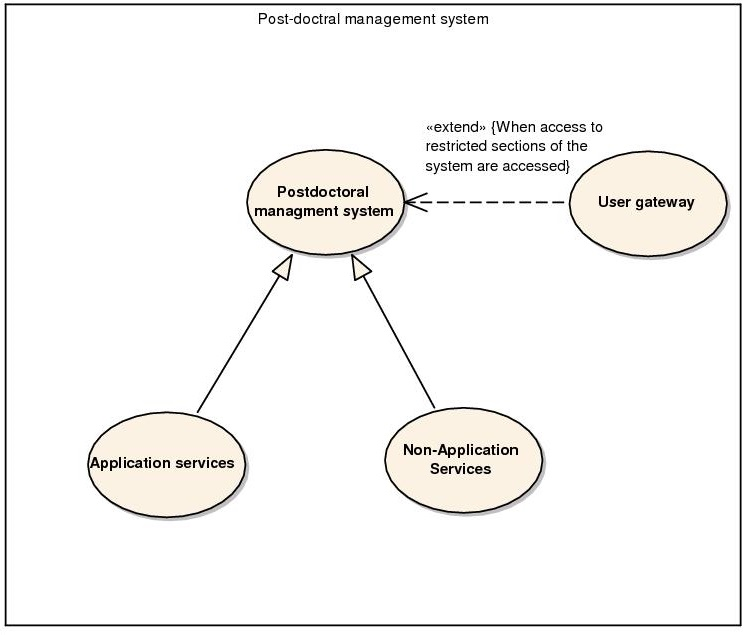
\includegraphics[scale=1]{../Images_Docs/Diagrams/Use case diagrams/Post-doctral fellowship management system1.jpg}}
\caption{Use case diagram of Post-doctoral fellowship management system}
\end{figure}

\begin{figure}[H]
\centering	
\framebox{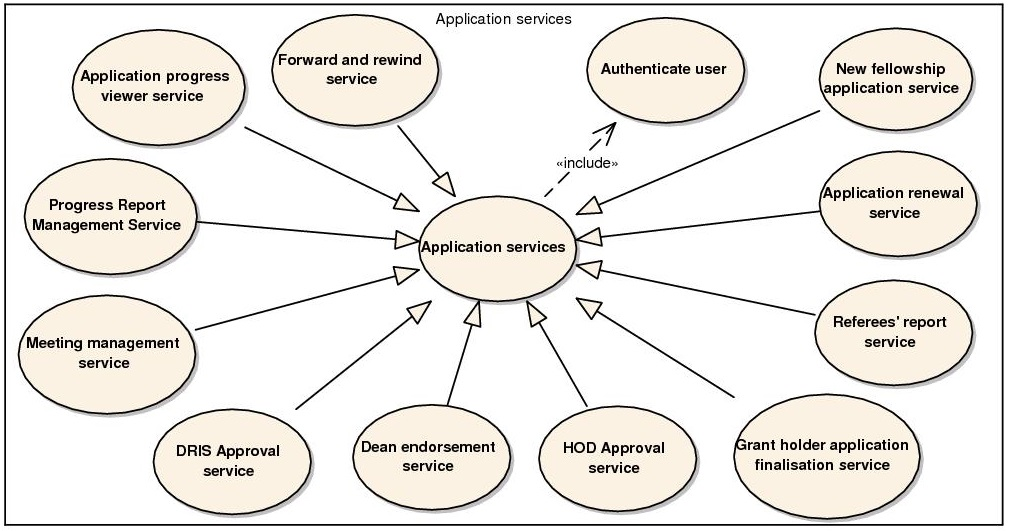
\includegraphics[scale=1]{../Images_Docs/Diagrams/Use case diagrams/Application services1.jpg}}
\caption{Use case diagram of Application service}
\end{figure}

\begin{figure}[H]
\centering	
\framebox{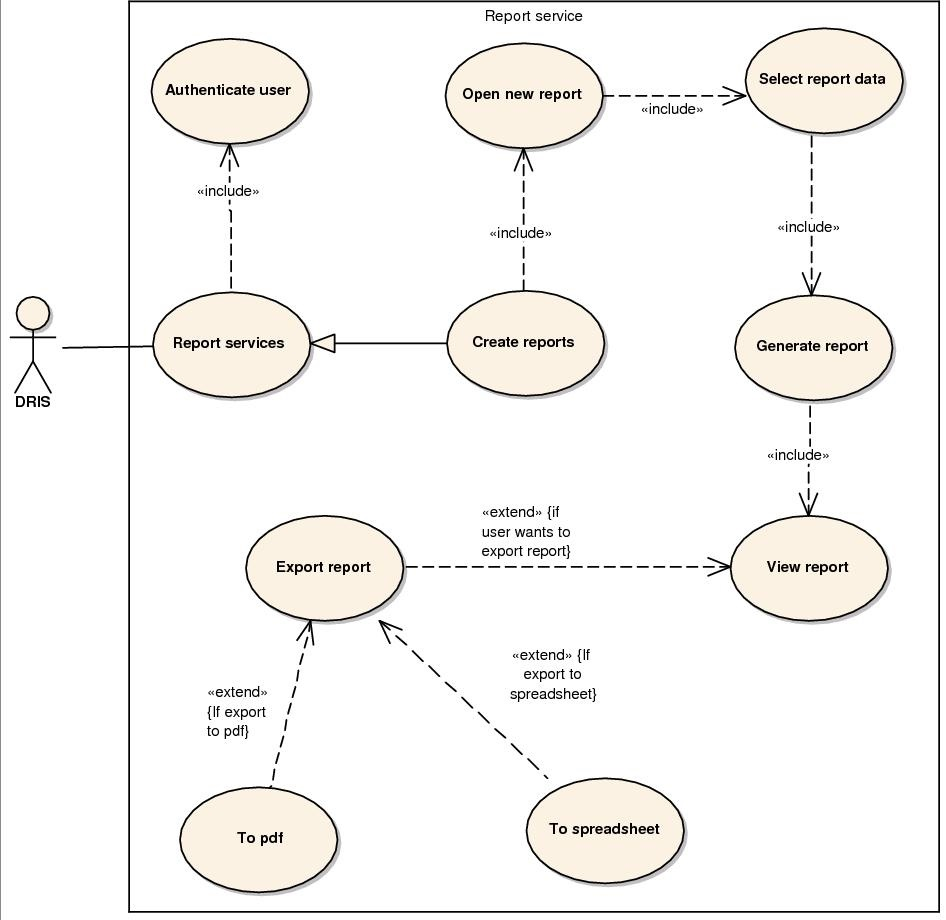
\includegraphics[scale=0.6]{../Images_Docs/Diagrams/Use case diagrams/Report services1.jpg}}
\caption{Use case diagram of Report service}
\end{figure}

\begin{figure}[H]
\centering	
\framebox{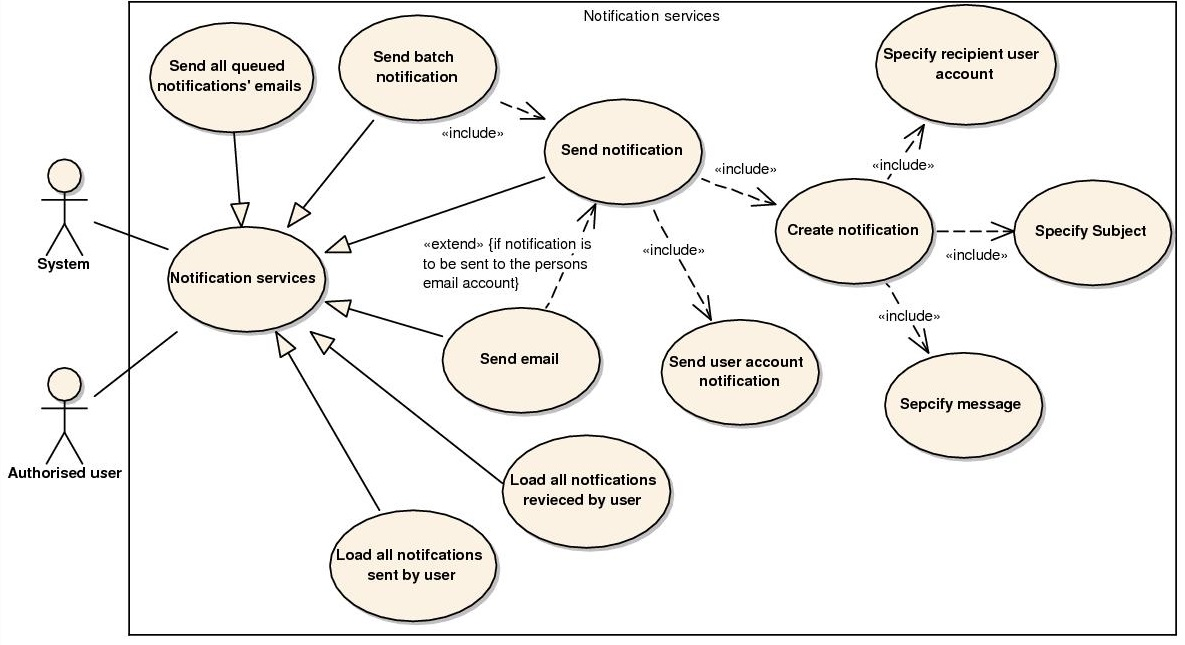
\includegraphics[scale=0.6]{../Images_Docs/Diagrams/Use case diagrams/Notification services1.jpg}}
\caption{Use case diagram of Notification services}
\end{figure}

\begin{figure}[H]
\centering	
\framebox{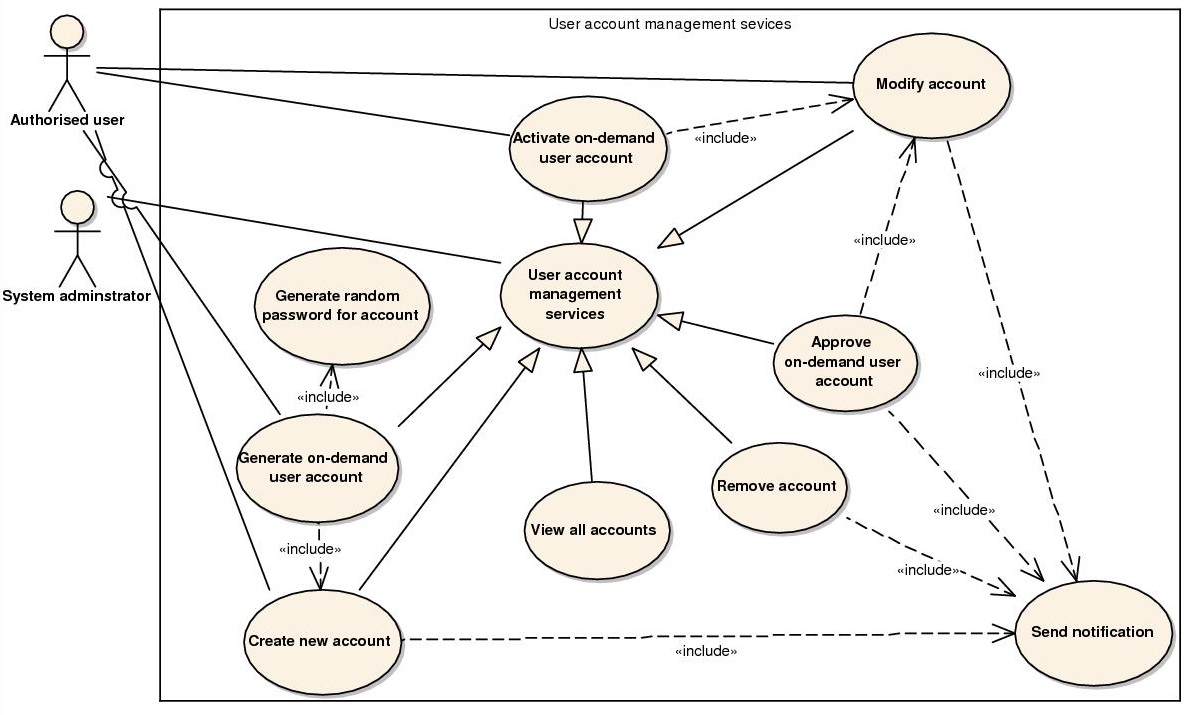
\includegraphics[scale=0.75]{../Images_Docs/Diagrams/Use case diagrams/User account management services1.jpg}}
\caption{Use case diagram of User account management services}
\end{figure}

\begin{figure}[H]
\centering	
\framebox{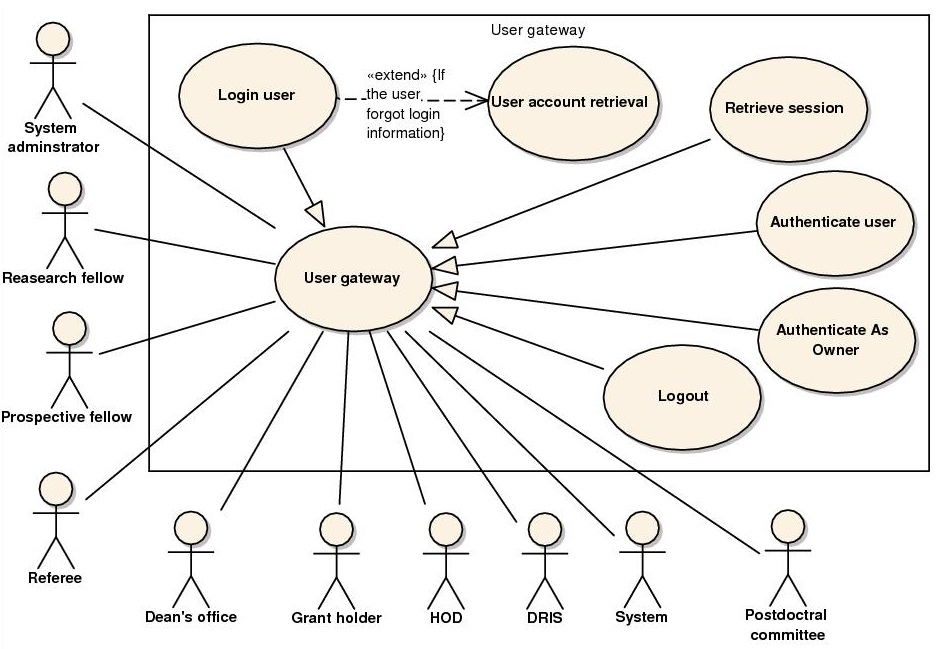
\includegraphics[scale=0.75]{../Images_Docs/Diagrams/Use case diagrams/User gateway1.jpg}}
\caption{Use case diagram of User gateway}
\end{figure}

\begin{figure}[H]
\centering	
\framebox{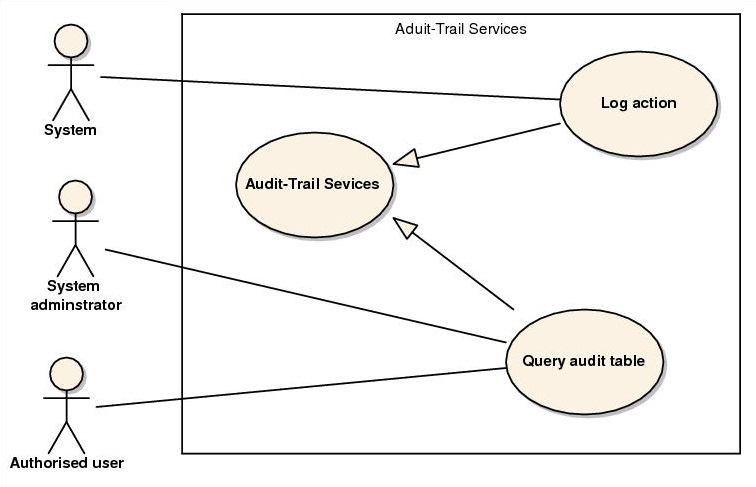
\includegraphics[scale=1]{../Images_Docs/Diagrams/Use case diagrams/Audit-Trail services1.jpg}}
\caption{Use case diagram of Audit-Trail services}
\end{figure}

\begin{figure}[H]
\centering	
\framebox{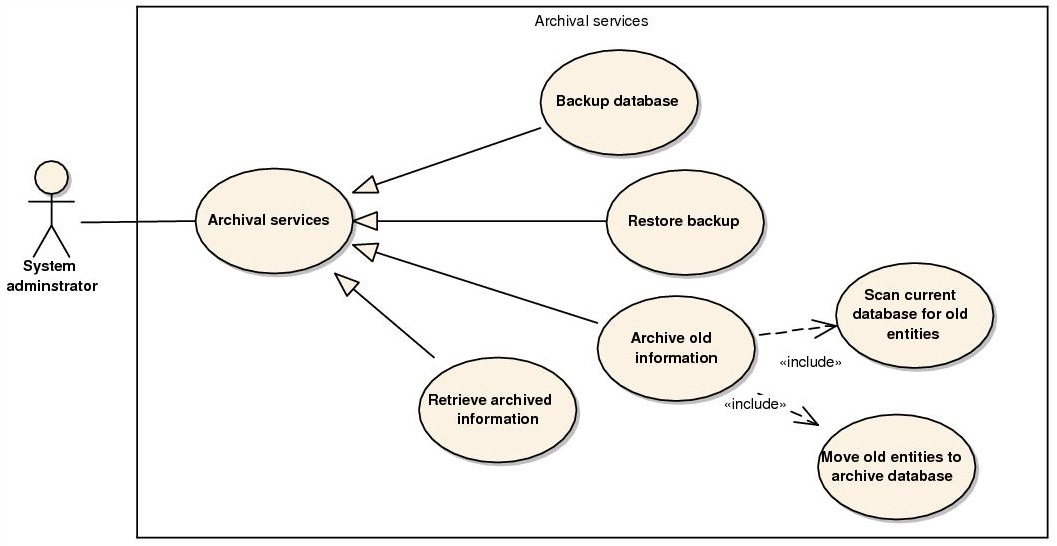
\includegraphics[scale=0.75]{../Images_Docs/Diagrams/Use case diagrams/Archival services1.jpg}}
\caption{Use case diagram of Archival services}
\end{figure}

\begin{figure}[H]
\centering	
\framebox{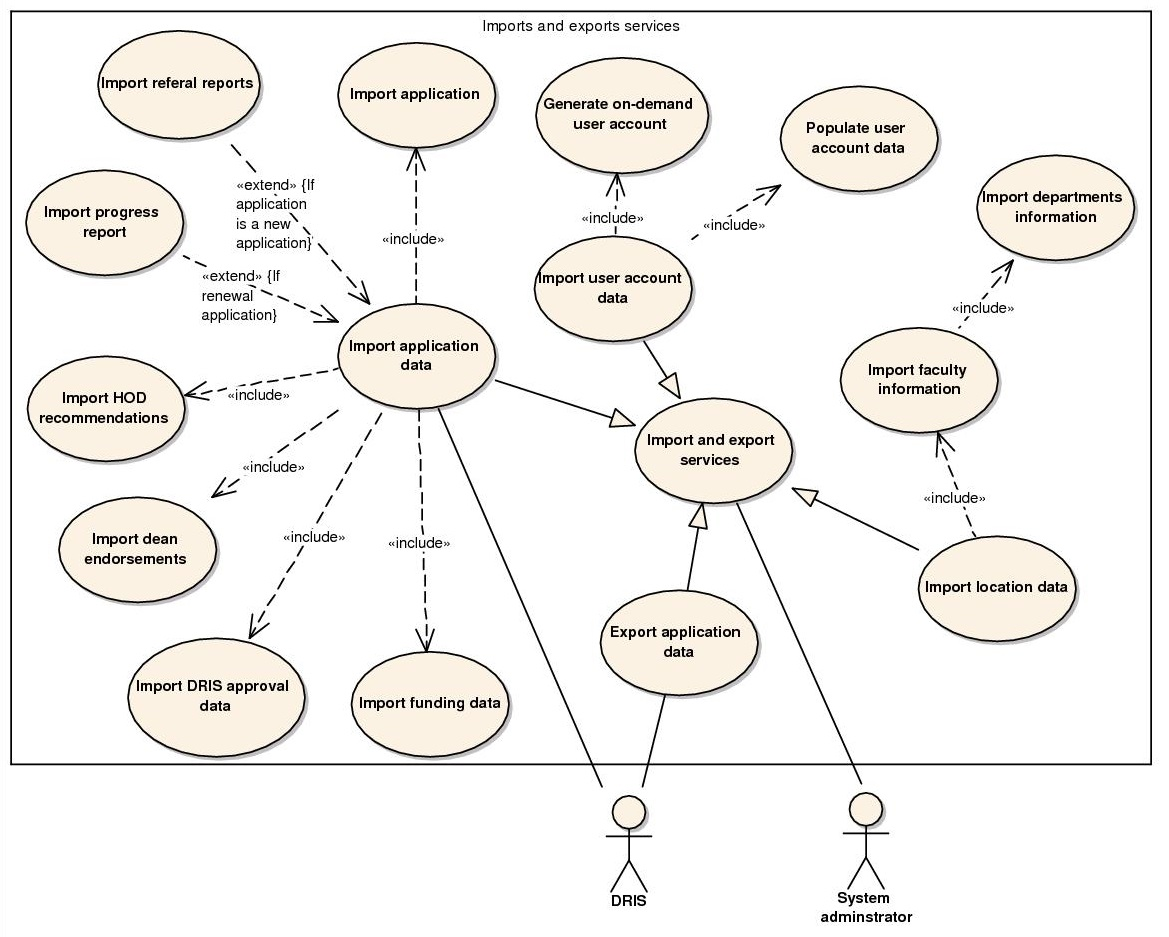
\includegraphics[scale=0.8]{../Images_Docs/Diagrams/Use case diagrams/Imports and exports services1.jpg}}
\caption{Use case diagram of Imports and exports services}
\end{figure}

\begin{figure}[H]
\centering	
\framebox{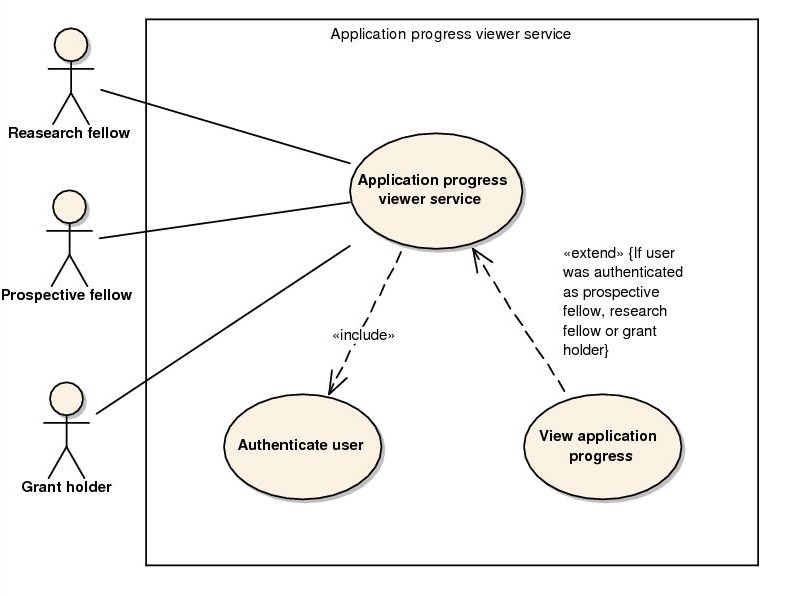
\includegraphics[scale=1]{../Images_Docs/Diagrams/Use case diagrams/Application progress viewer service1.jpg}}
\caption{Use case diagram of Application progress viewer service}
\end{figure}

\begin{figure}[H]
\centering	
\framebox{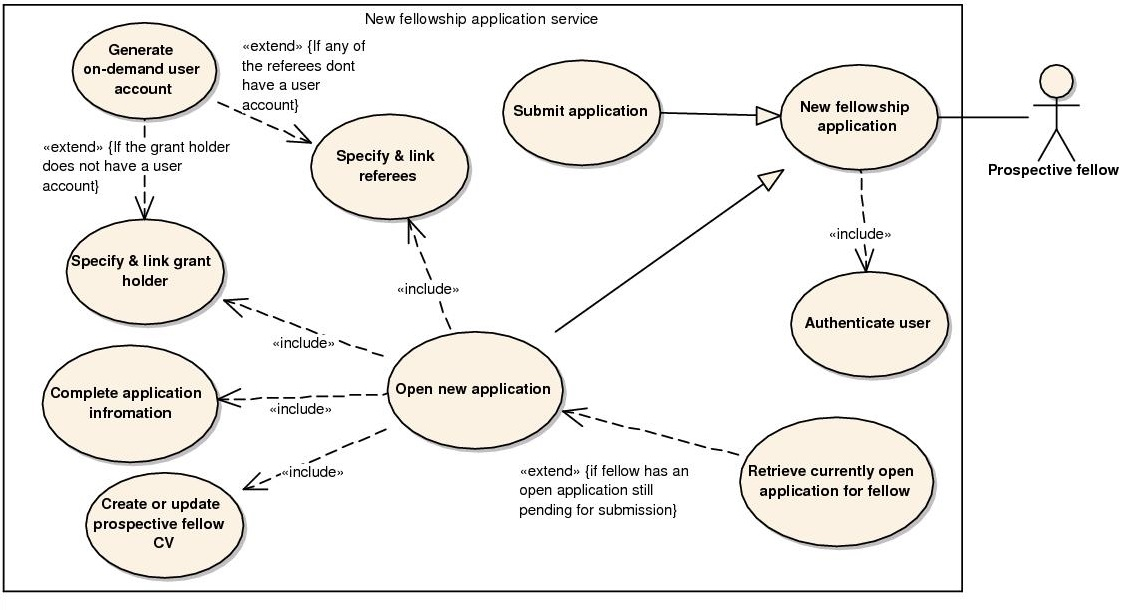
\includegraphics[scale=0.9]{../Images_Docs/Diagrams/Use case diagrams/New fellowship application service1.jpg}}
\caption{Use case diagram of New fellowship application service}
\end{figure}

\begin{figure}[H]
\centering	
\framebox{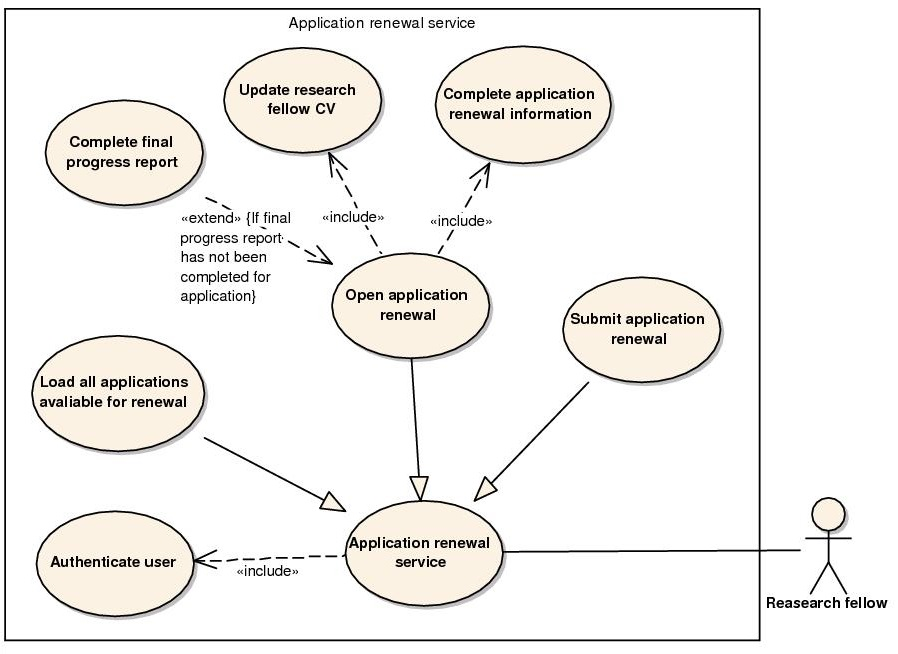
\includegraphics[scale=0.8]{../Images_Docs/Diagrams/Use case diagrams/Application renewal service1.jpg}}
\caption{Use case diagram of Application renewal service}
\end{figure}

\begin{figure}[H]
\centering	
\framebox{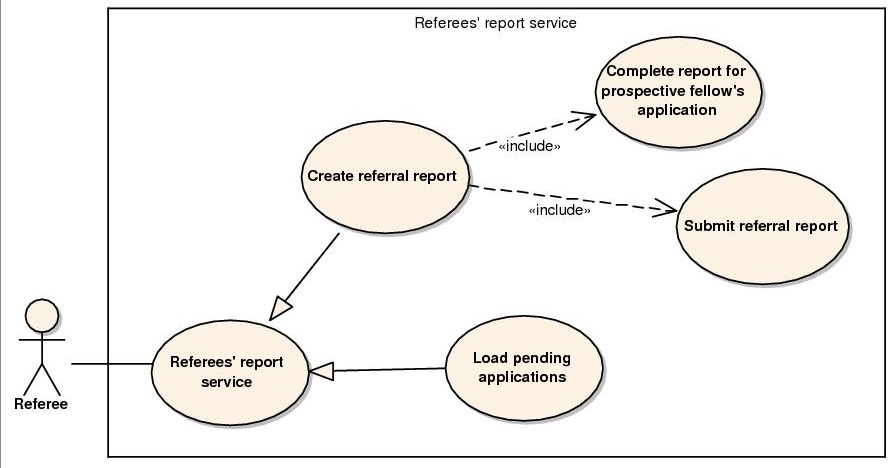
\includegraphics[scale=0.8]{../Images_Docs/Diagrams/Use case diagrams/Referees' report service1.jpg}}
\caption{Use case diagram of Referees' report service}
\end{figure}

\begin{figure}[H]
\centering	
\framebox{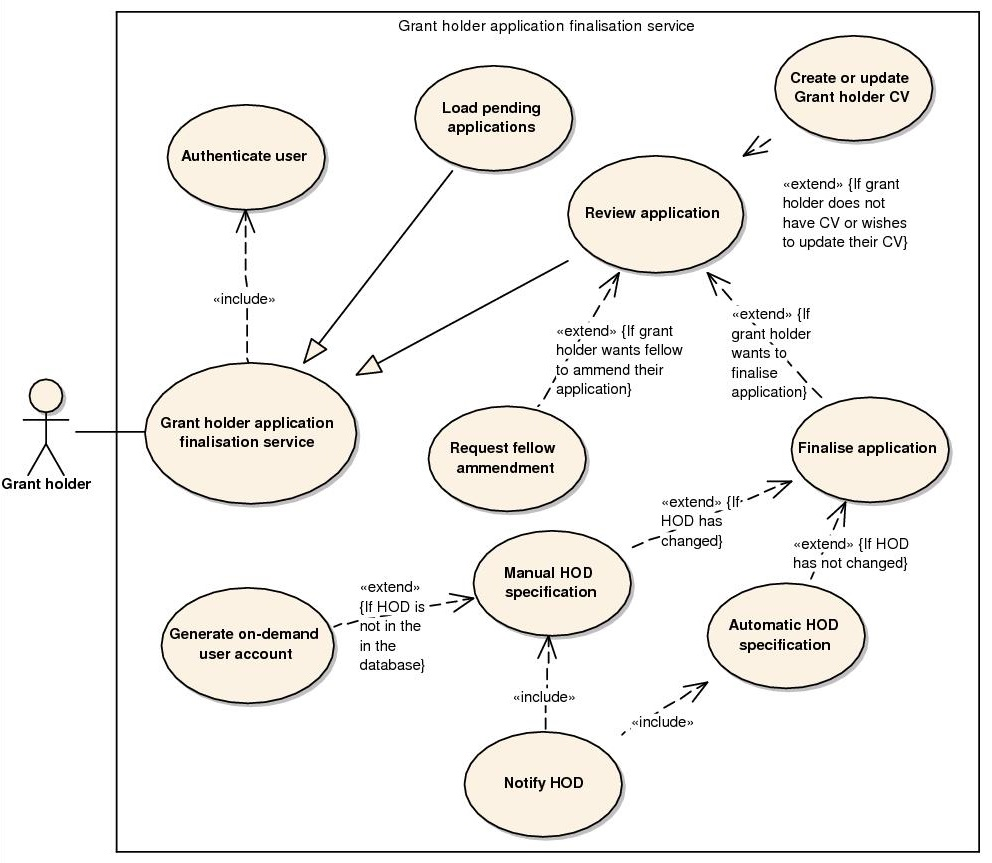
\includegraphics[scale=0.75]{../Images_Docs/Diagrams/Use case diagrams/Grant holder application finalisation service1.jpg}}
\caption{Use case diagram of Grant holder application finalisation service}
\end{figure}

%\begin{figure}[H]
%\centering	
%\framebox{\includegraphics[scale=0.75]{../Images_Docs/Diagrams/Use case diagrams/CV Management service1.jpg}}
%\caption{Use case diagram of CV management service}
%\end{figure}

\begin{figure}[H]
\centering	
\framebox{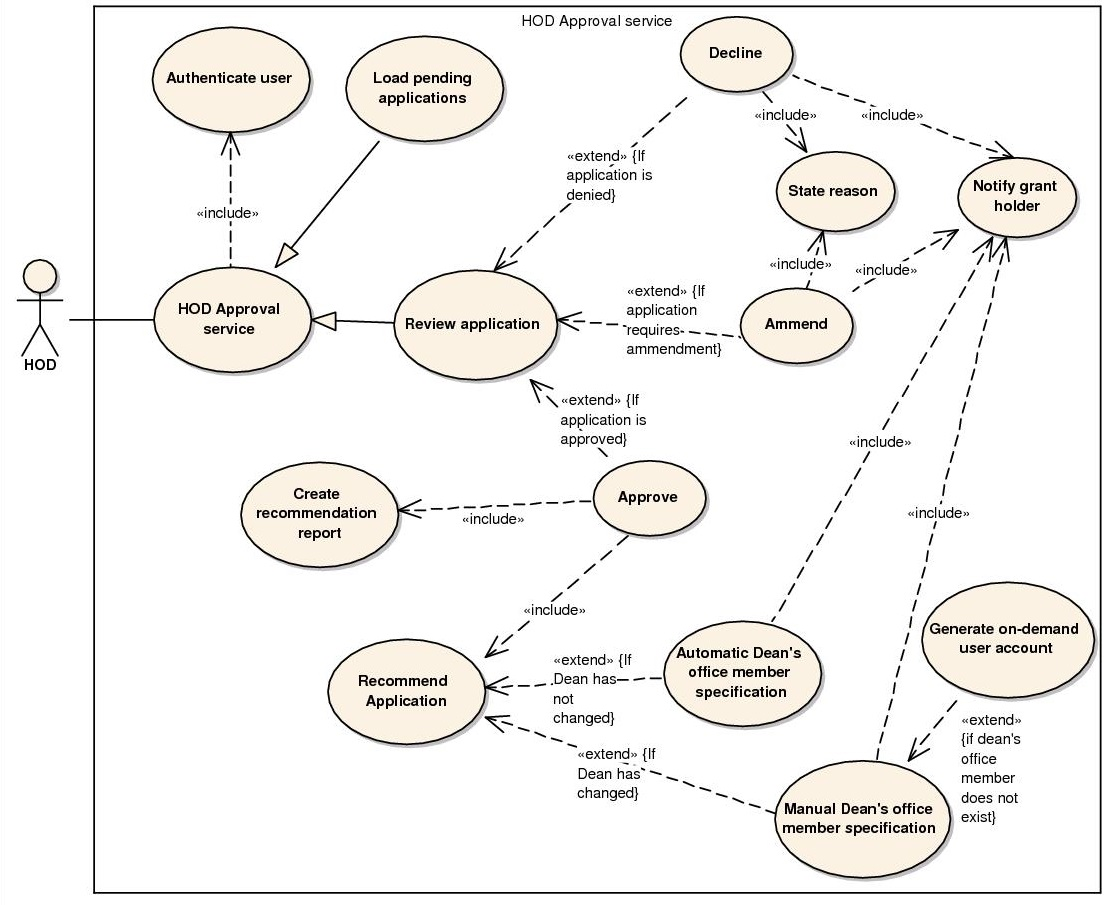
\includegraphics[scale=0.75]{../Images_Docs/Diagrams/Use case diagrams/HOD Approval service1.jpg}}
\caption{Use case diagram of HOD Approval service}
\end{figure}

\begin{figure}[H]
\centering	
\framebox{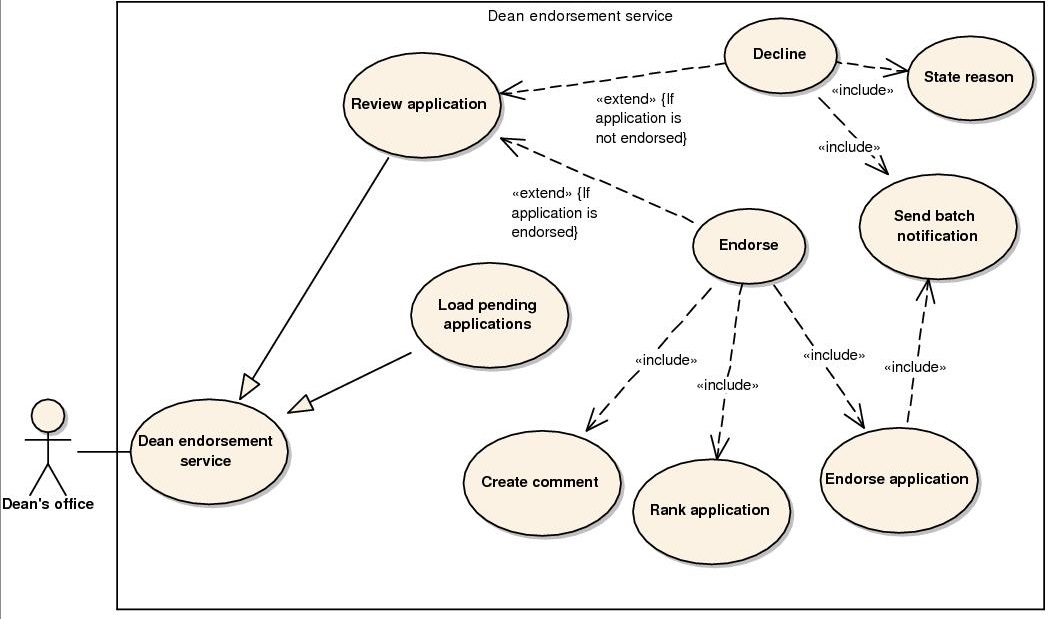
\includegraphics[scale=0.7]{../Images_Docs/Diagrams/Use case diagrams/Dean endorsement service1.jpg}}
\caption{Use case diagram of Dean endorsement service}
\end{figure}

\begin{figure}[H]
\centering	
\framebox{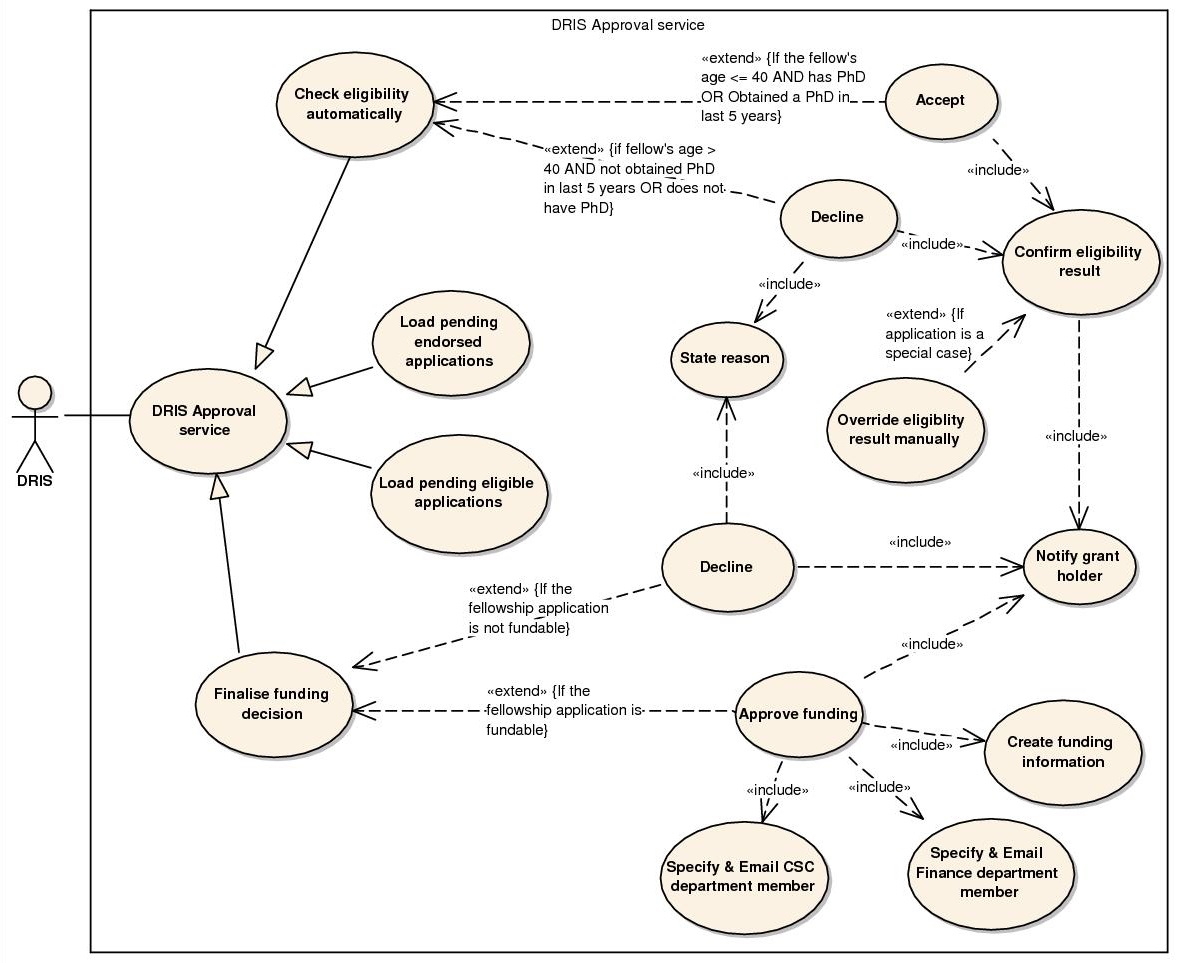
\includegraphics[scale=0.7]{../Images_Docs/Diagrams/Use case diagrams/DRIS approval service1.jpg}}
\caption{Use case diagram of DRIS approval service}
\end{figure}

\begin{figure}[H]
\centering	
\framebox{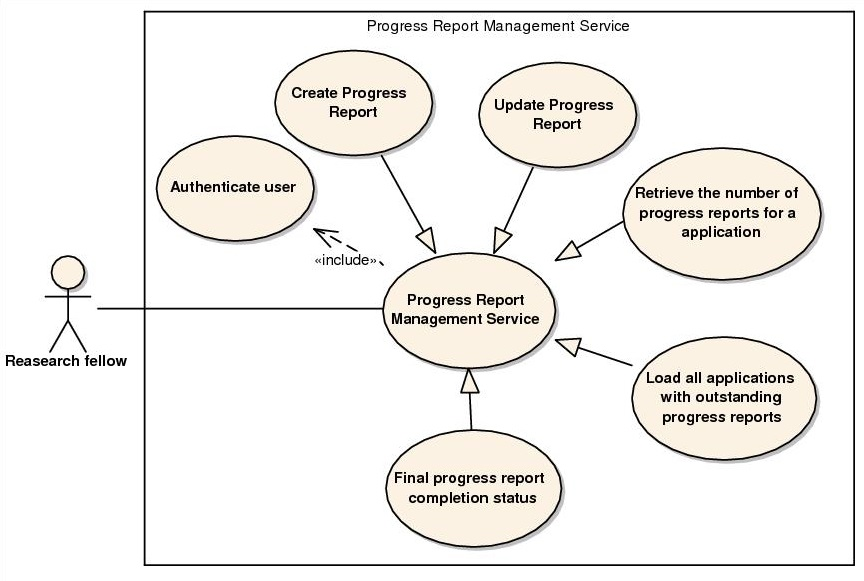
\includegraphics[scale=0.75]{../Images_Docs/Diagrams/Use case diagrams/Progress Report Management Service1.jpg}}
\caption{Use case diagram of Progress Report Management Service}
\end{figure}

\begin{figure}[H]
\centering	
\framebox{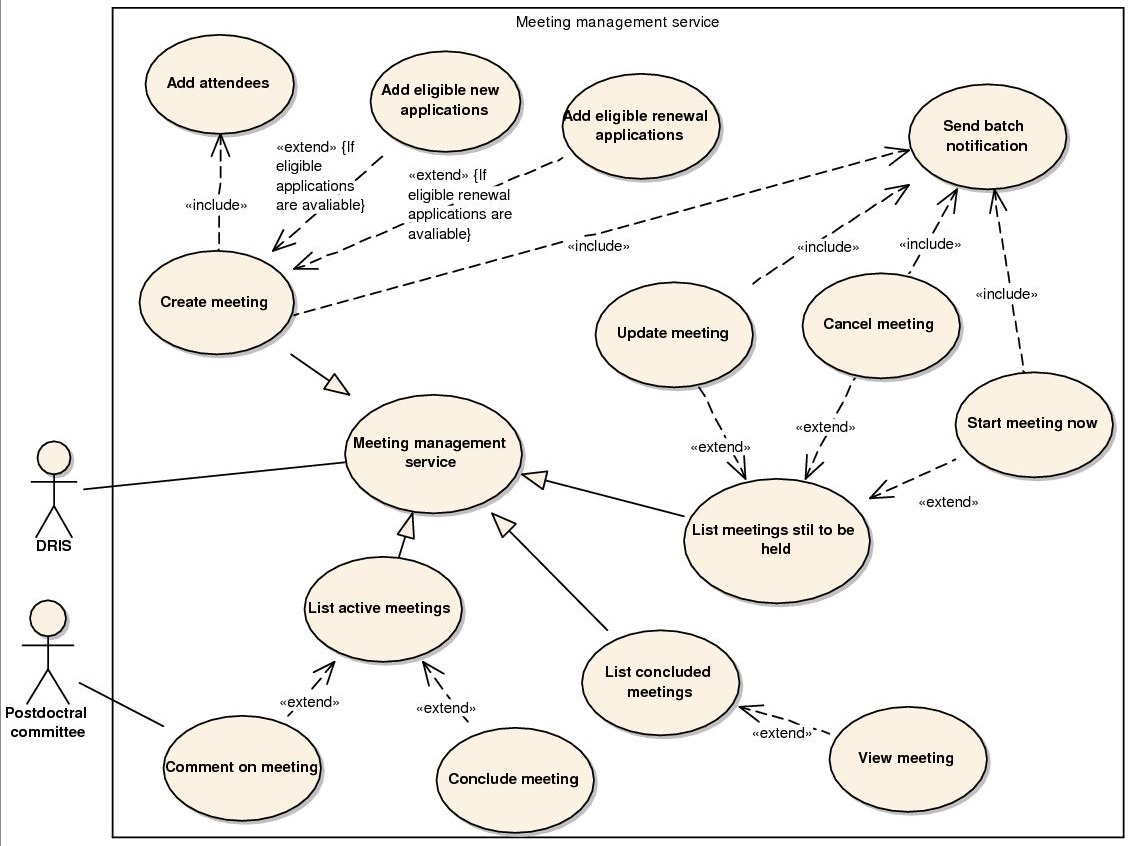
\includegraphics[scale=0.9]{../Images_Docs/Diagrams/Use case diagrams/Meeting management service1.jpg}}
\caption{Use case diagram of Meeting management service}
\end{figure}

\begin{figure}[H]
\centering	
\framebox{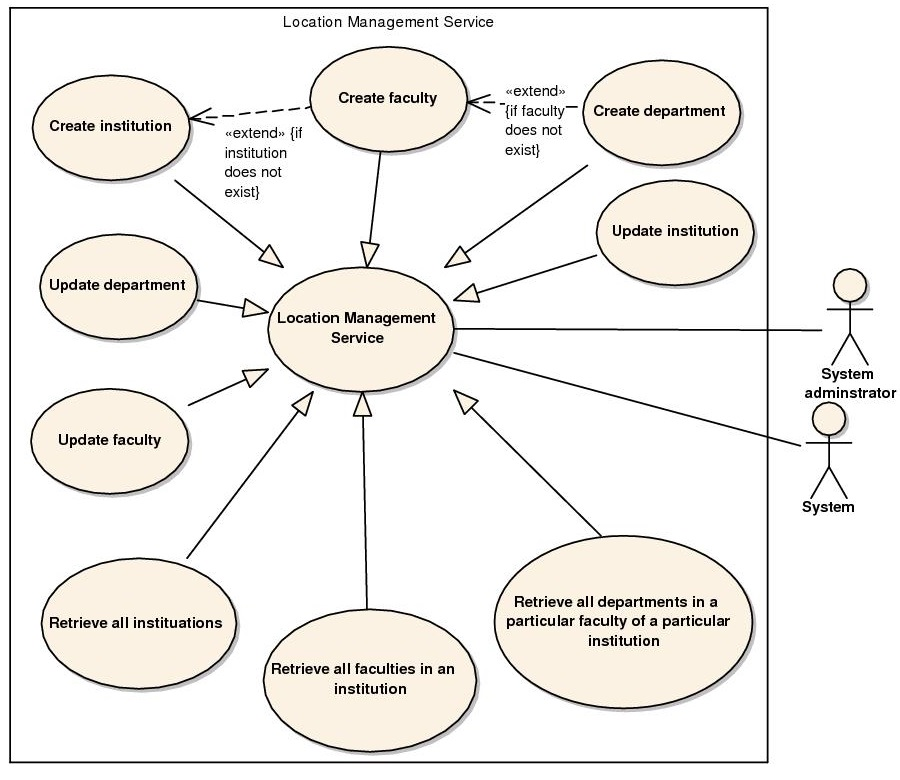
\includegraphics[scale=0.9]{../Images_Docs/Diagrams/Use case diagrams/Location Management Service1.jpg}}
\caption{Use case diagram of Location Management Service}
\end{figure}

\begin{figure}[H]
\centering	
\framebox{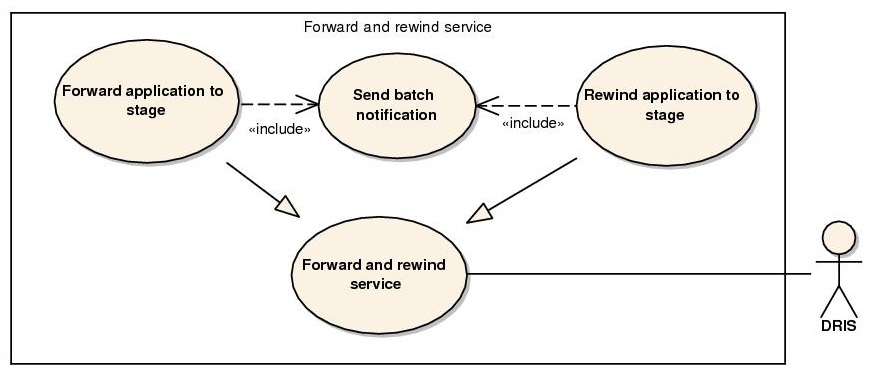
\includegraphics[scale=0.9]{../Images_Docs/Diagrams/Use case diagrams/Forward and Rewind Service1.jpg}}
\caption{Use case diagram of Forward and Rewind Service}
\end{figure}

\newpage
\subsection{Use case prioritization}
\vspace{0.2in}
This section states the ranking in terms of priority of the service use case per use case diagram figure. The priorities are: Critical, Important and Nice to have.\\ 
\begin{itemize}
	\item User gateway: Critical
	\begin{itemize}
		\item Login user: Critical
		\item User account retrieval: Important
		\item Create prospective fellow user account: Critical
		\item Generate on-demand user account: Critical
		\item Activate on-demand user account: Critical
		\item Authenticate user: Critical
	\end{itemize}
	\item Application services: Critical
	\begin{itemize}
		\item New fellowship application service: Critical
		\item Application renewal service: Critical
		\item Referees' report service: Critical
		\item Grant holder application finalisation service: Critical
		\item HOD Approval service: Critical
		\item Dean endorsement service: Critical
		\item DRIS approval service: Critical
		\item Progress report management service: Critical		
		\item Meeting management service: Important
		\item Application progress viewer service: Important		
	\end{itemize}
	\item Notification services: Critical
	\item User account management services: Critical
	\begin{itemize}
		\item Create new account: Critical
		\item Modify account: Critical
		\item Remove account: Important
		\item View all accounts: Important
	\end{itemize}
	\item Audit-Trail services: Critical
	\begin{itemize}
		\item Log action: Critical
		\item Query audit table: Important
	\end{itemize}
	\item CV management service: Critical
	\item Location management service: Critical
	\item Report services: Important
	\item Imports and exports services: Important
	\begin{itemize}
		\item Import user account data: Important
		\item Import application data: Nice to have
		\item Import location data: Important
		\item Export application data: Important
	\end{itemize}	
	\item Archival services: Nice to have
	\begin{itemize}
		\item Retrieve archived information: Nice to have
		\item Archive old information: Nice to have
		\item Backup database: Important
	\end{itemize}
\end{itemize}


\vspace{0.2in}

\subsection{Use case/Services contracts} %Mathys
\vspace{0.2in}

This section states the preconditions and postconditions of the each use case per use case diagram figure. \\

\subsubsection{Preconditions}
These are conditions that must be met by the system or user before they are allowed to use the use case.\\
\begin{itemize}
	\item\textbf{ Application service}
		\begin{itemize}
			\item New fellowship application service: Can only be accessed if new applications are open.
			\item Application renewal service: Can only be accessed if renewals are open and if the user is a research fellow that is still in possession of a fellowship.
			\item Referees' report service:  Can only be accessed if user is a referee.
			\item Grant holder application finalisation service:  Can only be accessed if user is a grant holder.
			\item HOD Approval service:  Can only be accessed if user is a HOD.
			\item Dean endorsement service:  Can only be accessed if user is a member of the dean's office.
			\item DRIS Approval service:  Can only be accessed if user is a member of the DRIS.
			\item Meeting management service:  Can only be accessed if user is a member of the DRIS or post-doctoral committee member.
			\item Application progress viewer service: Can only be accessed if user logged as a prospective fellow, research fellow or grant holder. Also the user needs to have at least one application on the system.	
		\end{itemize}
	
	\item \textbf{Report service}
		\begin{itemize}
			\item Create report: If a user with the associated credentials has been authenticated as a member of the DRIS or with the correct security role.
			\item Open new report: If no report is currently open.
			\item Select report data: If report is open and data is available for report.
			\item Generate report: If data has been selected.
			\item View report: If a report has been generated.
			\item Export report: If user wants to export report and the user is busy viewing the report.
			\item To spreadsheet: If user wants to export report to a spreadsheet.
			\item To pdf: If user wants to export report to a pdf.	
		\end{itemize}
	
	\item \textbf{Notification services}
		\begin{itemize}
			\item Create notification: If requesting user is the system or an authorised user.
			\item Specify recipient user account: If a notification is in its setup stage.				
			\item Specify message: If a notification is in its setup stage.
			\item Send user account notification: If notification is ready to be sent.
			\item Send email: If notification is ready to be sent.	
		\end{itemize}
	
	\item \textbf{User account management services}
		\begin{itemize}
			\item Create new account: If requesting user has the appropriate security role.
			\item Modify account: If requesting user has the appropriate security role or is the owner of the account.				
			\item Remove account: If requesting user has the appropriate security role.	
			\item View all accounts: If requesting user is a system administrator.					
		\end{itemize}
	
	\item \textbf{User gateway}
		\begin{itemize}
			\item Login user: If requesting user is a user of the system.
			\item User account retrieval: If requesting user has forgotten their user credentials.				
			\item Create prospective fellow account: If a new prospective fellow wishes to create an account.	
			\item Activate on-demand user account: If a user has been identified by an applicant and has a security token.
			\item Authenticate user: if user is logged in.						
		\end{itemize}
	
	\item \textbf{Audit-Trail services}
		\begin{itemize}
			\item Log action: If requesting user is the system.
			\item Query audit table: If the user has the correct security role.										
		\end{itemize}
	\item \textbf{Archival services}
		\begin{itemize}
			\item Retrieve archived information: If requesting user is a system administrator or the system.
			\item Archive old information: If requesting user is a system administrator or the system.	
			\item Backup database: If requesting user is a system administrator.					
		\end{itemize}
	\item \textbf{Imports and exports services}
		\begin{itemize}
			\item Import application data: If requesting user is a system administrator or a DRIS member.
			\item Export application data: If requesting user is a system administrator or a DRIS member.	
			\item Import location data: If requesting user is a system administrator.
			\item Import faculty information: If no such faculty is in the database already.
			\item Import departments information: If no such department is in the database and the faculty it relates to is in the database.
			\item Import user account data: If requesting user is a system administrator.
			\item Populate user account data: If the user account exists in th e database and the data is valid.
			\item Import referral reports: If the application is a new application.
			\item Import progress report: If the application is a renewal application.
			\item Import HOD recommendations: If the application has a valid HOD recommendation.
			\item Import dean endorsements: If the application has a valid dean's endorsement.
			\item Import DRIS approval data: If the application has valid DRIS approval data.
			\item Import funding data: If the application has a valid funding data and has been funded.				
		\end{itemize}		
	\item \textbf{Application progress viewer service}
		\begin{itemize}
			\item View application progress: Can only be used if there are any applications made by the user.
		\end{itemize}
		
	\item \textbf{New fellowship application service}
		\begin{itemize}
			\item Generate on-demand user account: If the prospective fellow has identified a referee or grant holder not on the system.
			\item Submit information: If all the application information is complete.
		\end{itemize}
	
	\item \textbf{Application renewal service}
		\begin{itemize}
			\item Open new renewal application: If research fellow has a fellowship that is renewable.
			\item Submit report: If the progress report has been completed.				
			\item Submit renewal application: If all the required information for the renewal has been entered.									
		\end{itemize}
	
	\item \textbf{Referees' report service}
		\begin{itemize}
			\item Load pending applications: If there are any pending applications for the referee and if the user was authenticated as the referee.
			\item Create report: If if a application is selected from the list of pending applications.				
			\item Submit referral report: If the referral report has been completed.									
		\end{itemize}
		
	\item \textbf{Grant holder application finalisation service}
		\begin{itemize}
			\item Load pending applications: If there are any pending applications for the grant holder and if the user was authenticated as the grant holder.
			\item Create Grant holder CV: If grant holder does not have a CV.
			\item Complete application form: If grant holder has selected any application that is still pending.
			\item Submit application: If all the required information has been entered									
		\end{itemize}
			
	\item \textbf{HOD Approval service}
		\begin{itemize}
			\item Load pending applications: If there are any finalised application available for approval and the grant holder of the application falls under department the HOD is in charge of and if user has been authenticated as the HOD.
			\item Application approval: If HOD has selected a application from the application list. 
			\item Create recommendation report: If the application has been approved.				
			\item Submit approved application's information: If the recommendation report has been completed.									
		\end{itemize}
		
	\item \textbf{Dean endorsement service}
		\begin{itemize}
			\item Load pending applications: If there are any approved application available for endorsement and the grant holder of the application falls under faculty of which the Dean's office is in charge of and the user has been authenticated as a member of the dean's office.
			\item Endorse application: If a application is selected from the pending list. 
			\item Rank application: If the application has been endorsed.	
			\item Create comment: If the application has been ranked.			
			\item Submit endorsed application: If the required endorsement information has been completed.									
		\end{itemize}
	
	\item \textbf{DRIS approval service}
		\begin{itemize}
			\item Load pending applications: If the user is authenticated as a member of the DRIS and if there are any endorsed application available for eligibility checking or applications available for finalising their funding decisions.
			\item Check eligibility: If there are any endorsed application available for its eligibility check.
			\item Deny: If the prospective fellow is older than 40 and has not obtained their PhD in the last 5 years or if the prospective fellow does not have a PhD.
			\item Accept: If the prospective fellow is younger than 40 or is 40 and they have a PhD or if they have obtained a PhD in the last 5 years.
			\item Meeting management service: If a meeting is to be created or updated. 
			\item Finalise funding decision: If the meeting regarding the application has been concluded.
			\item Create funding information: The application has been approved for funding.	
			\item Deny: If the application's funding was denied.			
			\item Approve funding: If the application's funding was denied.									
		\end{itemize}
	
	\item \textbf{Meeting management service}
		\begin{itemize}
			\item List options: If user is a authenticated DRIS member.
			\item Create meeting: If any eligible applications are available and the user selects the service from the options list.
			\item Add endorsed applications: If any new applications that are eligible are available.
			\item Add endorsed renewals: If any renewal applications that are eligible are available.
			\item List active meetings: If user is a authenticated post doctoral committee member.
			\item Record minutes of meeting: If the selected meeting has been listed.							
		\end{itemize}
	\end{itemize}

\subsubsection{Postconditions}
These are conditions that must be met by the system and the data after the use case has been used.\\
\begin{itemize}
		
	\item \textbf{Report service}
		\begin{itemize}
			\item Authenticate user: The user has been authenticated as a DRIS member.
			\item Open new report: A new report is active.
			\item Select report data: The data for the active report is selected.
			\item Generate report: The report is available for viewing.
			\item View report: The report is available for export and must be visible.
			\item To pdf: The report has been exported to a PDF file.
			\item To spreadsheet: The report has been exported to a spreadsheet file.	
		\end{itemize}
	
	\item \textbf{Notification services}
		\begin{itemize}
			\item Authenticate user: The user has been authenticated as the system or a user with the appropriate security role.
			\item Send notification: A notification has been stored and sent.
			\item Create notification: A notification has been stored internally.
			\item Specify recipient user account: The notification has a a recipient.				
			\item Specify message: The notification has a message.
			\item Send user account notification: The message is sent to the user.
			\item Send email: The message is sent to the email specified email address.
			\item Send batch notifications: A batch of notifications have been stored and sent.
			\item Load all notifications received by user: All the notifications that were received by the user are available.
			\item Load all notifications sent by user: All the notifications that were sent by the user are available.
		\end{itemize}
	
	\item \textbf{User account management services}
		\begin{itemize}
			\item Create new account: A new user account is added to the system.
			\item Modify account: The specified user account is updated.				
			\item Remove account: The specified user account is disabled and pending removal from the system.
			\item View all accounts: All user accounts have been loaded and are available for viewing.
			\item Generate on-demand user account: A dormant user account has been created on the system with a random password.
			\item Generate random password for account: A random password has been created and associated with account.
			\item Notify owner: A notification has been sent the owner of the account.
			\item Approve on-demand user account: The pending user account has become dormant.
			\item Activate on-demand user account: The dormant user account has become active.						
		\end{itemize}
	
	\item \textbf{User gateway}
		\begin{itemize}
			\item Login user: User is verified and logged in.
			\item User account retrieval: An recovery email is sent to the user account that has been queried for recovery.				
			\item Logout: A user's session has been invalidated and the user is no longer accessing any services of the system.
			\item Retrieve session: The user's session data is available.
			\item Authenticate user as owner: The current user has been authenticated as the owner of the object.
			\item Authenticate user: The user is confirmed to be logged in and has the security role expected by the system.						
		\end{itemize}
		
	\item \textbf{Audit-Trail services}
		\begin{itemize}
			\item Log action: A user action was recorded in the audit table and cannot be changed by user nor by the system.
			\item Query audit table: An valid response to the query was returned.									
		\end{itemize}
	\item \textbf{Archival services}
		\begin{itemize}
			\item Retrieve archived information: The current working database has been repopulated with the selected archive database data.
			\item Archive old information: Any old information in the current working database has moved to the archived database.
			\item Scan current database for old entities: All old entities in the current working database have be identified.
			\item Move old entities to archive database: All old entities are no longer in the current working database but in the archive database.
			\item Backup database: The database has been backed up the specified location.	
			\item Restore backup: The current working database has been repopulated with the backed up data.								
		\end{itemize}
	\item \textbf{Imports and exports services}
		\begin{itemize}
			\item Import application data: All the specified application data is now in the database.
			\item Export application data: All the specified application data has been exported.	
			\item Import location data: All the specified location data is now available in the database. 
			\item Import faculty information: The specified faculty is now in the database.
			\item Import departments information: The specified department is now in the database.
			\item Import user account data: The user account has been created on the system and the user is notified of this.
			\item Populate user account data: The data of the user has been imported into the new user account.
			\item Import referral reports: The associated application's referral reports are in the database.
			\item Import progress report: The associated application's progress report is in the database.
			\item Import HOD recommendations: The associated application's HOD recommendation is in the database.
			\item Import dean endorsements: The associated application's dean endorsement is in the database.
			\item Import DRIS approval data: The associated application's DRIS approval data is in the database.
			\item Import funding data: The associated application's funding data is in the database.				
		\end{itemize}
	\item \textbf{Application progress viewer service}
		\begin{itemize}
			\item Authenticate user: The current user was authenticated as a grant holder or research fellow or a prospective fellow.
			\item View application progress: The application progress of the specified user application is visible.									
		\end{itemize}				
		
	\item \textbf{New fellowship application service}
		\begin{itemize}
			\item Authenticate user: The current user was authenticated as a prospective fellow.
			\item Open new application: A new application has been created and has a status level of open. The prospective fellow is a associated with the application.
			\item Retrieve currently open application for fellow: The current open application of the prospective fellow has been loaded.
			\item Create prospective fellow cv: The prospective fellow's CV has been created and associated with the prospective fellow.
			\item Specify and link grant holder: The grant holder's user account is associated with the application. Grant holder has been notified.
			\item Specify and link referees: The referees' user account is associated with the application. Referees have been notified.
			\item Submit application: The applications status is now submitted.				
		\end{itemize}
	
	\item \textbf{Application renewal service}
		\begin{itemize}
			\item Authenticate user: The current user was authenticated as a research fellow.
			\item Open new renewal application: A new renewal application is open and stored in the system.
			\item Complete final progress report: The final progress report associated with	the renewal has been completed and stored in the system.
			\item Update research fellow CV: The research fellow's CV has been updated.
			\item Complete application renewal information: The application's information is complete and stored. The application associated with the research fellow.		
			\item Submit application renewal: The application status has been set to referred. Grant holder is notified.
			\item Load all applications available for renewal: All the applications of the research fellow which are available for renewal (3 months from expiration) have been loaded.											
		\end{itemize}
	
	\item \textbf{Referees' report service}
		\begin{itemize}
			\item Authenticate user: The current user was authenticated as a referee.
			\item Load pending applications: Any applications that need a referral report from the specified referee must be listed.
			\item Create report for prospective fellow: The report is complete and ready to be submitted.				
			\item Submit referral report: The referral report has been finalised and associated with the application. If it is the last referral report then the application's status is changed to refereed and the Grant Holder of the application is notified.									
		\end{itemize}
	\item \textbf{Grant holder application finalisation service}
		\begin{itemize}
			\item Authenticate user: The current user was authenticated as a grant holder.
			\item Load pending applications: Any applications that need to be finalised from the specified grant holder have been loaded.			
			\item Create or update grant holder cv: The grant holder's CV is stored and associated with the grant holder or is updated.
			\item Review application: The application details have been loaded.
			\item Request fellow amendment: The application's is has reverted to submitted.
			\item Finalise application: The application is now a finalised application. The HOD of the relative department is notified. 
			\item Manual HOD specification: The HOD has been manually specified and notified. If the HOD does not exist in the system a user account has been created for them.
			\item Automatic HOD specification: The HOD has been automatically selected based on location data and has been notified.									
		\end{itemize}
	\item \textbf{CV management service}
			\begin{itemize}
				\item Authenticate User: The user has been authenticated as the System.
				\item Create CV: A CV has been stored on the system and associated with the user.
				\item Update CV: The specified CV has been updated.			
				\item Does CV exist: The status of the CV existence in the system is available.									
			\end{itemize}		
	\item \textbf{HOD Approval service}
		\begin{itemize}
			\item Authenticate user: The current user was authenticated as a HOD.
			\item Load pending applications: Any applications that need to be approved by the specified HOD must have been loaded.
			\item Decline: The specified application's status is changed to declined and a decline report is associated with the application.
			\item Amend: Application's status is changed to refereed. Amend request has been associated with the application.
			\item State reason: The reason for the action is associated with decline report or amend request. 
			\item Notify grant holder: A denied, amend or recommended notification has been sent to the Grant holder of the application appropriately.  
			\item Approve: The application has a recommendation report associated with it and its status has changed to recommended.
			\item Review application: The application details have been loaded.
			\item Create recommendation report: The recommendation report is associated with the application and the Approval is ready to be finalised.				
			\item Recommend application: The application status is changed to recommend. A notification is sent to the grant holder.
			\item Manual Dean's office member specification: The Dean's office member has been manually specified and notified. If the Dean's office member does not exist in the system a user account has been created for them.
			\item Automatic Dean's office member specification: The Dean's office member has been automatically selected based on location data and has been notified.									
		\end{itemize}
		
	\item \textbf{Dean endorsement service}
		\begin{itemize}
			\item Authenticate user: The current user was authenticated as a member of a dean's office.
			\item Load pending applications: Any applications that need to be approved by the specified dean's office have been loaded.
			\item Review application: The application details have been loaded.
			\item Decline: The specified application's status is changed to declined and a decline report is associated with the application.			
			\item State reason: The reason for the action is associated with decline report or amend request. 
			\item Notify grant holder: A denied or endorsed notification has been sent to the Grant holder of the application appropriately.
			\item Endorse: The specified application has been endorsed and has a endorsement report associated with it. The DRIS members are notified.
			\item Rank application: The application has a rank associated with it.	
			\item Create comment: The application has a endorsement comment associated with it.			
			\item Endorse application: The application endorsement is finalised and the application status is now endorsed and the DRIS are notified as well as the grant holder.									
		\end{itemize}
	
	\item \textbf{DRIS approval service}
		\begin{itemize}
			\item Authenticate user: The current user was authenticated as a member of the DRIS.
			\item Load pending endorsed applications: Any applications that need to be checked for eligibility by the DRIS have been loaded.
			\item Load pending eligible applications: Any applications that need to have their final funding decision made by the DRIS have been loaded.			 
			\item Decline: The application eligibility has been automatically declined and is ready to be confirmed. 
			\item Notify grant holder: A decline or eligible or approved funding notification is sent to the Grant holder of the application.
			\item Accept: The application eligibility has been automatically accepted and is ready to be confirmed.			
			\item Decline: The specified application's status is changed to declined and a decline report is associated with the application.			
			\item State reason: The reason for the action is associated with decline report or amend request.			
			\item Check eligibility automatically: The application has been checked for eligibility and been confirmed by the DRIS member.
			\item Confirm eligibility result: The application's status has been changed accordingly. 
			\item Override eligibility result manually: The automated eligibility check's result has been inverted accordingly.
			\item Approve funding: The application status is now changed to a funded.
			\item Create funding information: The application has its funding information associated with it.
			\item Notify grant holder: A notification is sent to the Grant holder of the application that it is successful.
			\item Specify and email CSC department member: A customizable email has been sent to the specified CSC department member.
			\item Specify and email Finance department member: A customizable email has been sent to the specified Finance department member.									
		\end{itemize}
	
	\item \textbf{Progress report management service}
		\begin{itemize}
			\item Authenticate user: The current user was authenticated as a research fellow.
			\item Create progress report: The progress report has stored in the system and is associated with the application.
			\item Update progress report: The specified progress report has been updated.
			\item Retrieve the number of progress reports for a application: The number of progress reports for a application is available.
			\item Load all applications with outstanding progress reports: All applications with outstanding progress reports have been loaded.
			\item Final progress completion status: The completion status of the final progress report for an application is available.							
		\end{itemize}
	
	\item \textbf{Meeting management service}
		\begin{itemize}
			\item Authenticate user: The current user was authenticated as a member of the DRIS or the Post doctoral committee.
			\item List meetings still to be held: All meetings still to be held at the time have been loaded.
			\item List active meetings: All active meetings at the time have been loaded.
			\item List concluded meetings: All concluded meetings at the time have been loaded.
			\item Create meeting: A new meeting is open for modification.
			\item Add endorsed applications: An endorsed new application has been added to the agenda of the meeting.
			\item Add endorsed renewals: An renewal application has been added to the agenda of the meeting.
			\item Add attendee: A attendee have been added to the meeting.
			\item Notify attendees: A notification is sent to all the meeting attendees.			
			\item Comment of meeting: The comment has been associated with meeting.
			\item Start meeting now: The specified meeting has started.
			\item Conclude meeting: The specified meeting has been concluded.
			\item Cancel meeting: The meeting has been cancelled and removed form the system. The attendees have been notified.
			\item Update meeting: The meeting has been updated. The attendees have been notified.
			\item View meeting: The meeting is loaded and being viewed.							
		\end{itemize}
		
	\item \textbf{Forward and Rewind Service}
			\begin{itemize}
				\item Authenticate user: The current user was authenticated as a DRIS office member.
				\item Forward application to stage: The application has been moved to appropriate status.
				\item Rewind application to stage: The application has been moved back to the appropriate stage. All higher stage data has been removed from application.							
			\end{itemize}		

\end{itemize}

\subsubsection{Request and result data structures}
The system will be following a object oriented approach due it being the paradigm of the Java programming language. Therefore the input and output structure will mainly be in the form of objects. Also the objects that will be produced and used inside the system will adhere to the domain objects specification found below.

\vspace{0.2in}
\newpage
\subsection{Process specifications}
\vspace{0.2in}

\begin{figure}[H]
\centering	
\framebox{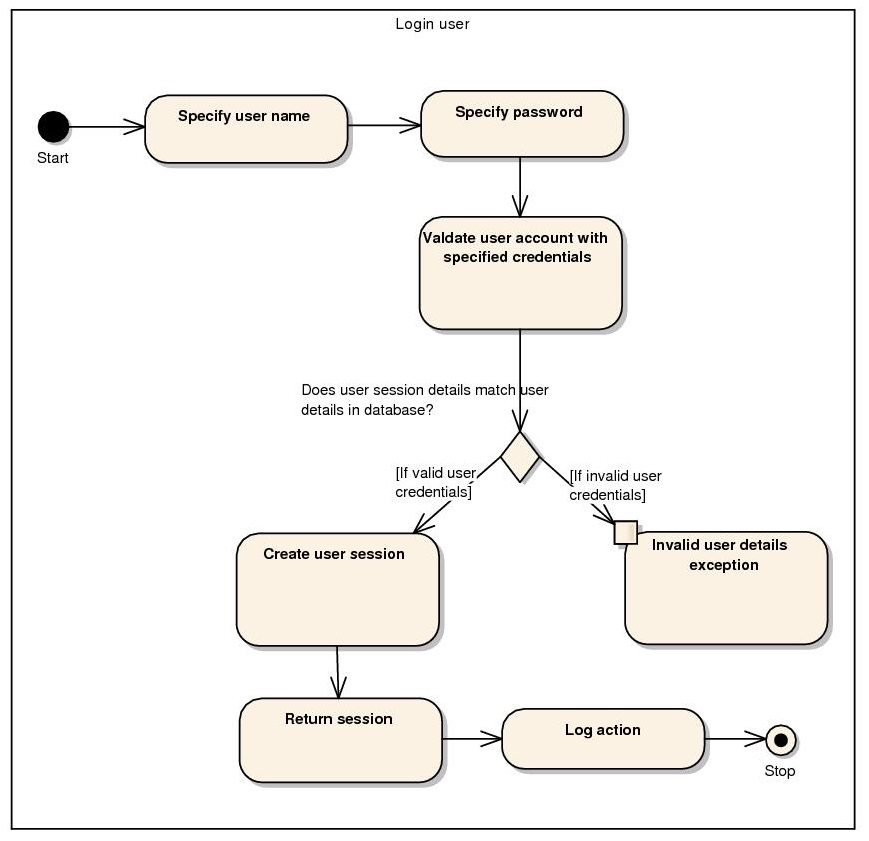
\includegraphics[scale=0.7]{../Images_Docs/Diagrams/Process specs/Login user.jpg}}
\caption{Activity diagram of the Login user use case.}
\end{figure}

\begin{figure}[H]
\centering	
\framebox{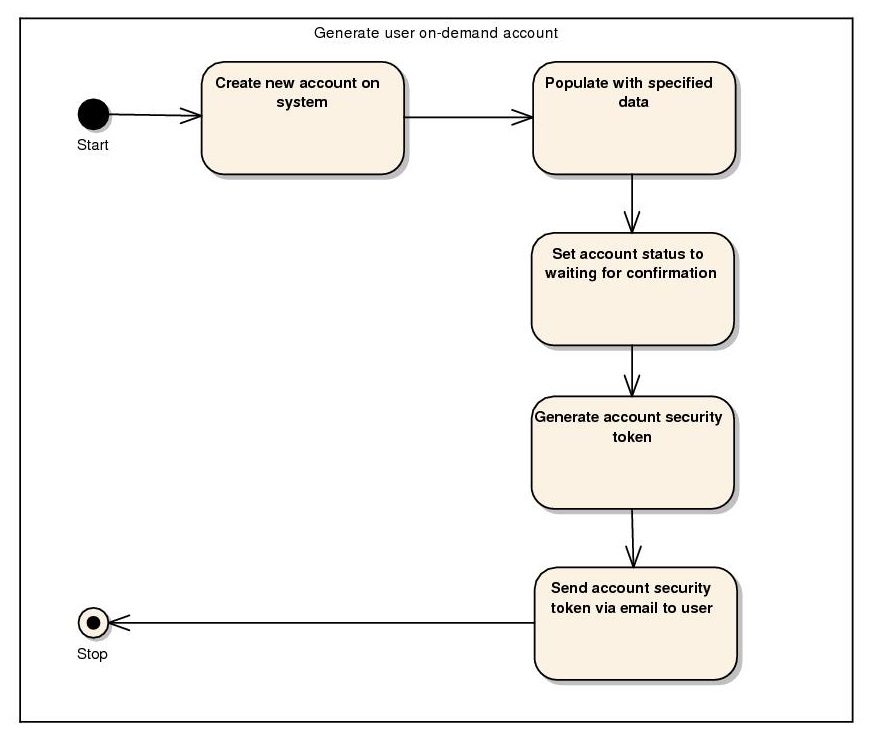
\includegraphics[scale=0.65]{../Images_Docs/Diagrams/Process specs/Generate user on-demand account.jpg}}
\caption{Activity diagram of the Generate user on-demand account use case.}
\end{figure}


\begin{figure}[H]
\centering	
\framebox{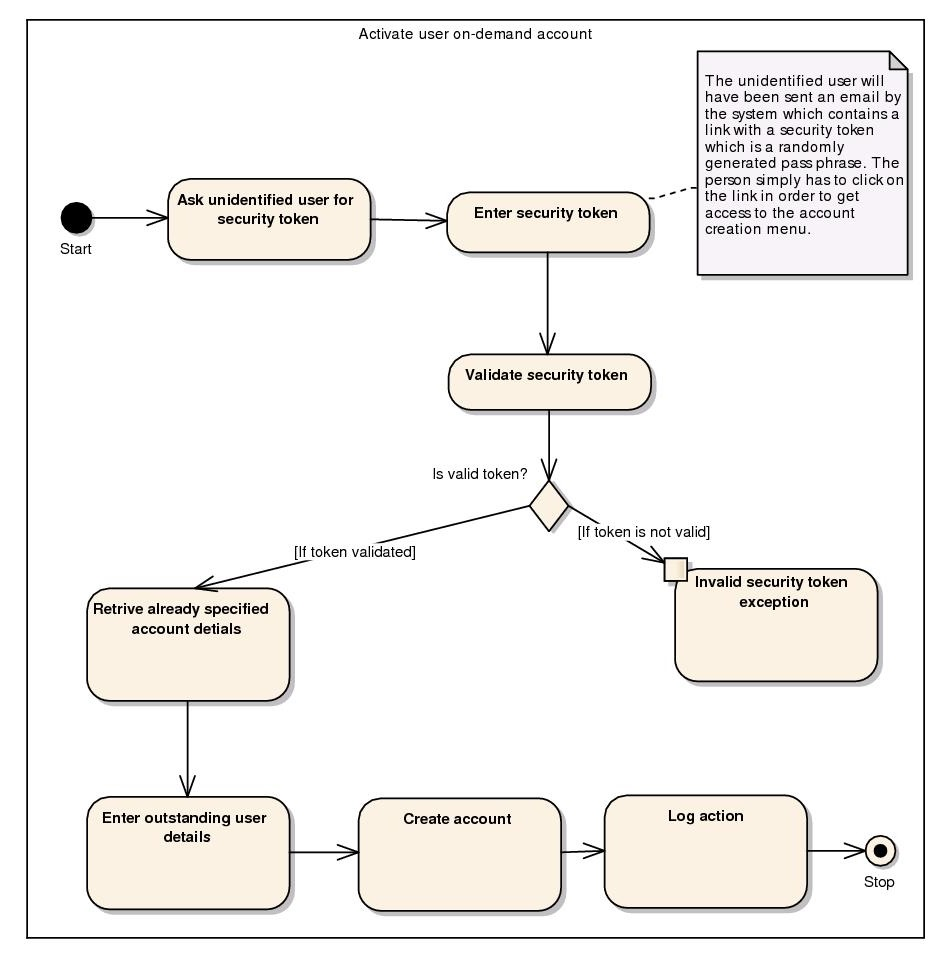
\includegraphics[scale=1]{../Images_Docs/Diagrams/Process specs/Activate user on-demand account.jpg}}
\caption{Activity diagram of the Activate user on-demand account use case.}
\end{figure}

\begin{figure}[H]
\centering	
\framebox{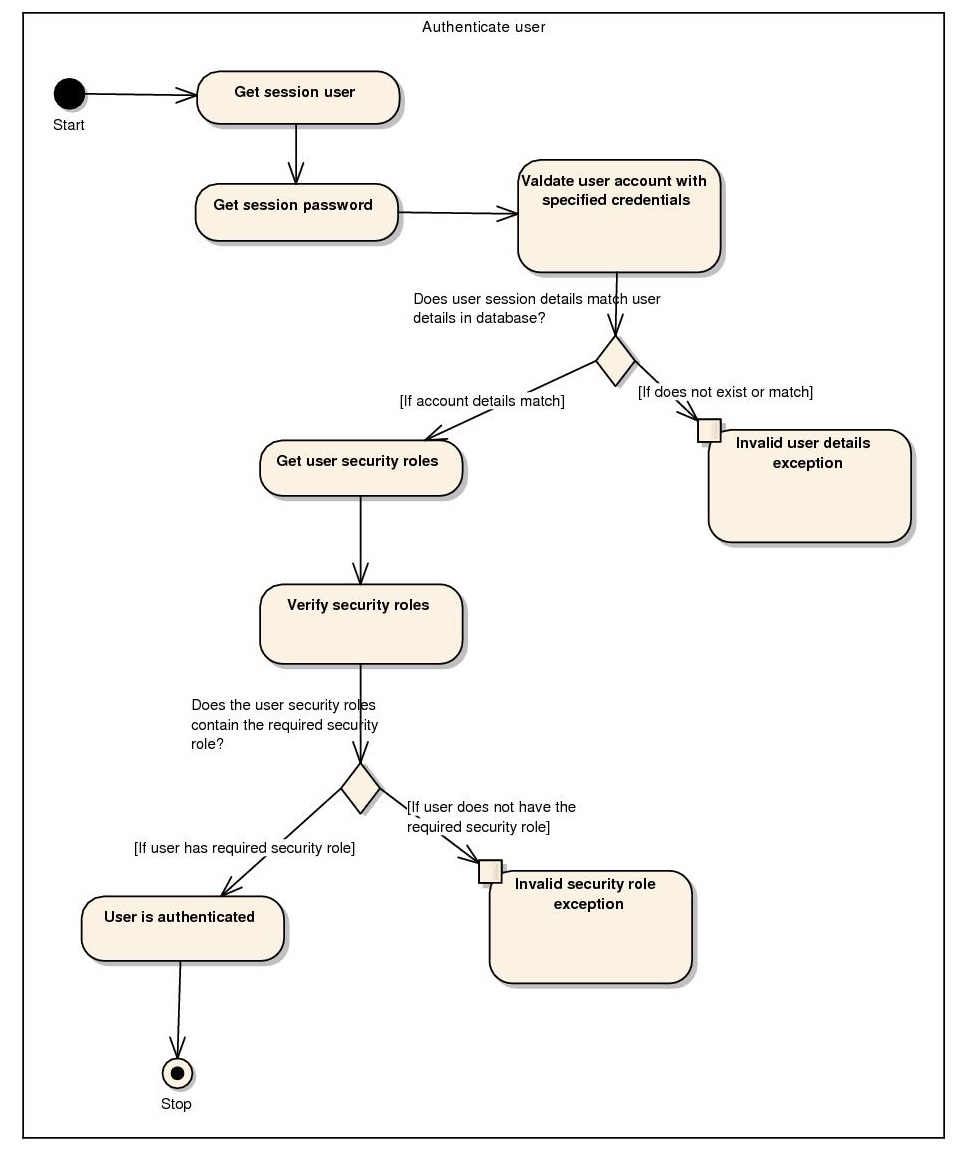
\includegraphics[scale=1]{../Images_Docs/Diagrams/Process specs/Authenticate user.jpg}}
\caption{Activity diagram of the Authenticate user use case.}
\end{figure}

\begin{figure}[H]
\centering	
\framebox{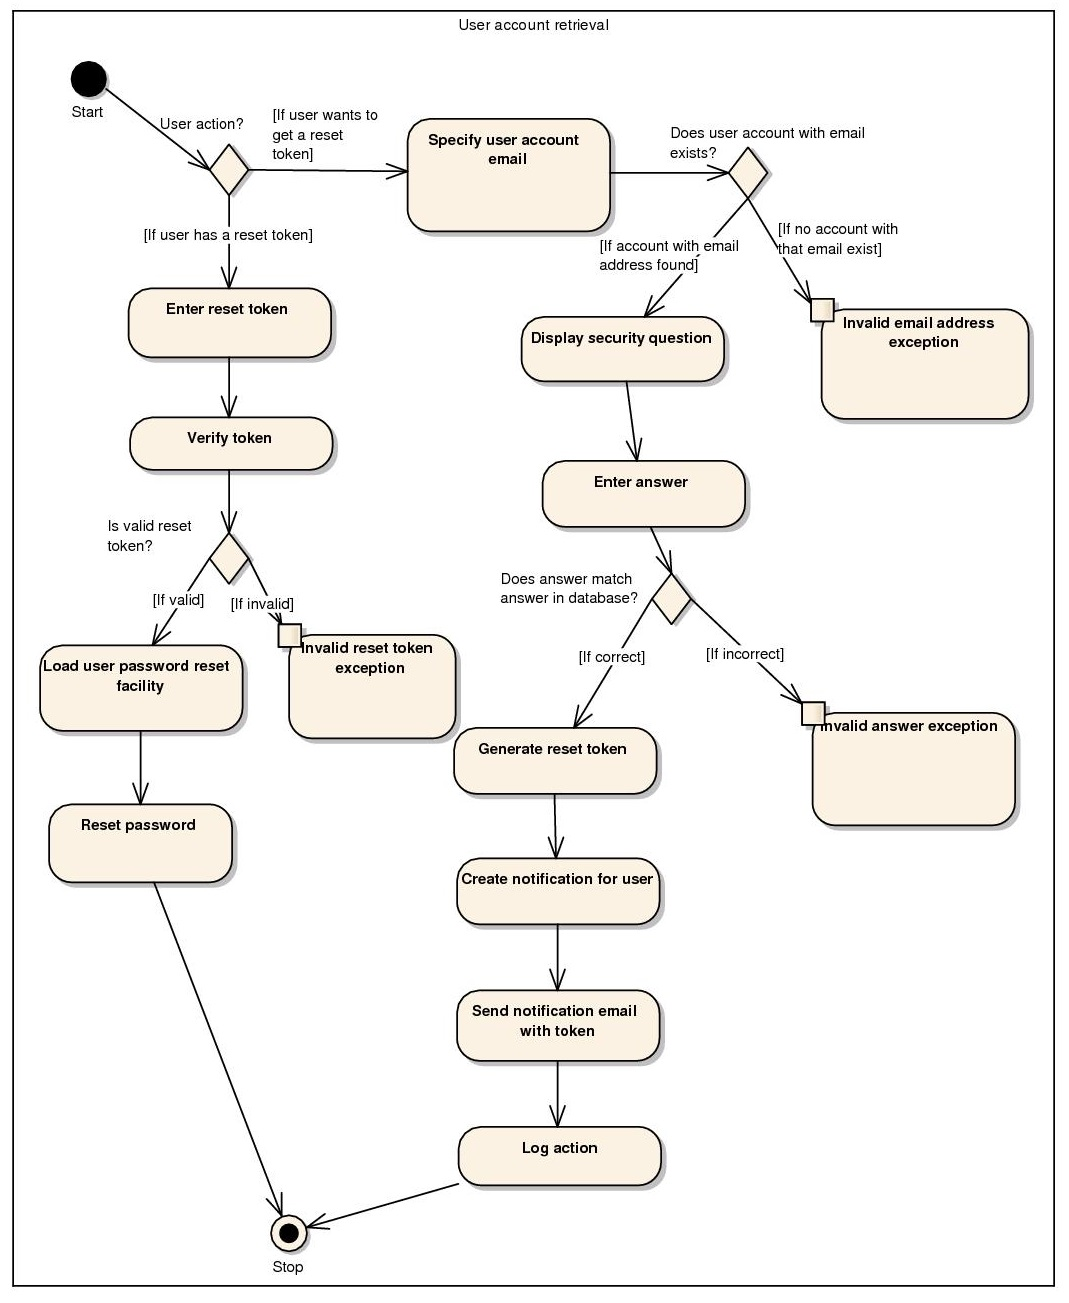
\includegraphics[scale=1]{../Images_Docs/Diagrams/Process specs/User account retrieval.jpg}}
\caption{Activity diagram of the User account retrieval use case.}
\end{figure}

\begin{figure}[H]
\centering	
\framebox{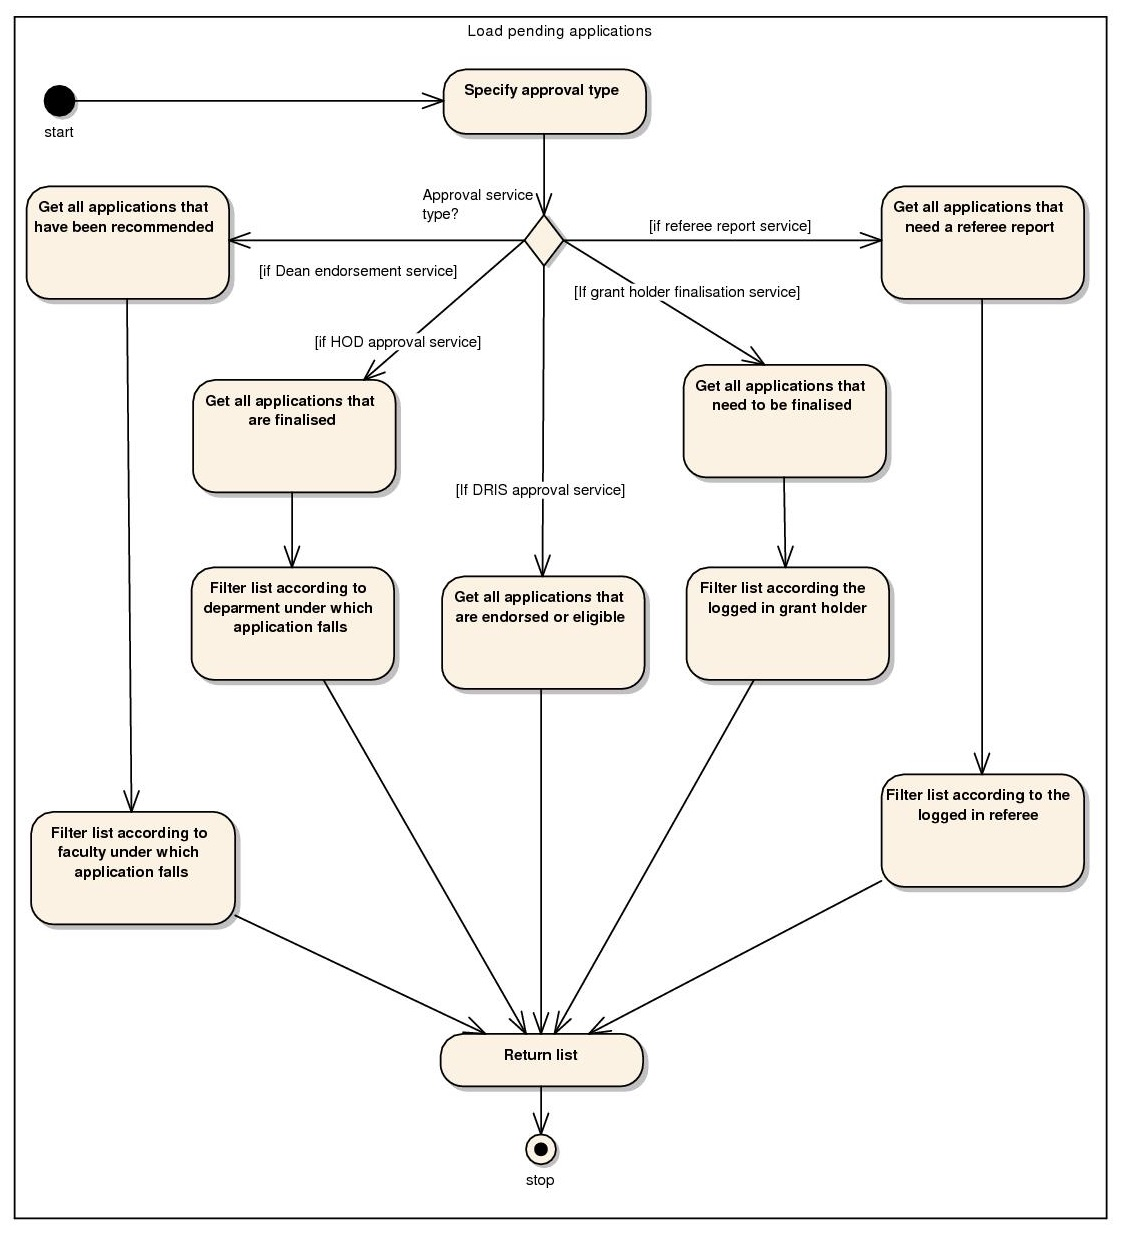
\includegraphics[scale=1]{../Images_Docs/Diagrams/Process specs/Load pending applications.jpg}}
\caption{Activity diagram of the Load pending applications use case.}
\end{figure}

%%%%%%%%%%%%%%%%%%%%%%%%%%%%%%%%%%%%%%%%%%%%%%%%%%%%%%%%%%%%%%%%%%%%%%%%%%%%%%%%%%%%%%%%%%%%%%%%%%%%%%%%%%%%%%%%%%%%%%%%%%%%%%%%%%%%

\begin{figure}[H]
\centering	
\framebox{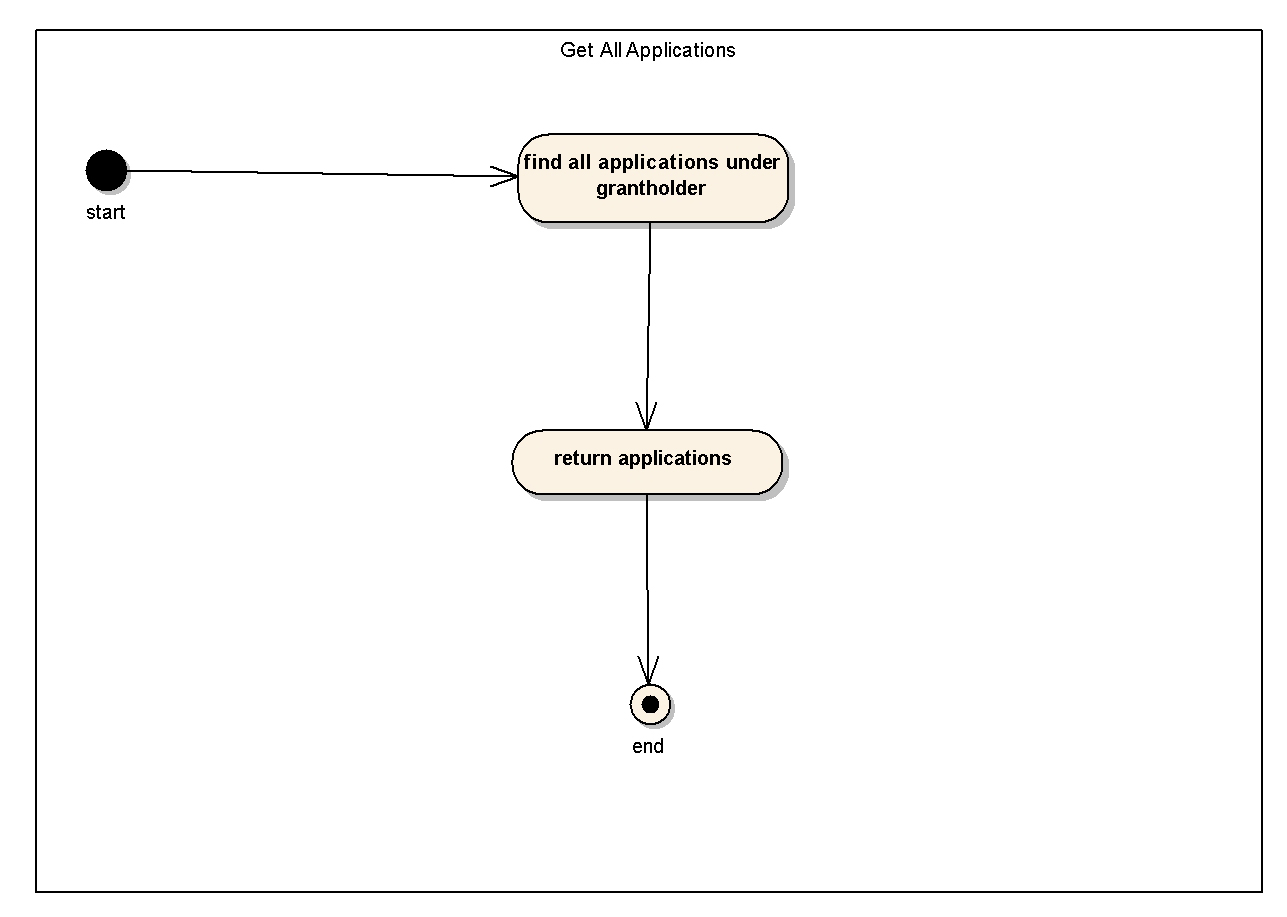
\includegraphics[scale=0.25]{../Images_Docs/Diagrams/Activity Diagrams/ApplicationProgressViewer/Get All Applications.jpg}}
\caption{Activity diagram of the Get All Applications use case.}
\end{figure}

\begin{figure}[H]
\centering	
\framebox{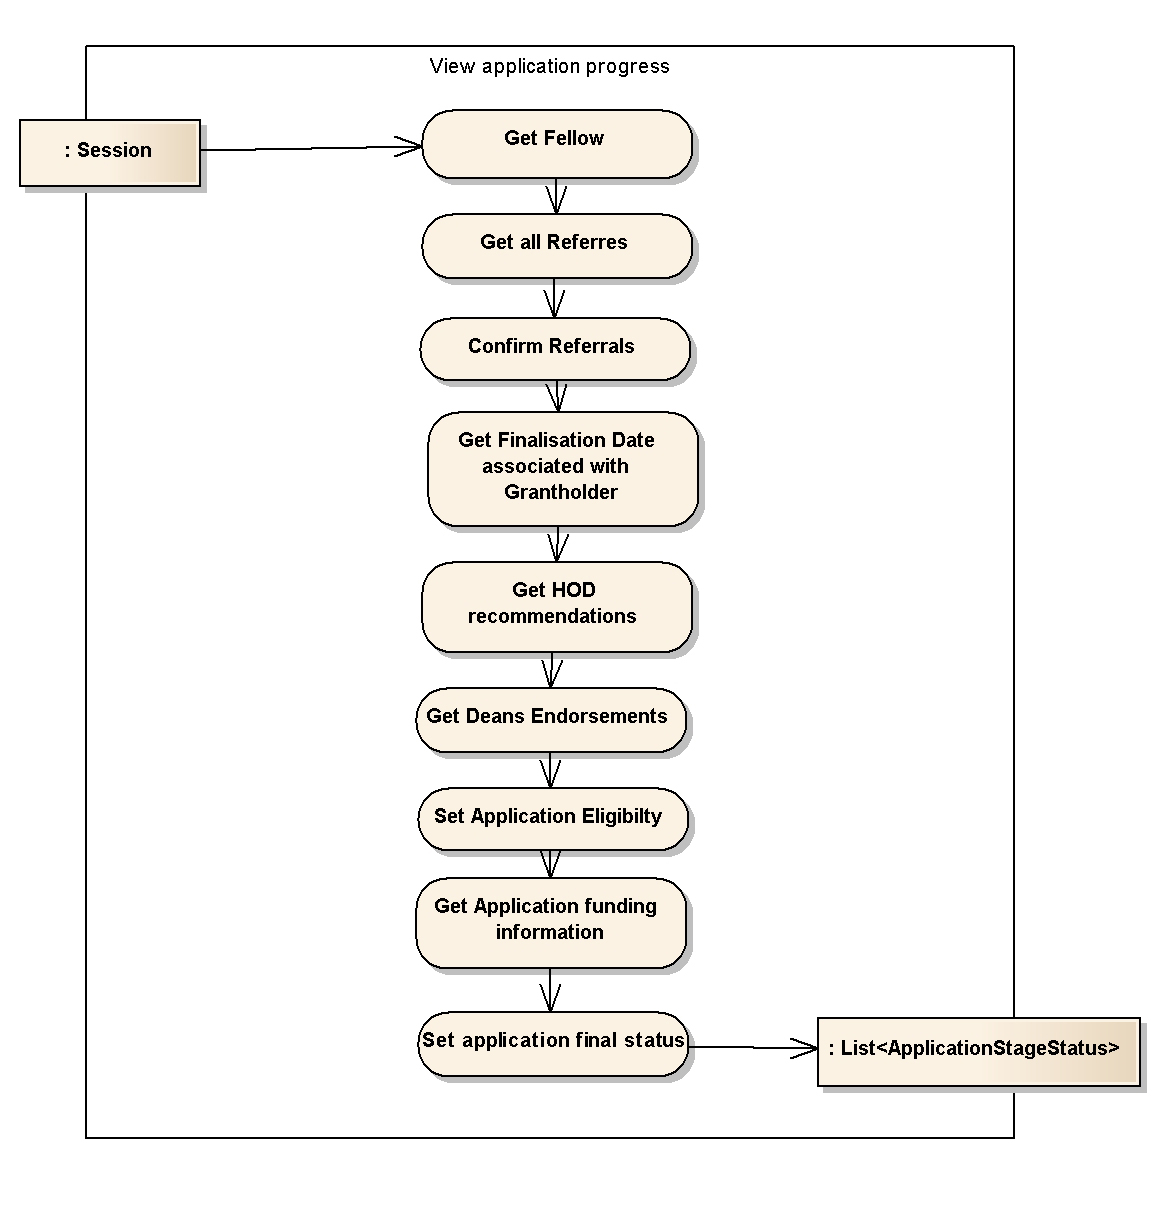
\includegraphics[scale=0.25]{../Images_Docs/Diagrams/Activity Diagrams/ApplicationProgressViewer/View application progress.jpg}}
\caption{Activity diagram of the View application progress use case.}
\end{figure}

%%%%%%%%%%%%%%%%%%%%%%%%%%%%%%%%%%%%%%%%%%%%%%%%%%%%%%%%%%%%%%%%%%%%%%%%%%%%%%%%%%%%%%%%%%%%%%%%%%%%%%%%%%%%%%%%%%%%%%%%%%%%%%%%%%%%

\begin{figure}[H]
\centering	
\framebox{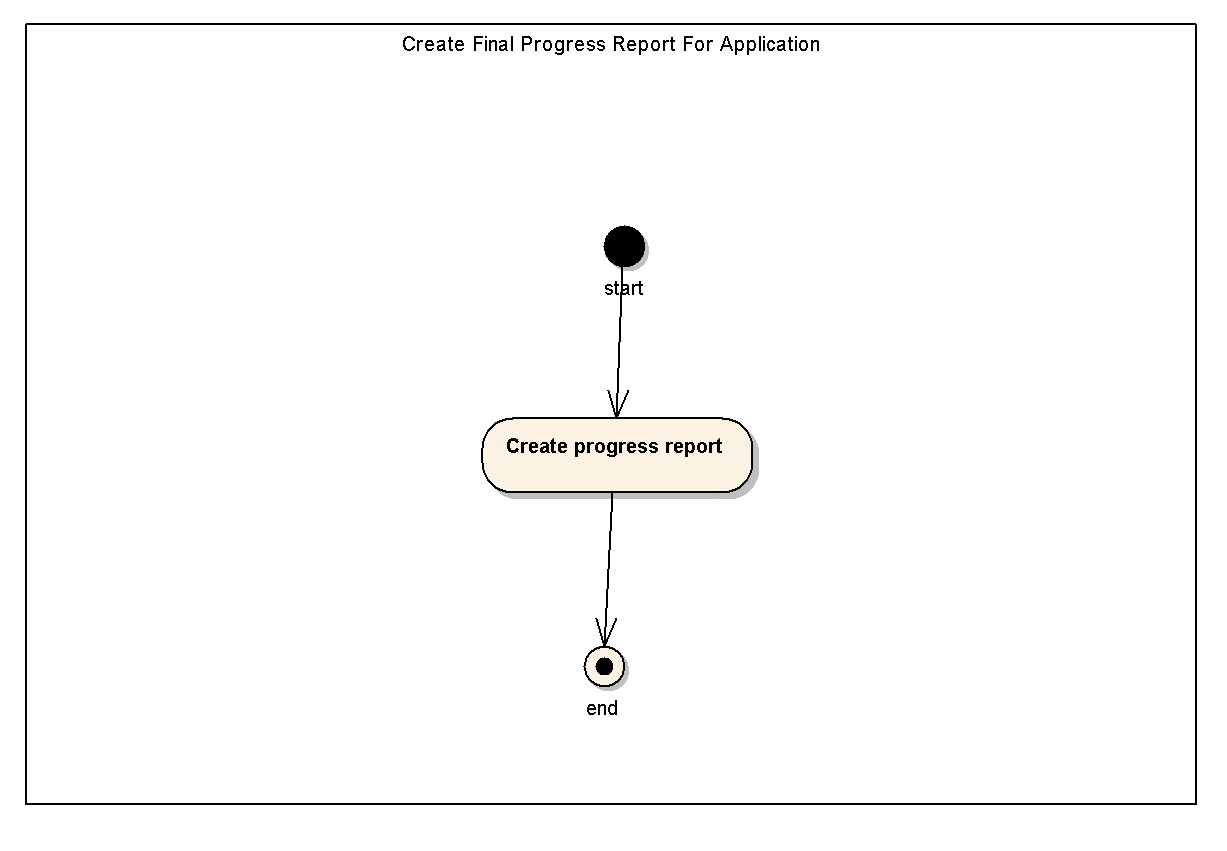
\includegraphics[scale=0.25]{../Images_Docs/Diagrams/Activity Diagrams/ApplicationRenewalService/Create Final Progress Report For Application.jpg}}
\caption{Activity diagram of the Create Final Progress Report For Application use case.}
\end{figure}

\begin{figure}[H]
\centering	
\framebox{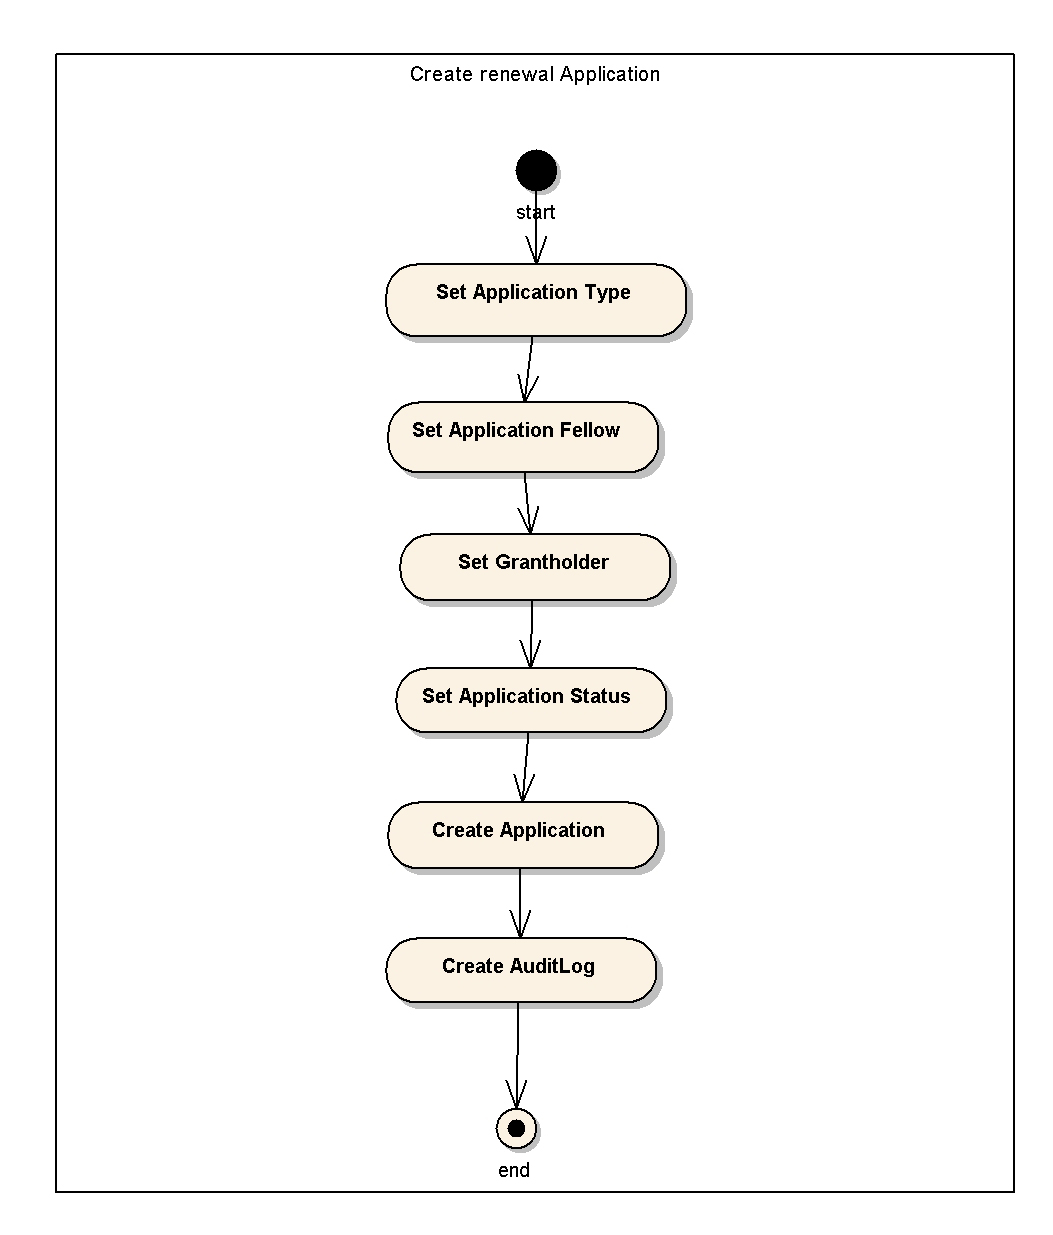
\includegraphics[scale=0.25]{../Images_Docs/Diagrams/Activity Diagrams/ApplicationRenewalService/Create renewal Application.jpg}}
\caption{Activity diagram of the Create renewal Application use case.}
\end{figure}

\begin{figure}[H]
\centering	
\framebox{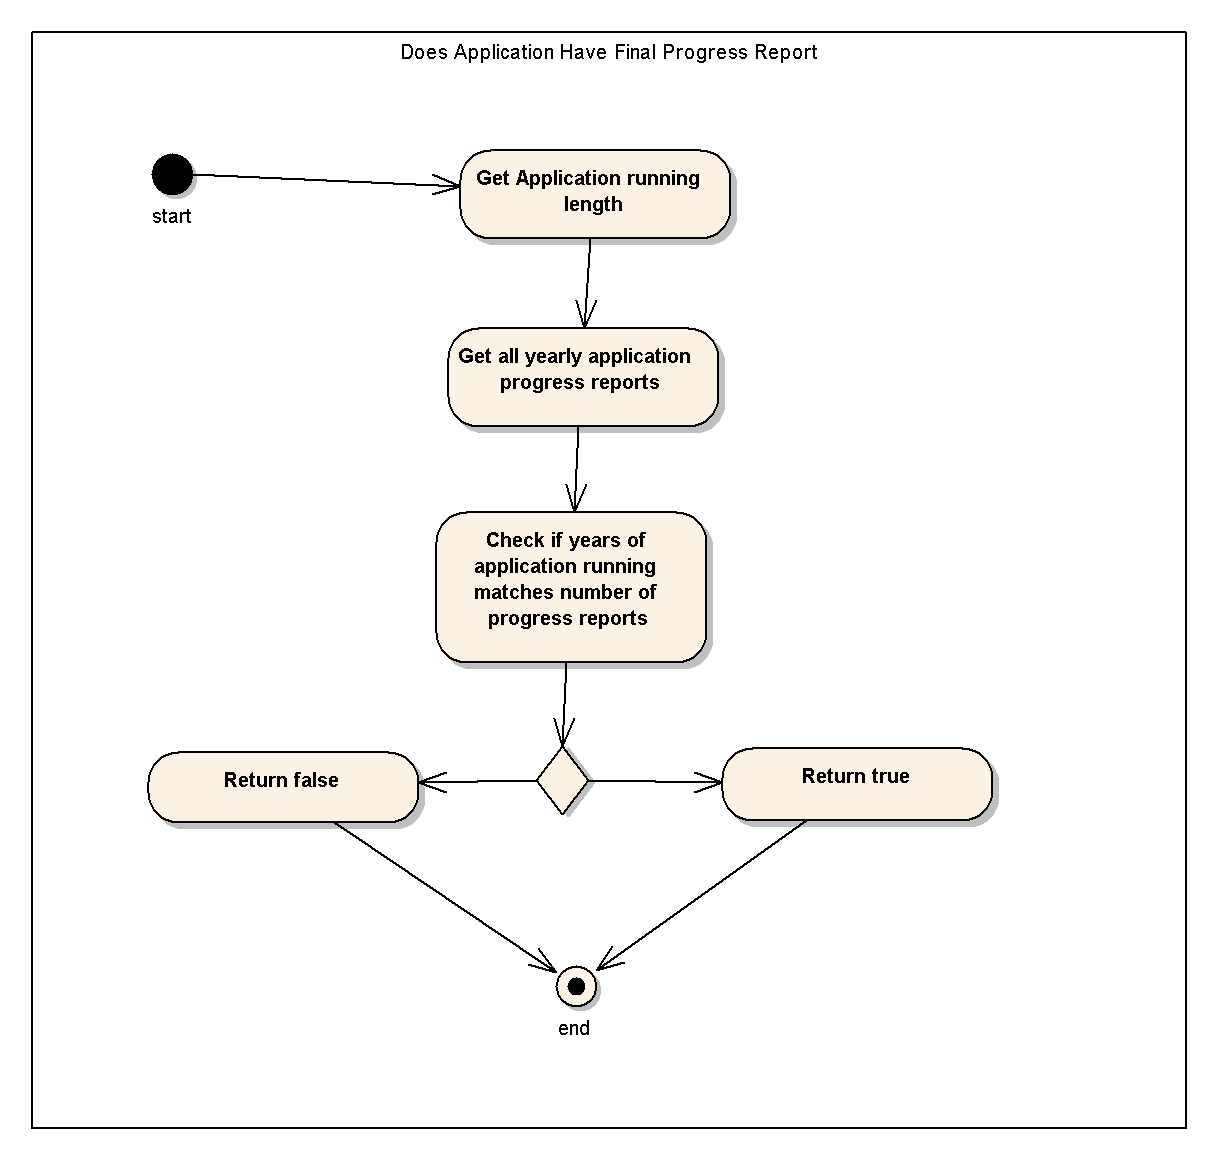
\includegraphics[scale=0.25]{../Images_Docs/Diagrams/Activity Diagrams/ApplicationRenewalService/Does Application Have Final Progress Report.jpg}}
\caption{Activity diagram of the Does Application Have Final Progress Report use case.}
\end{figure}

\begin{figure}[H]
\centering	
\framebox{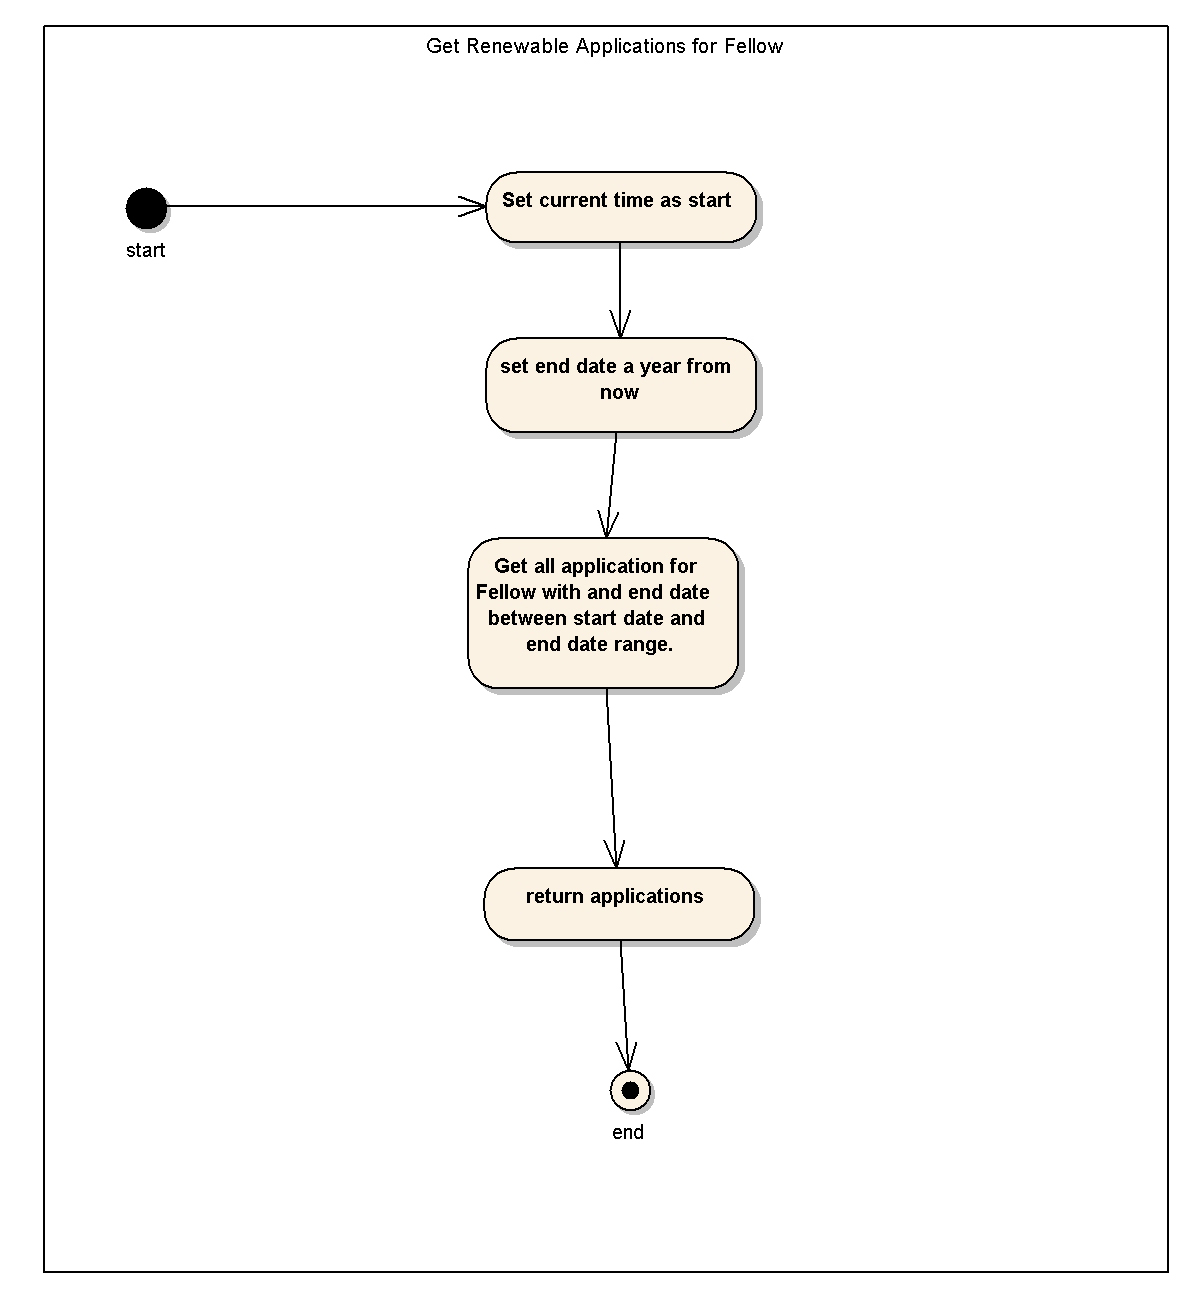
\includegraphics[scale=0.25]{../Images_Docs/Diagrams/Activity Diagrams/ApplicationRenewalService/Get Renewable Applications for Fellow.jpg}}
\caption{Activity diagram of the Get Renewable Applications for Fellow use case.}
\end{figure}

%%%%%%%%%%%%%%%%%%%%%%%%%%%%%%%%%%%%%%%%%%%%%%%%%%%%%%%%%%%%%%%%%%%%%%%%%%%%%%%%%%%%%%%%%%%%%%%%%%%%%%%%%%%%%%%%%%%%%%%%%%%%%%%%%%%%

\begin{figure}[H]
\centering	
\framebox{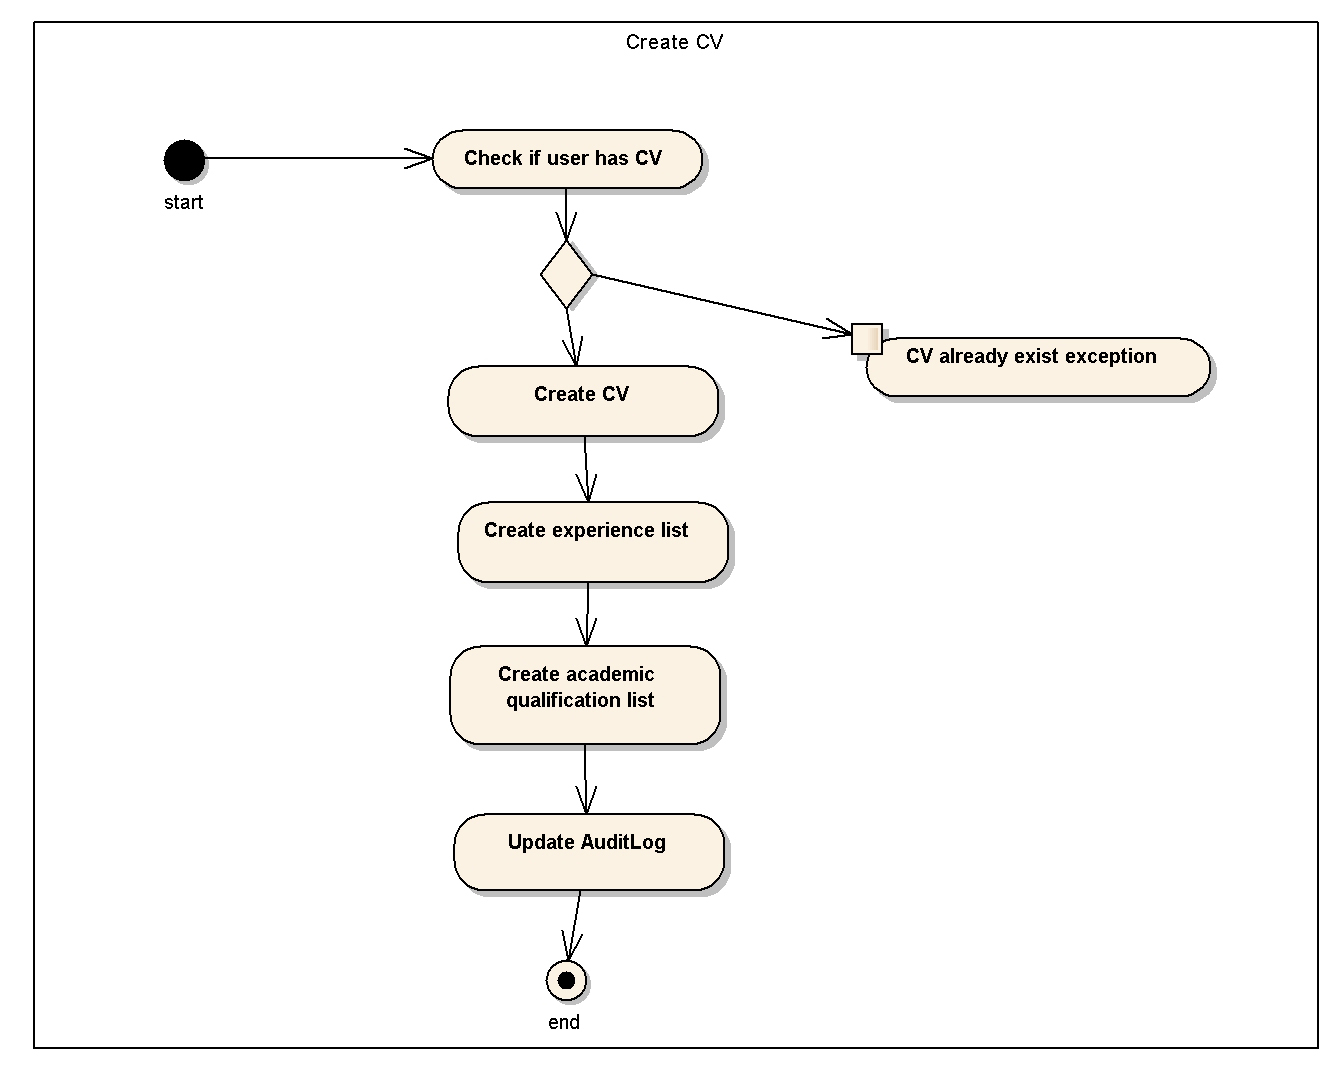
\includegraphics[scale=0.25]{../Images_Docs/Diagrams/Activity Diagrams/CV Management Service/Create CV.jpg}}
\caption{Activity diagram of the Create CV use case.}
\end{figure}

\begin{figure}[H]
\centering	
\framebox{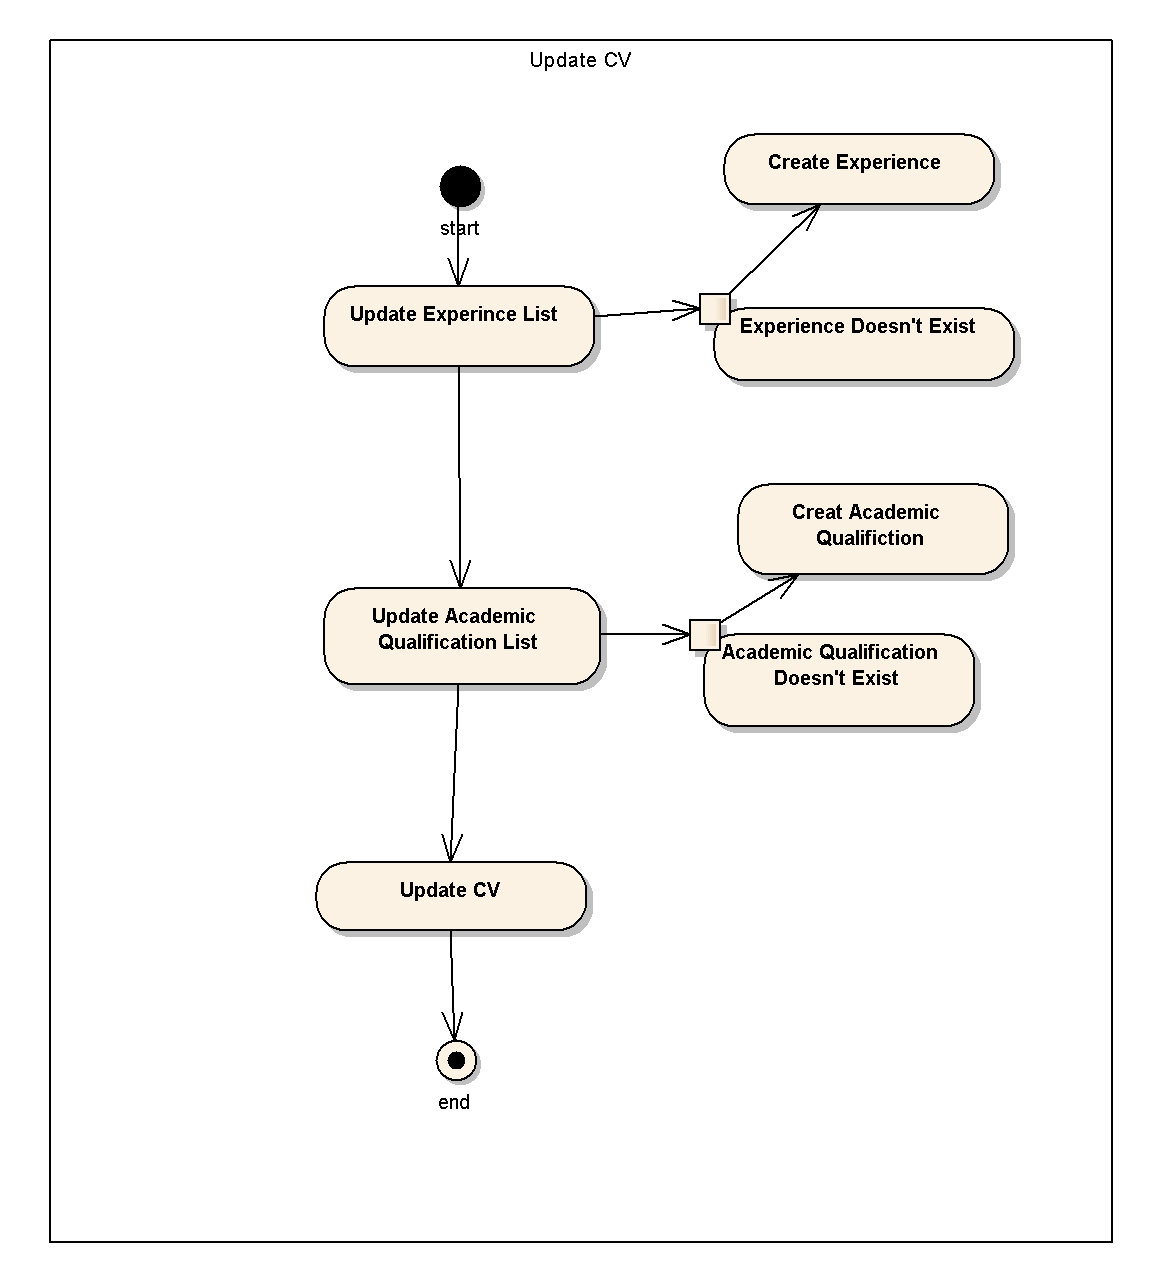
\includegraphics[scale=0.25]{../Images_Docs/Diagrams/Activity Diagrams/CV Management Service/Update CV.jpg}}
\caption{Activity diagram of the Update CV use case.}
\end{figure}

%%%%%%%%%%%%%%%%%%%%%%%%%%%%%%%%%%%%%%%%%%%%%%%%%%%%%%%%%%%%%%%%%%%%%%%%%%%%%%%%%%%%%%%%%%%%%%%%%%%%%%%%%%%%%%%%%%%%%%%%%%%%%%%%%%%%

\begin{figure}[H]
\centering	
\framebox{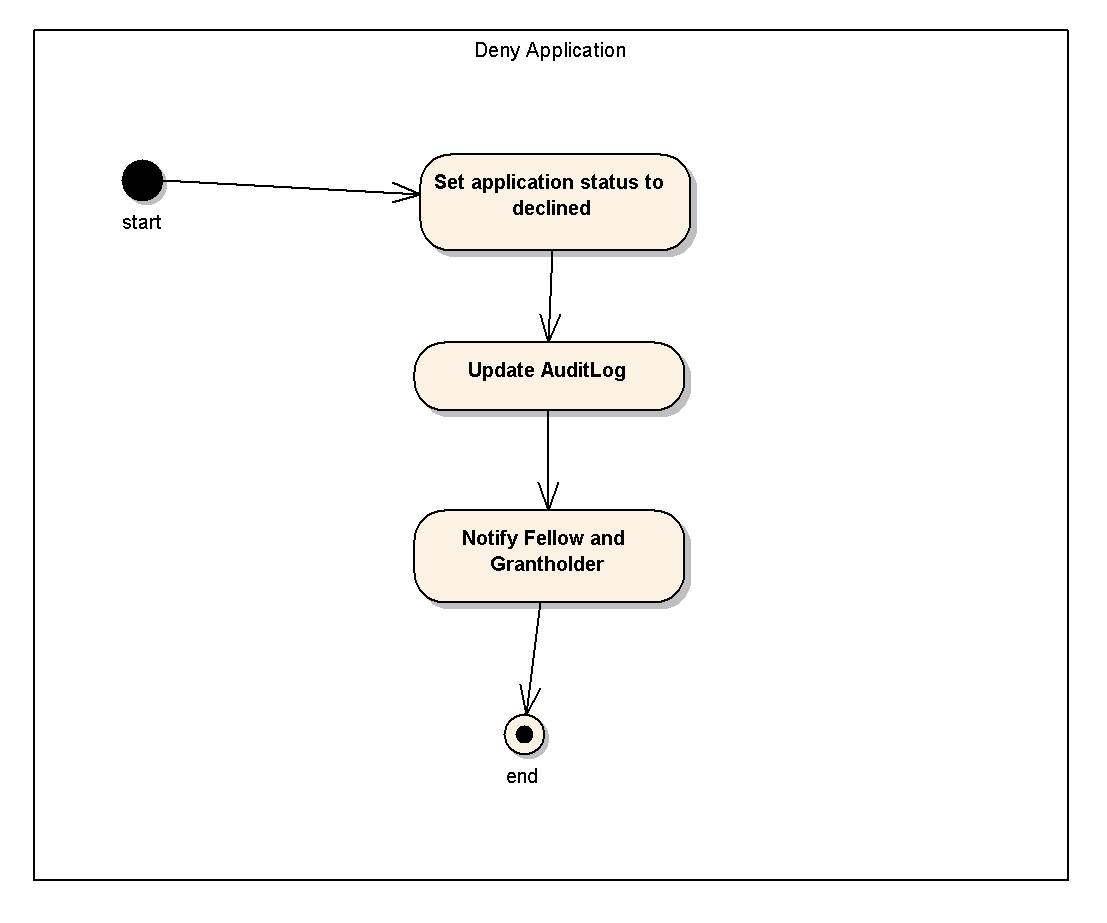
\includegraphics[scale=0.25]{../Images_Docs/Diagrams/Activity Diagrams/Dean Endorsement/Deny Application.jpg}}
\caption{Activity diagram of the Deny Application use case.}
\end{figure}

\begin{figure}[H]
\centering	
\framebox{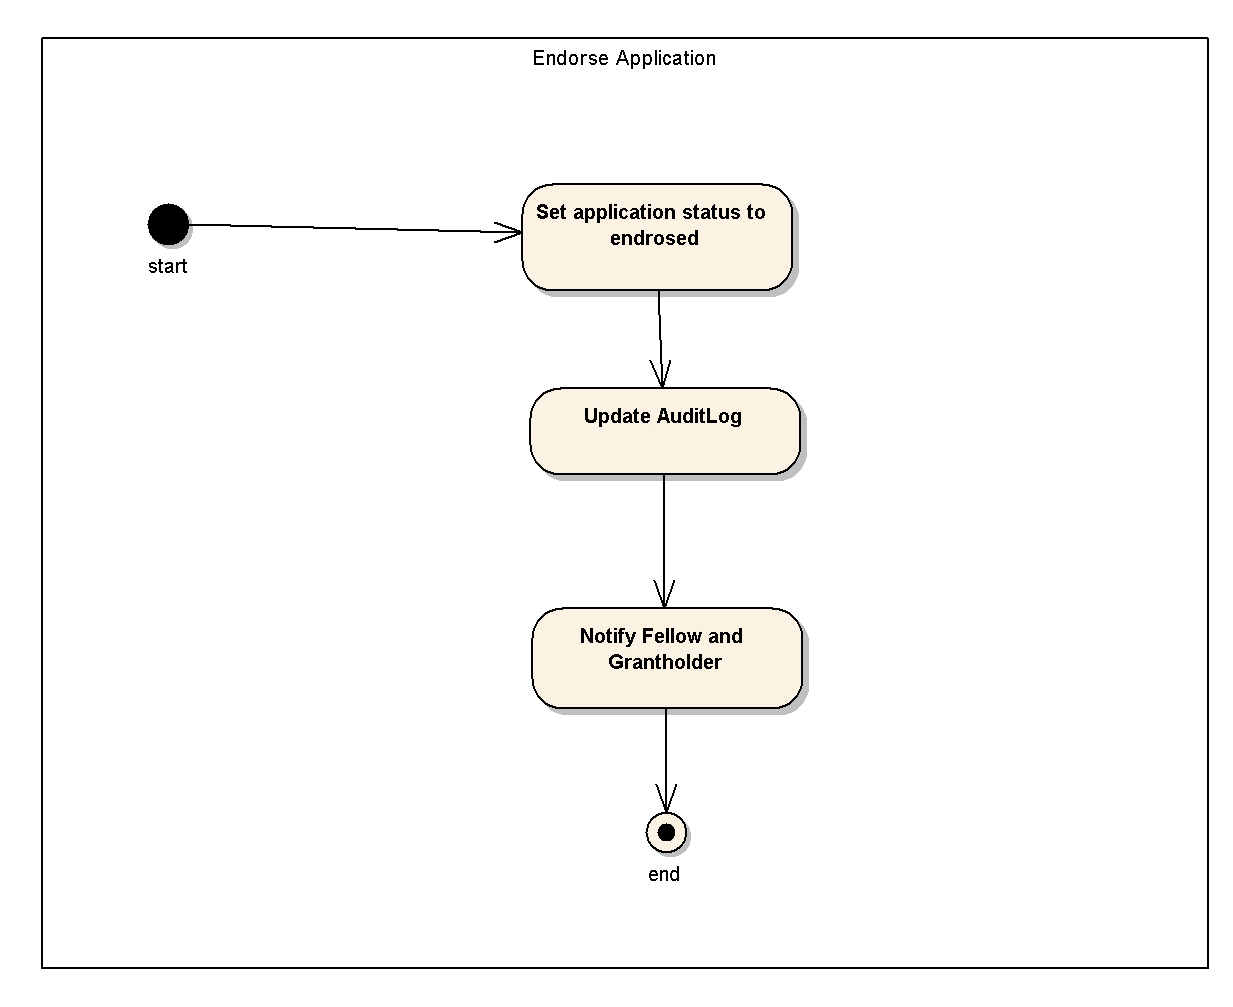
\includegraphics[scale=0.25]{../Images_Docs/Diagrams/Activity Diagrams/Dean Endorsement/Endorse Application.jpg}}
\caption{Activity diagram of the Endorse Application use case.}
\end{figure}

%%%%%%%%%%%%%%%%%%%%%%%%%%%%%%%%%%%%%%%%%%%%%%%%%%%%%%%%%%%%%%%%%%%%%%%%%%%%%%%%%%%%%%%%%%%%%%%%%%%%%%%%%%%%%%%%%%%%%%%%%%%%%%%%%%%%

\begin{figure}[H]
\centering	
\framebox{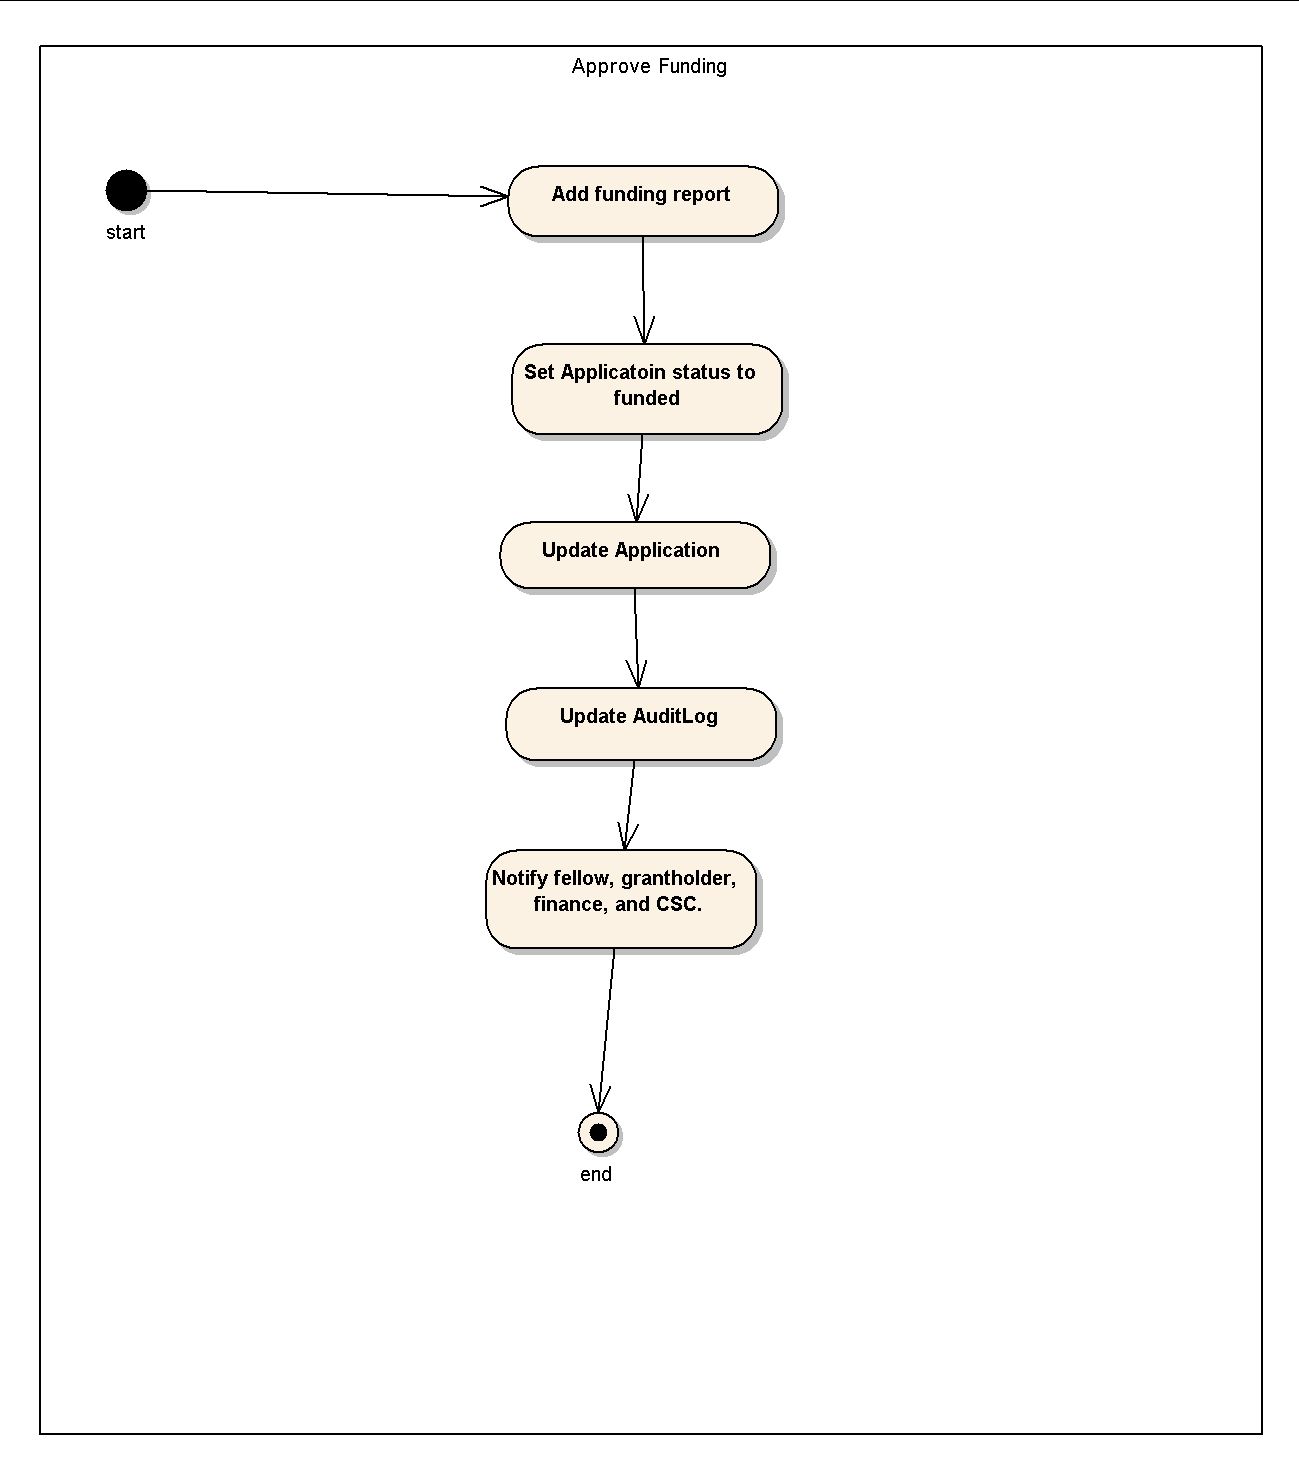
\includegraphics[scale=0.25]{../Images_Docs/Diagrams/Activity Diagrams/DRISApprovalService/Approve Funding.jpg}}
\caption{Activity diagram of the Approve Funding use case.}
\end{figure}

\begin{figure}[H]
\centering	
\framebox{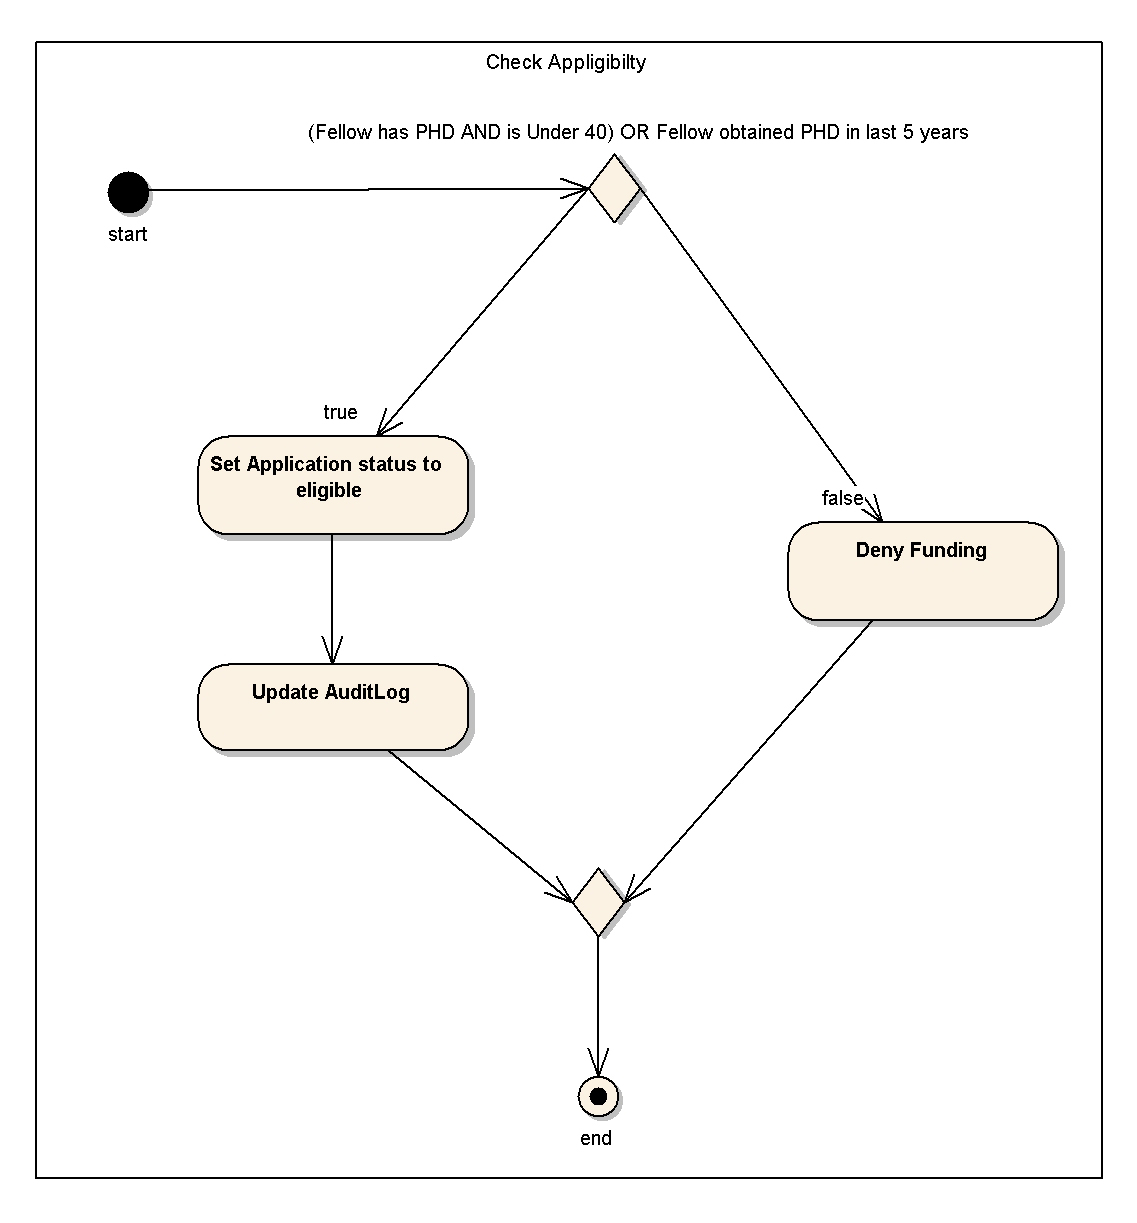
\includegraphics[scale=0.25]{../Images_Docs/Diagrams/Activity Diagrams/DRISApprovalService/Check Appligibilty.jpg}}
\caption{Activity diagram of the Check Appligibilty use case.}
\end{figure}

\begin{figure}[H]
\centering	
\framebox{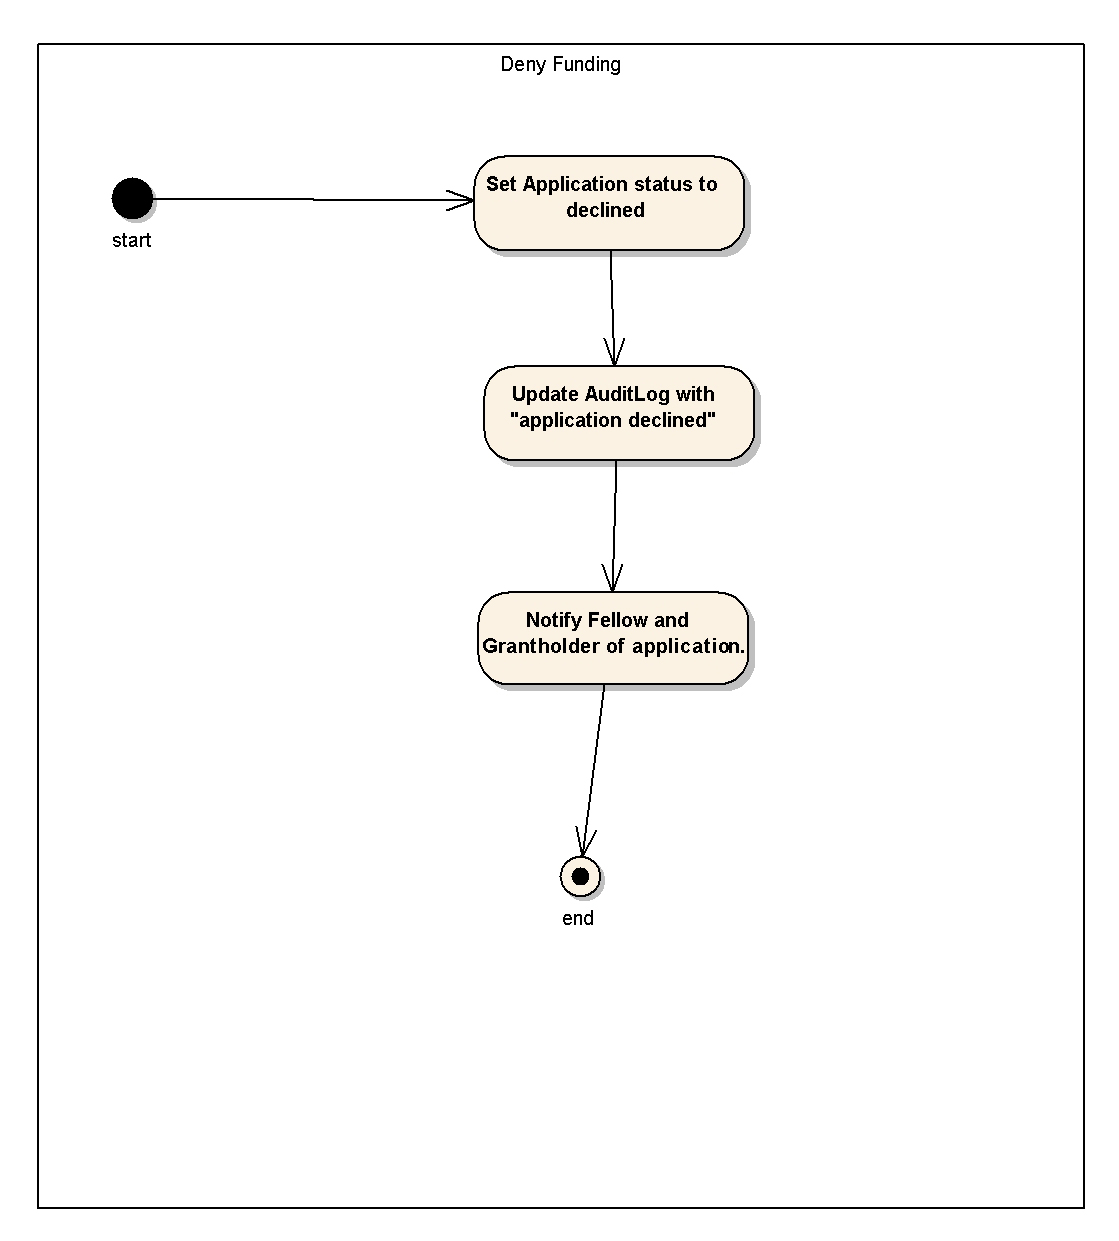
\includegraphics[scale=0.25]{../Images_Docs/Diagrams/Activity Diagrams/DRISApprovalService/Deny Funding.jpg}}
\caption{Activity diagram of the Deny Funding use case.}
\end{figure}

%%%%%%%%%%%%%%%%%%%%%%%%%%%%%%%%%%%%%%%%%%%%%%%%%%%%%%%%%%%%%%%%%%%%%%%%%%%%%%%%%%%%%%%%%%%%%%%%%%%%%%%%%%%%%%%%%%%%%%%%%%%%%%%%%%%%

\begin{figure}[H]
\centering	
\framebox{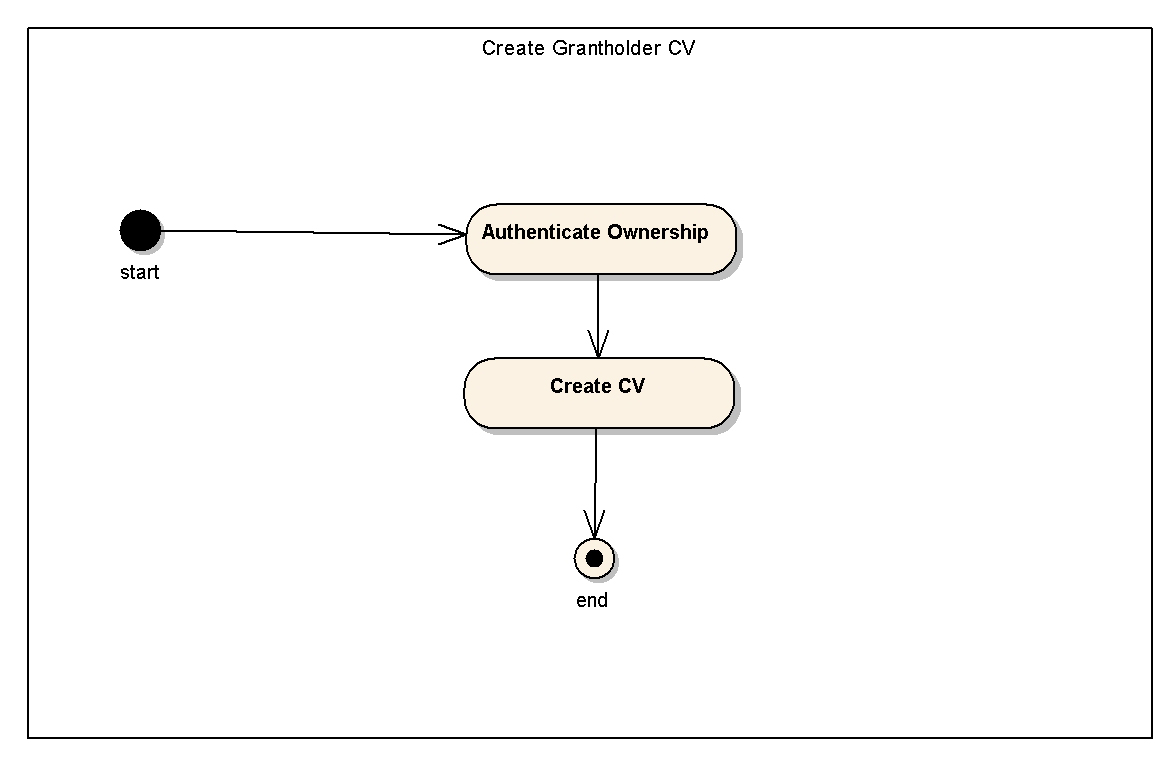
\includegraphics[scale=0.25]{../Images_Docs/Diagrams/Activity Diagrams/GrantHolderFinalisation/Create Grantholder CV.jpg}}
\caption{Activity diagram of the Create Grantholder CV use case.}
\end{figure}

\begin{figure}[H]
\centering	
\framebox{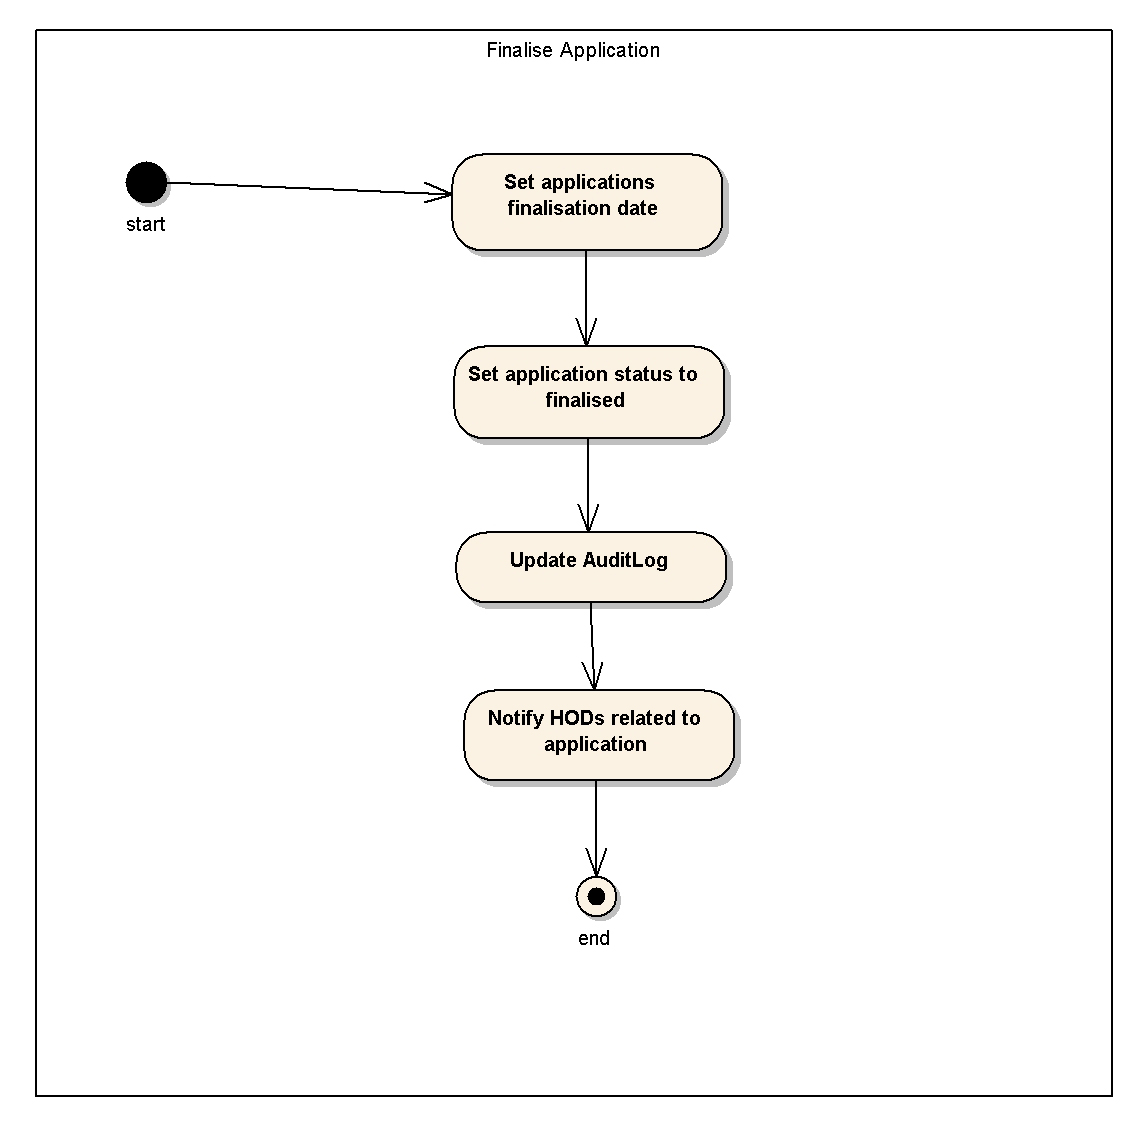
\includegraphics[scale=0.25]{../Images_Docs/Diagrams/Activity Diagrams/GrantHolderFinalisation/Finalise Application.jpg}}
\caption{Activity diagram of the Finalise Application use case.}
\end{figure}

%%%%%%%%%%%%%%%%%%%%%%%%%%%%%%%%%%%%%%%%%%%%%%%%%%%%%%%%%%%%%%%%%%%%%%%%%%%%%%%%%%%%%%%%%%%%%%%%%%%%%%%%%%%%%%%%%%%%%%%%%%%%%%%%%%%%

\begin{figure}[H]
\centering	
\framebox{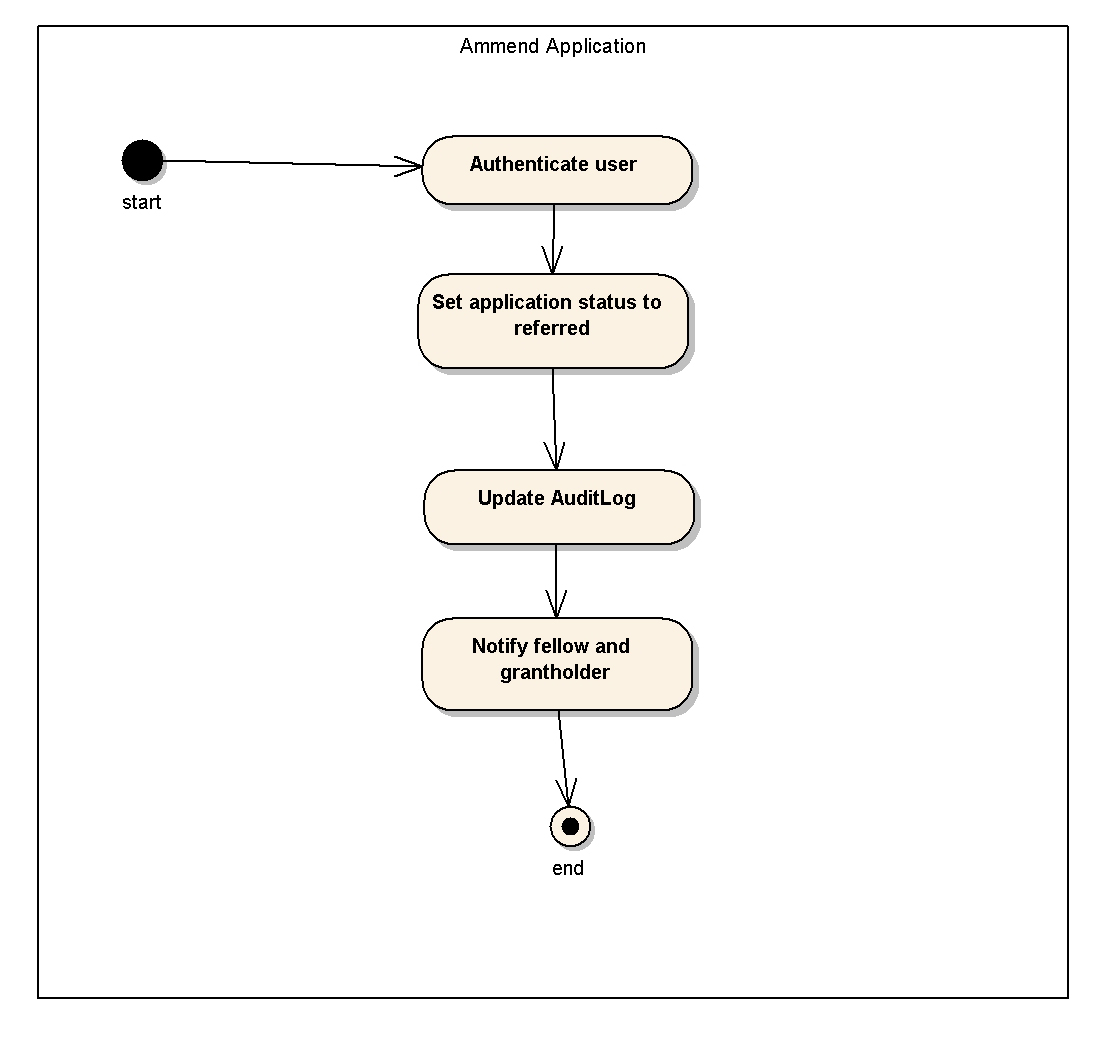
\includegraphics[scale=0.25]{../Images_Docs/Diagrams/Activity Diagrams/HOD recommendations/Ammend Application.jpg}}
\caption{Activity diagram of the Ammend Application use case.}
\end{figure}

\begin{figure}[H]
\centering	
\framebox{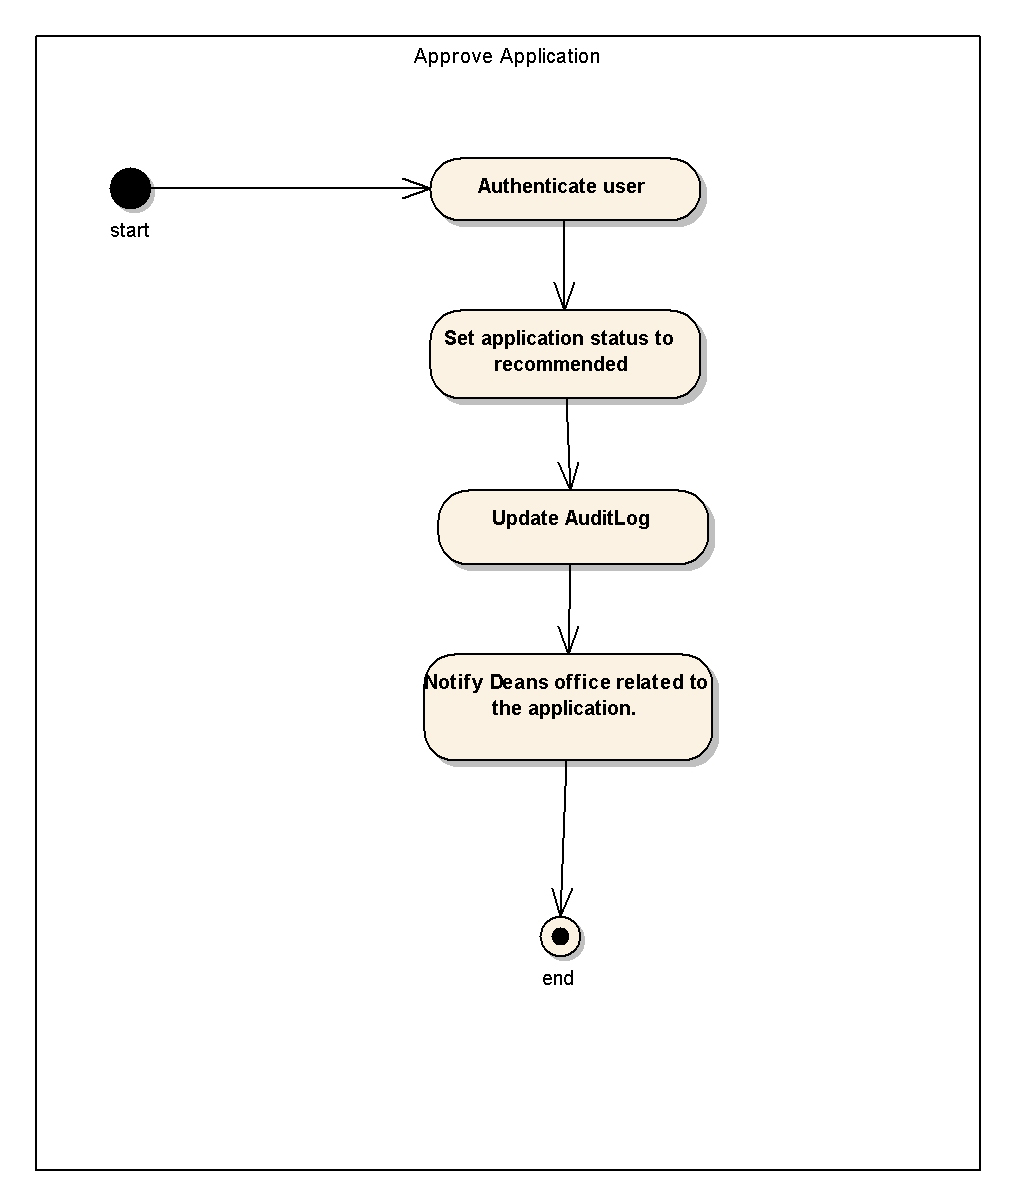
\includegraphics[scale=0.25]{../Images_Docs/Diagrams/Activity Diagrams/HOD recommendations/Approve Application.jpg}}
\caption{Activity diagram of the Approve Application use case.}
\end{figure}

\begin{figure}[H]
\centering	
\framebox{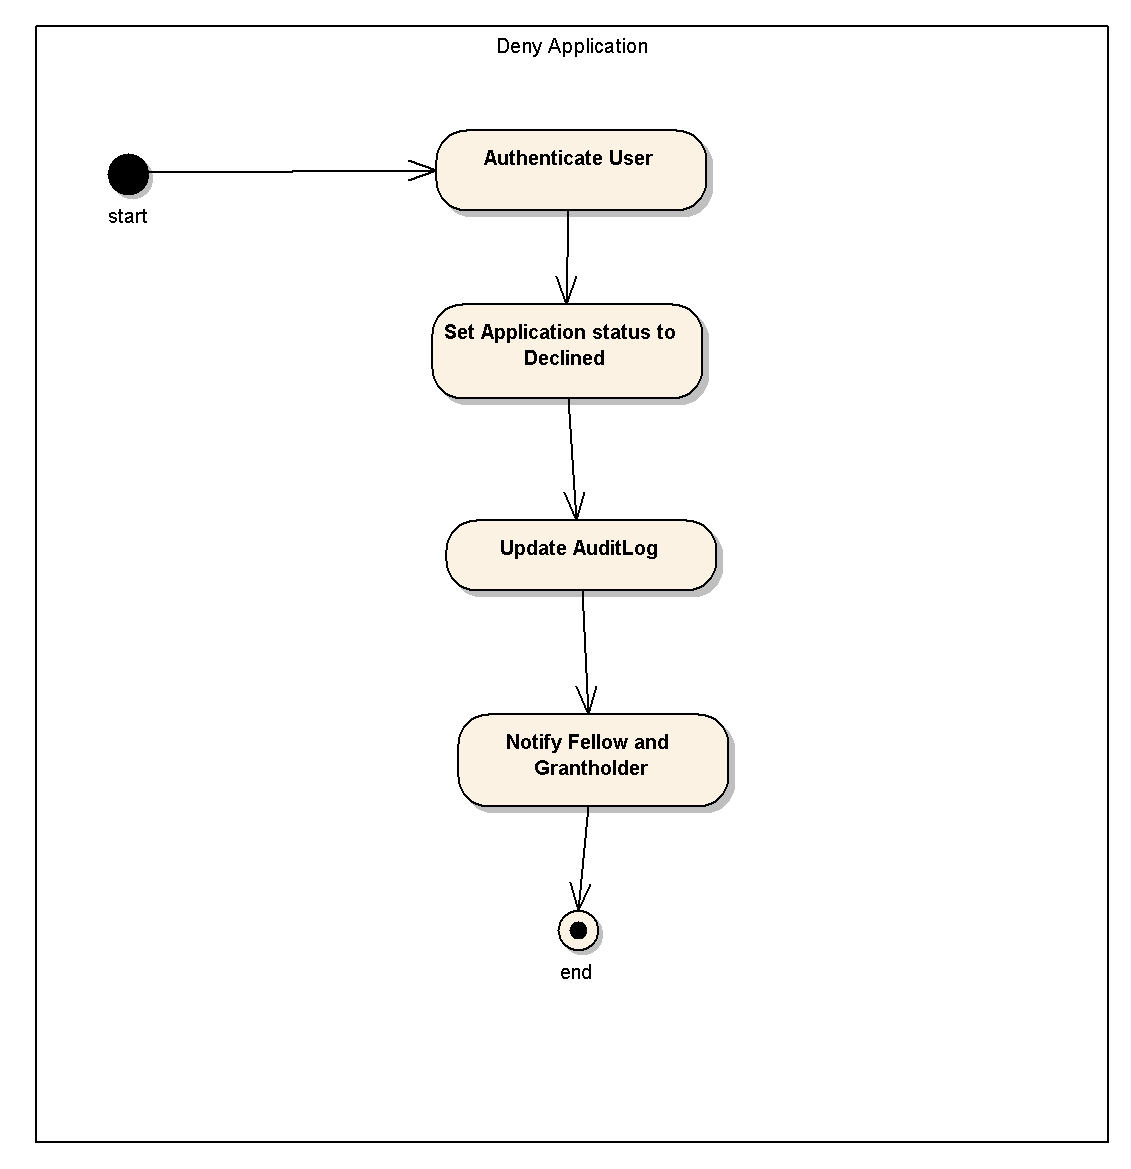
\includegraphics[scale=0.25]{../Images_Docs/Diagrams/Activity Diagrams/HOD recommendations/Deny Application.jpg}}
\caption{Activity diagram of the Deny Application use case.}
\end{figure}

\begin{figure}[H]
\centering	
\framebox{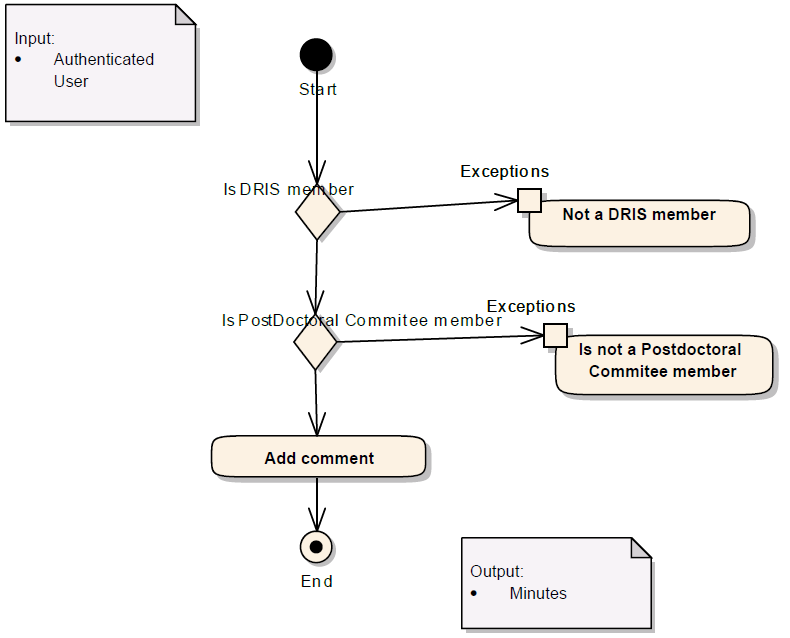
\includegraphics[scale=0.5]{../Images_Docs/Diagrams/Activity Diagrams/MeetingManagement/AddMinuteComment.png}}
\caption{Activity diagram of the Add Minute Comment use case.}
\end{figure}

\begin{figure}[H]
\centering	
\framebox{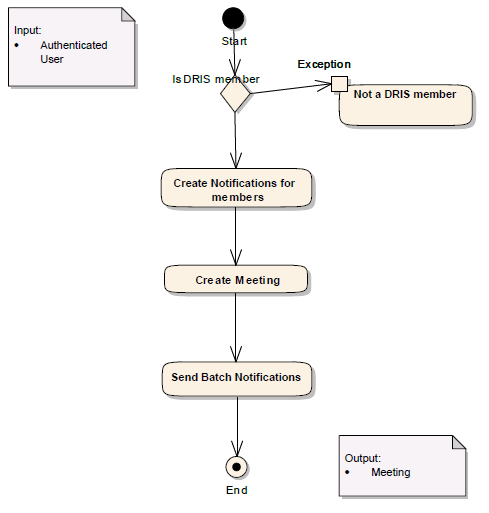
\includegraphics[scale=0.5]{../Images_Docs/Diagrams/Activity Diagrams/MeetingManagement/Meetings.png}}
\caption{Activity diagram of the Create Meeting use case.}
\end{figure}

\begin{figure}[H]
\centering	
\framebox{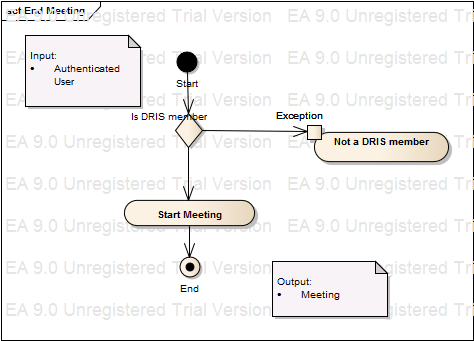
\includegraphics[scale=0.5]{../Images_Docs/Diagrams/Activity Diagrams/MeetingManagement/EndMeeting.png}}
\caption{Activity diagram of the End Meeting use case.}
\end{figure}

\begin{figure}[H]
\centering	
\framebox{\includegraphics[scale=0.5]{../Images_Docs/Diagrams/Activity Diagrams/MeetingManagement/GetAllActiveMeetings.png}}
\caption{Activity diagram of the Get All Active Meetings use case.}
\end{figure}

\begin{figure}[H]
\centering	
\framebox{\includegraphics[scale=0.5]{../Images_Docs/Diagrams/Activity Diagrams/MeetingManagement/GetAllMeetings.png}}
\caption{Activity diagram of the Get All Meetings use case.}
\end{figure}


\begin{figure}[H]
\centering	
\framebox{\includegraphics[scale=0.5]{../Images_Docs/Diagrams/Activity Diagrams/MeetingManagement/StartMeeting.png}}
\caption{Activity diagram of the Start Meeting use case.}
\end{figure}

\begin{figure}[H]
\centering		
\framebox{\includegraphics[scale=0.5]{../Images_Docs/Diagrams/Activity Diagrams/MeetingManagement/UpdateMeeting.png}}
\caption{Activity diagram of the Update Meeting use case.}
\end{figure}

\begin{figure}[H]
\centering	
\framebox{\includegraphics[scale=0.5]{../Images_Docs/Diagrams/Activity Diagrams/NewApplication/CanFellowOpenNewApplication.png}}
\caption{Activity diagram of the Can the fellow open a New Application use case.}
\end{figure}

\begin{figure}[H]
\centering	
\framebox{\includegraphics[scale=0.5]{../Images_Docs/Diagrams/Activity Diagrams/NewApplication/CreateCV.png}}
\caption{Activity diagram of the Create CV use case.}
\end{figure}

\begin{figure}[H]
\centering	
\framebox{\includegraphics[scale=0.5]{../Images_Docs/Diagrams/Activity Diagrams/NewApplication/NewApplication.png}}
\caption{Activity diagram of the Create New Application use case.}
\end{figure}

\begin{figure}[H]
\centering	
\framebox{\includegraphics[scale=0.5]{../Images_Docs/Diagrams/Activity Diagrams/NewApplication/CreateCV.png}}
\caption{Activity diagram of the Get Open Application use case.}
\end{figure}

\begin{figure}[H]
\centering	
\framebox{\includegraphics[scale=0.5]{../Images_Docs/Diagrams/Activity Diagrams/NewApplication/LinkGrantHolderToApplication.png}}
\caption{Activity diagram of the Link Grant Holder to Application use case.}
\end{figure}

\begin{figure}[H]
\centering	
\framebox{\includegraphics[scale=0.5]{../Images_Docs/Diagrams/Activity Diagrams/NewApplication/LinkRefereeToApplication.png}}
\caption{Activity diagram of the Link Referee to Application use case.}
\end{figure}

\begin{figure}[H]
\centering	
\framebox{\includegraphics[scale=0.5]{../Images_Docs/Diagrams/Activity Diagrams/NewApplication/SubmitApplication.png}}
\caption{Activity diagram of the Submit Application use case.}
\end{figure}

\begin{figure}[H]
\centering	
\framebox{\includegraphics[scale=0.5]{../Images_Docs/Diagrams/Activity Diagrams/Notifications/SendEmail.png}}
\caption{Activity diagram of the Get Notifications for Person use case.}
\end{figure}


\begin{figure}[H]
\centering	
\framebox{\includegraphics[scale=0.5]{../Images_Docs/Diagrams/Activity Diagrams/Notifications/GetNotificationsFromPerson.png}}
\caption{Activity diagram of the Get Notifications from Person use case.}
\end{figure}


\begin{figure}[H]
\centering	
\framebox{\includegraphics[scale=0.5]{../Images_Docs/Diagrams/Activity Diagrams/Notifications/SendBatchNotifications.png}}
\caption{Activity diagram of the Send batch Notifications use case.}
\end{figure}


\begin{figure}[H]
\centering	
\framebox{\includegraphics[scale=0.5]{../Images_Docs/Diagrams/Activity Diagrams/ProgressReportManagement/ProgressReport.png}}
\caption{Activity diagram of the Create Progress Report use case.}
\end{figure}

\begin{figure}[H]
\centering	
\framebox{\includegraphics[scale=0.5]{../Images_Docs/Diagrams/Activity Diagrams/ProgressReportManagement/UpdateProgressReport.png}}
\caption{Activity diagram of the Update Progress Report use case.}
\end{figure}

\begin{figure}[H]
\centering	
\framebox{\includegraphics[scale=0.5]{../Images_Docs/Diagrams/Activity Diagrams/RefereeReport/RefereesReport.png}}
\caption{Activity diagram of the Create Referee Report use case.}
\end{figure}

\begin{figure}[H]
\centering	
\framebox{\includegraphics[scale=0.5]{../Images_Docs/Diagrams/Activity Diagrams/RefereeReport/SubmitReferralReport.png}}
\caption{Activity diagram of the Submit Referee Report use case.}
\end{figure}

\begin{figure}[H]
\centering	
\framebox{\includegraphics[scale=0.5]{../Images_Docs/Diagrams/Activity Diagrams/RefereeReport/CountPendingApplications.png}}
\caption{Activity diagram of the Count Pending Reports use case.}
\end{figure}

\begin{figure}[H]
\centering	
\framebox{\includegraphics[scale=0.5]{../Images_Docs/Diagrams/Activity Diagrams/Reporting/ExportPDF.png}}
\caption{Activity diagram of the Export PDF Report use case.}
\end{figure}

\begin{figure}[H]
\centering	
\framebox{\includegraphics[scale=0.5]{../Images_Docs/Diagrams/Activity Diagrams/Reporting/ExportApplicationSpreadsheet.png}}
\caption{Activity diagram of the Export PDF Report use case.}
\end{figure}


\begin{figure}[H]
\centering	
\framebox{\includegraphics[scale=0.5]{../Images_Docs/Diagrams/Activity Diagrams/UserAccountManagement/GenerateSystemID.png}}
\caption{Activity diagram of the Generate System ID use case.}
\end{figure}

\begin{figure}[H]
\centering	
\framebox{\includegraphics[scale=0.5]{../Images_Docs/Diagrams/Activity Diagrams/UserAccountManagement/GetAllSecurityRoles.png}}
\caption{Activity diagram of the Get All Security Roles use case.}
\end{figure}

\begin{figure}[H]
\centering	
\framebox{\includegraphics[scale=0.5]{../Images_Docs/Diagrams/Activity Diagrams/UserAccountManagement/ViewAllAccounts.png}}
\caption{Activity diagram of the Get user by Email use case.}
\end{figure}

\begin{figure}[H]
\centering	
\framebox{\includegraphics[scale=0.5]{../Images_Docs/Diagrams/Activity Diagrams/UserAccountManagement/GetUserbySystemID.png}}
\caption{Activity diagram of the Get User by System ID use case.}
\end{figure}

\begin{figure}[H]
\centering	
\framebox{\includegraphics[scale=0.5]{../Images_Docs/Diagrams/Activity Diagrams/UserAccountManagement/RemoveUser.png}}
\caption{Activity diagram of the Remove User use case.}
\end{figure}

\begin{figure}[H]
\centering	
\framebox{\includegraphics[scale=0.5]{../Images_Docs/Diagrams/Activity Diagrams/UserAccountManagement/UpdateUserAccount.png}}
\caption{Activity diagram of the Update User use case.}
\end{figure}

\begin{figure}[H]
\centering	
\framebox{\includegraphics[scale=0.5]{../Images_Docs/Diagrams/Activity Diagrams/UserAccountManagement/ViewAllAccounts.png}}
\caption{Activity diagram of the View All Users use case.}
\end{figure}

\begin{figure}[H]
\centering	
\framebox{\includegraphics[scale=0.5]{../Images_Docs/Diagrams/Activity Diagrams/UserGateway/AuthenticateAsOwner.png}}
\caption{Activity diagram of the Authenticate User as Owner use case.}
\end{figure}

\begin{figure}[H]
\centering	
\framebox{\includegraphics[scale=0.5]{../Images_Docs/Diagrams/Activity Diagrams/UserGateway/GetUserFromSession.png}}
\caption{Activity diagram of the Get Http Session from Session use case.}
\end{figure}


\begin{figure}[H]
\centering	
\framebox{\includegraphics[scale=0.5]{../Images_Docs/Diagrams/Activity Diagrams/UserGateway/Logout.png}}
\caption{Activity diagram of the Logout use case.}
\end{figure}

\vspace{0.2in}
\newpage

\subsection{Interface Diagrams}
% Problem with having to many figures =========================================================================================

%\begin{figure}[H]
%\centering
%\subfloat[Interface Diagram for the Application Progress Viewer service][Application Progress Viewer service]{
%\framebox{\includegraphics[width=0.47\textwidth]{../Images_Docs/Diagrams/Interface Diagram/ApplicationProgressViewerService.jpg}}
%\label{fig:subfig1}}
%\subfloat[Interface Diagram for the Application Renewal service][Application Renewal service]{
%\framebox{\includegraphics[width=0.47\textwidth]{../Images_Docs/Diagrams/Interface Diagram/ApplicationRenewalService.jpg}}
%\label{fig:subfig2}}
%\qquad
%\subfloat[Interface Diagram for the Archival service][Archival service]{
%\framebox{\includegraphics[width=0.47\textwidth]{../Images_Docs/Diagrams/Interface Diagram/ArchivalService.jpg}}
%\label{fig:subfig3}}
%\subfloat[Interface Diagram for the CV Management service][CV Management service]{
%\framebox{\includegraphics[width=0.47\textwidth]{../Images_Docs/Diagrams/Interface Diagram/CVManagementService.jpg}}
%\label{fig:subfig4}}
%\qquad
%\subfloat[Interface Diagram for the Application Progress Viewer service][Application Progress Viewer service]{
%\framebox{\includegraphics[width=0.47\textwidth]{../Images_Docs/Diagrams/Interface Diagram/DeansEndorsementService.jpg}}
%\label{fig:subfig1}}
%\subfloat[Interface Diagram for the Application Renewal service][Application Renewal service]{
%\framebox{\includegraphics[width=0.47\textwidth]{../Images_Docs/Diagrams/Interface Diagram/DRISApprovalService.jpg}}
%\label{fig:subfig2}}
%\qquad
%\subfloat[Interface Diagram for the Archival service][Archival service]{
%\framebox{\includegraphics[width=0.47\textwidth]{../Images_Docs/Diagrams/Interface Diagram/GrantHolderFinalisationService.jpg}}
%\label{fig:subfig3}}
%\subfloat[Interface Diagram for the CV Management service][CV Management service]{
%\framebox{\includegraphics[width=0.47\textwidth]{../Images_Docs/Diagrams/Interface Diagram/HODRecommendationServices.jpg}}
%\label{fig:subfig4}}
%\caption{Interface diagrams}
%\label{fig:globfig}
%\end{figure}
% =================================================================================================================================

% Alternative implementation
\begin{figure}[H]

\begin{subfigure}[p]{0.47\textwidth}
\centering	
\framebox{\includegraphics[width=\textwidth]{../Images_Docs/Diagrams/Interface Diagram/ApplicationProgressViewerService.jpg}}
\caption{Interface Diagram for the Application Progress Viewer service.}
\end{subfigure}
~
\begin{subfigure}[p]{0.47\textwidth}
\centering	
\framebox{\includegraphics[width=\textwidth]{../Images_Docs/Diagrams/Interface Diagram/ApplicationRenewalService.jpg}}
\caption{Interface Diagram for the Application Renewal service.}
\end{subfigure}

\begin{subfigure}[p]{0.47\textwidth}
\centering	
\framebox{\includegraphics[width=\textwidth]{../Images_Docs/Diagrams/Interface Diagram/ArchivalService.jpg}}
\caption{Interface Diagram for the Archival service.}
\end{subfigure}
~
\begin{subfigure}[p]{0.47\textwidth}
\centering	
\framebox{\includegraphics[width=\textwidth]{../Images_Docs/Diagrams/Interface Diagram/CVManagementService.jpg}}
\caption{Interface Diagram for the CV Management service.}
\end{subfigure}

\begin{subfigure}[p]{0.47\textwidth}
\centering	
\framebox{\includegraphics[width=\textwidth]{../Images_Docs/Diagrams/Interface Diagram/DeansEndorsementService.jpg}}
\caption{Interface Diagram for the Deans Endorsement service.}
\end{subfigure}
~
\begin{subfigure}[p]{0.47\textwidth}
\centering	
\framebox{\includegraphics[width=\textwidth]{../Images_Docs/Diagrams/Interface Diagram/DRISApprovalService.jpg}}
\caption{Interface Diagram for the DRIS Approval service.}
\end{subfigure}
\end{figure}

\begin{figure}[H]
\begin{subfigure}[p]{0.47\textwidth}
\centering	
\framebox{\includegraphics[width=\textwidth]{../Images_Docs/Diagrams/Interface Diagram/GrantHolderFinalisationService.jpg}}
\caption{Interface Diagram for the Grant Holder Finalisation service.}
\end{subfigure}
~
\begin{subfigure}[p]{0.47\textwidth}
\centering	
\framebox{\includegraphics[width=\textwidth]{../Images_Docs/Diagrams/Interface Diagram/HODRecommendationServices.jpg}}
\caption{Interface Diagram for the HOD Recommendation service.}
\end{subfigure}

\begin{subfigure}[H]{0.47\textwidth}
\centering	
\framebox{\includegraphics[width=\textwidth]{../Images_Docs/Diagrams/Interface Diagram/MeetingMananagementInterface.png}}
\caption{Interface Diagram for the Meeting Management service.}
\end{subfigure}
~
\begin{subfigure}[H]{0.47\textwidth}
\centering	
\framebox{\includegraphics[scale=0.5]{../Images_Docs/Diagrams/Interface Diagram/NewApplicationServiceInterface.png}}
\caption{Interface Diagram for the New Application service.}
\end{subfigure}

\begin{subfigure}[H]{0.47\textwidth}
\centering	
\framebox{\includegraphics[width=\textwidth]{../Images_Docs/Diagrams/Interface Diagram/NotificationsInterface.png}}
\caption{Interface Diagram for the Notification service.}
\end{subfigure}
~
\begin{subfigure}[H]{0.47\textwidth}
\centering	
\framebox{\includegraphics[width=\textwidth]{../Images_Docs/Diagrams/Interface Diagram/ProgressReportManagementServiceInterface.png}}
\caption{Interface Diagram for the Progress Report Management service.}
\end{subfigure}
\end{figure}

\begin{figure}[H]
\begin{subfigure}[H]{0.47\textwidth}
\centering	
\framebox{\includegraphics[width=\textwidth]{../Images_Docs/Diagrams/Interface Diagram/RefereeReportInterface.png}}
\caption{Interface Diagram for the Referee Report service.}
\end{subfigure}
~
\begin{subfigure}[H]{0.47\textwidth}
\centering	
\framebox{\includegraphics[width=\textwidth]{../Images_Docs/Diagrams/Interface Diagram/UserAccountManagementServicesInterface.png}}
\caption{Interface Diagram for the User Account Management service.}
\end{subfigure}

\begin{subfigure}[H]{0.47\textwidth}
\centering	
\framebox{\includegraphics[width=\textwidth]{../Images_Docs/Diagrams/Interface Diagram/UserGatewayInterface.png}}
\caption{Interface Diagram for the User Gateway service.}
\end{subfigure}

%%%%%%%%%%%%%%%%%%%%%%%%%%%%%%%%%%%%%%%%%%%%%%%%%%%%%%%%%%%%%%%%%%%%%%%%%%%%%%%%%%%%%%%%%%%%%%%%%%%%%
\end{figure}
\newpage
\subsection{Data Flow Diagrams}
\begin{figure}


\begin{subfigure}[p]{0.47\textwidth}
\centering	
\framebox{\includegraphics[width=\textwidth]{../Images_Docs/Diagrams/Data Flow/ApplicationProgress.png}}
\caption{Data Flow for Application progress viewer.}
\end{subfigure}

\begin{subfigure}[p]{0.47\textwidth}
\centering	
\framebox{\includegraphics[width=\textwidth]{../Images_Docs/Diagrams/Data Flow/ApplicationRenewal.png}}
\caption{Data Flow for Application Renewal.}
\end{subfigure}

\begin{subfigure}[p]{0.47\textwidth}
\centering	
\framebox{\includegraphics[width=\textwidth]{../Images_Docs/Diagrams/Data Flow/ArchivalService.png}}
\caption{Data Flow for Archival Service.}
\end{subfigure}

\begin{subfigure}[p]{0.47\textwidth}
\centering	
\framebox{\includegraphics[width=\textwidth]{../Images_Docs/Diagrams/Data Flow/AuditTrail.png}}
\caption{Data Flow for Audit Trail.}
\end{subfigure}

\begin{subfigure}[p]{0.47\textwidth}
\centering	
\framebox{\includegraphics[width=\textwidth]{../Images_Docs/Diagrams/Data Flow/CVManagement.png}}
\caption{Data Flow CV Management.}
\end{subfigure}

\begin{subfigure}[p]{0.47\textwidth}
\centering	
\framebox{\includegraphics[width=\textwidth]{../Images_Docs/Diagrams/Data Flow/DeansEndorsement.png}}
\caption{Data Flow for Dean's Endorsement.}
\end{subfigure}

\begin{subfigure}[p]{0.47\textwidth}
\centering	
\framebox{\includegraphics[width=\textwidth]{../Images_Docs/Diagrams/Data Flow/DRISApproval.png}}
\caption{Data Flow for DRIS Approval.}
\end{subfigure}

\begin{subfigure}[p]{0.47\textwidth}
\centering	
\framebox{\includegraphics[width=\textwidth]{../Images_Docs/Diagrams/Data Flow/GrantHolderFinalisation.png}}
\caption{Data Flow for Grant Holder Finalisation.}
\end{subfigure}

\begin{subfigure}[p]{0.47\textwidth}
\centering	
\framebox{\includegraphics[width=\textwidth]{../Images_Docs/Diagrams/Data Flow/HODRecommendation.png}}
\caption{Data Flow for HOD Recommendation.}
\end{subfigure}

\begin{subfigure}[p]{0.47\textwidth}
\centering	
\framebox{\includegraphics[width=\textwidth]{../Images_Docs/Diagrams/Data Flow/MeetingManagement.png}}
\caption{Data Flow for Meeting Management.}
\end{subfigure}

\begin{subfigure}[p]{0.47\textwidth}
\centering	
\framebox{\includegraphics[width=\textwidth]{../Images_Docs/Diagrams/Data Flow/NewApplication.png}}
\caption{Data Flow for New Application .}
\end{subfigure}

\begin{subfigure}[p]{0.47\textwidth}
\centering	
\framebox{\includegraphics[width=\textwidth]{../Images_Docs/Diagrams/Data Flow/NotificationService.png}}
\caption{Data Flow for Notification Service.}
\end{subfigure}

\begin{subfigure}[p]{0.47\textwidth}
\centering	
\framebox{\includegraphics[width=\textwidth]{../Images_Docs/Diagrams/Data Flow/ProgressReport.png}}
\caption{Data Flow for Progress Reports.}
\end{subfigure}

\begin{subfigure}[p]{0.47\textwidth}
\centering	
\framebox{\includegraphics[width=\textwidth]{../Images_Docs/Diagrams/Data Flow/RefereeReport.png}}
\caption{Data Flow for Referee Report.}
\end{subfigure}

\begin{subfigure}[p]{0.47\textwidth}
\centering	
\framebox{\includegraphics[width=\textwidth]{../Images_Docs/Diagrams/Data Flow/Reporting.png}}
\caption{Data Flow for Reporting Service.}
\end{subfigure}

\begin{subfigure}[p]{0.47\textwidth}
\centering	
\framebox{\includegraphics[width=\textwidth]{../Images_Docs/Diagrams/Data Flow/UserAccount.png}}
\caption{Data Flow for User Account Management.}
\end{subfigure}

\begin{subfigure}[p]{0.47\textwidth}
\centering	
\framebox{\includegraphics[width=\textwidth]{../Images_Docs/Diagrams/Data Flow/UserGateway.png}}
\caption{Data Flow for User Gateway.}
\end{subfigure}


\end{figure}
\vspace{0.2in}
\newpage
\subsection{Domain Objects}
\subsubsection{Overview}

\begin{figure}[H]
\centering	
\framebox{\includegraphics[scale=0.45]{../Images_Docs/Diagrams/DomainObjects/DomainObjects1.png}}
\caption{Overview of the data structures and relationships for the core domain objects of the
system.}
\end{figure}

\newpage
\subsubsection{Person}
This object represents the stakeholders that will make use of the system. All stakeholders will have accounts which they will use to log on to the system, using a unique user id and a predefined or user specified password. The unique user id can either be a Peoplesoft Emplid number or a email address. The person has an associated \textbf{Location} and \textbf{SecurityRole}(s)

\subsubsection{Department}
This object represents the department under which a \textbf{Person} falls in the \textbf{Faculty}. This is used to if they are a \textbf{employee} or \textbf{Research fellow} at the University of Pretoria. This object will no longer be needed if the system is integrated with peoplesoft as it would cause redundancy.

\subsubsection{Faculty}
This object represents the faculty that may exist under an institution. It is used to map the location of a \textbf{Person}. 

\subsubsection{Institution}
This object represents the institutions that may exist in the system. It is used to map the location of a \textbf{Person}. This allows for generic support if the software solution had to be expanded to other universities.

\subsubsection{EmployeeInformation}
This object represents the information regarding the employment of a \textbf{Person} at the University. It also contains the \textbf{Department} under which the \textbf{Person} falls. Also it contains the physical \textbf{Address} of the employee's office. This is made generic for software expansion support.  

\subsubsection{ResearchFellowInformation}
This object represents the CSC's or institution equivalents assigned emplid and the institution's assigned email address for an appointed \textbf{ResearchFellow}. This allows for possible future integration and better user support. Also it stores the \textbf{Department} in the institution to which the fellow was assigned to by the \textbf{DRIS}.

\subsubsection{Address}
This object represents a physical address. Thus it is used to expand and provide location details for a particular physical object or person.  

\subsubsection{SecurityRole}
This object represents a particular security role of a \textbf{Person}. A \textbf{Person} may have many different security roles. The security role can be used as a subtype discriminator for relational database architectures.

\subsubsection{DRIS}
This object represents members of Department of Research and Innovation Support who administers the process.

\subsubsection{FundingReport}
This object represents an \textbf{Application}'s funding costs as decide per the \textbf{DRIS}. It comprises of multiple \textbf{FundingCost}s that provides the various funding inputs from various parties for the particular fund-able costs namely fellowship, travel, running, equipment, operating
and conference.
 
\subsubsection{FundingCost}
This object represents a particular funding input cost for a \textbf{Application} from a particular funder. 

\subsubsection{DeclineReport}
This object represents the report associated with an \textbf{Application} that has been declined by some authority. It contains the creation timestamp, \textbf{Person} responsible and the reason. Only one such report can exist per \textbf{Application}.

\subsubsection{AmmendRequest}
This object represents a Amend request for a \textbf{Application} that is sent by some \textbf{HOD}. It contains the creation timestamp, \textbf{HOD} responsible and the reason. This is used to allow fellow to understand what is wrong with their \textbf{Application} so that they can correct it. There can be multiple such requests associated with an \textbf{Application}.

\subsubsection{EligibilityReport}
This object represents a report associated with an \textbf{Application} that has been checked for eligibility. It contains the check timestamp and \textbf{DRIS} member responsible. It is primary used for auditing. Only one such report can exist per \textbf{Application}.

\subsubsection{ForwardAndRewindReport}
This object represents a report associated with an \textbf{Application} that has been either forwarded or re-winded through a particular set of application stages. This is used to track such actions and the reasons for them. There can be multiple such reports associated with an \textbf{Application}. 
 
\subsubsection{ProspectiveFellow}
This inherited object represents a prospective fellow who is a holder of a PhD obtained in the last five years (or nearing completion of a PhD) or is 40 years or younger and has a PhD. The prospective fellow can open a \textbf{NewApplication}.

\subsubsection{ResearchFellow}
This inherited object represents a research fellow who is a currently a researcher at the University of Pretoria. This object was initially a \textbf{ProspectiveFellow}. The research fellow can apply for a \textbf{RenewalApplication} if their application falls in their renewal time frame.

\subsubsection{GrantHolder}
This inherited object represents a grant holder who can be a rated researcher by the NRF or not. The system should not require the CV's of A and B rated researchers to be added to the system. The reason for this is that the CV's of such researchers can be easily obtained from the NRF and tend to be very long. A grant holder is the supervisor for a or many \textbf{ProspectiveFellow}(s) or \textbf{ResearchFellow}(s) and owns the \textbf{Application} of the \textbf{ProspectiveFellow}(s) or \textbf{ResearchFellow}(s).

\subsubsection{HOD}
This inherited object represents a HOD of a particular department. The HOD creates the recommendation reports for \textbf{Application}(s) they consider to meet their requirements.\\

\subsubsection{HODRecommandationReport}
This inherited object represents a recommendation report highlighting the reasons to why the \textbf{Application} of a \textbf{ProspectiveFellow} or \textbf{ResearchFellow} is needed by the department.

\subsubsection{Deans Office}
The Dean's office object represents the relevant faculty's Dean and Deputy Dean. The Dean's Office creates the \textbf{Endorsement} for any the \textbf{Application} that is approved by them.

\subsubsection{Endorsement}
This object represents the endorsement of an \textbf{Application} of a \textbf{ProspectiveFellow} or \textbf{ResearchFellow} and contains the rank in comparison to other pending \textbf{Application}(s) with a \textbf{Endorsement}.

\subsubsection{Referee}
This inherited object represents the referees of any \textbf{ProspectiveFellow} and is responsible for creating \textbf{RefereeReport} regarding the \textbf{ProspectiveFellow}.

\subsubsection{RefereeReport}
This object represents the referral report from an identified referee of a \textbf{ProspectiveFellow}.

\subsubsection{PostDocCommittee}
This inherited object represents the individual members of the post-doctoral committee who approves all available \textbf{Applications} during committee meetings and records the \textbf{Minutes} of the meeting.

\subsubsection{CommitteeMeeting}
This object represents a meeting of the \textbf{PostDocCommittee} convened by the \textbf{DRIS} that will be review the \textbf{Applications} and will evaluate each. This object contains the attendance list, date and time convened and the \textbf{MinuteComment}s of the meeting.

\subsubsection{MinuteComment}
This object represents a comment made by a \textbf{PostDocCommittee} member during a \textbf{CommitteeMeeting}.

\subsubsection{Application}
This object represents an applications and will contain the information of \textbf{ProspectiveFellow} or \textbf{ResearchFellow} and \textbf{GrantHolder} who owns it. The object holds the status of the application and any project information. As well as the \textbf{HODRecommandationReport} of a \textbf{HOD} and \textbf{Endorsement} from a \textbf{DeansOffice}. It further holds the \textbf{EligibilityReport} and \textbf{FundingReport} from the \textbf{DRIS}. If the application is declined the \textbf{DeclineReport} is associated with the application. The application object can also hold multiple \textbf{AmmendRequest}s if any such requests are created. All the \textbf{ProgressReport}s created by the \textbf{ResearchFellow} are also contained in the application. Lastly if the application forwarded or re-winded then the associated \textbf{Forward rewind report}s are also contained by the application 

\subsubsection{NewApplication}
This inherited object represents new application for a \textbf{ProspectiveFellow} who is currently not a fellow in the system. Also it holds any \textbf{RefereeReport}(s) that has been created for the application.

\subsubsection{RenewalApplication}
This inherited object represents renewal application for a \textbf{ProspectiveFellow} who is a fellow in the system. Also it holds the \textbf{ProgressReport} that has been created for the application.

\subsubsection{ProgressReport}
This object represents the periodical report on the research that the \textbf{ResearchFellow} has done for the particular period in the duration of their fellowship. These reports are completed on an annual bases.

\subsubsection{CV}
This object represents a CV and contains all the information such as personal details, \textbf{AcademicQualification}(s), \textbf{Experience} regarding a \textbf{GrantHolder} or \textbf{ProspectiveFellow} in the system.

\subsubsection{AcademicQualification}
This object represents a academic qualification and the information regarding it such as the qualification name, field, where it was obtained and when it was obtained.

\subsubsection{Experience}
This object represents a work experience and the information regarding it such as the capacity of the work, where this work was done and when it was done.

\subsubsection{Notification}
This object represents a email or internal message sent by a user to a user via the system. The system itself may also seen as a user with regards to the sender of such notification. It consists of the actual message, subject, timestamp and email status. 

\subsubsection{AuditLog}
This object represents a audit log that stores all the actions of all users within the system. Each entry records the action, who committed the action as well as at what time the action was committed.

\subsubsection{Session}
This object represents a the details of a currently active session on the system. It contains the user (\textbf{Person}) and the link to the system's session management system's record. This object will be used through out the system for auditing and authentication. 

\newpage

\section{Glossary:}
\vspace{0.2in}

\begin{itemize}
\item \textbf{Activity diagram} - A UML diagram that depicts the flow of actions or activities in the process.
\item \textbf{API} - Application Programming Interface
\item \textbf{Audit log} - A log that keeps track of user actions.
\item \textbf{Application} -Both renewal applications or new fellowship applications are seen as applications by this project.
\item \textbf{CV} - Curriculum Vita
\item \textbf{Domain objects} - Are the objects that are present in the system being modelled.
\item \textbf{HTML} - Hyper Text Mark-up Language
\item \textbf{Java EE} - Java Enterprise Edition
\item \textbf{NRF} - National Research Foundation
\item \textbf{PhD} - A doctoral degree in a particular field of study.
\item \textbf{PDF} - Portable Document Format file
\item \textbf{Peoplesoft} - A management system designed by oracle. 
\item \textbf{Spreadsheet} - A special type of digital document that is used to represent data in rows and columns
\item \textbf{Use case diagram} - A UML diagram that gives a visual depiction of a service or group of services.
\item \textbf{UML} - Unified modelling language. A commonly used model standard to provide technology neutral models of different aspects of software.
\item \textbf{UP} - University of Pretoria
 


\end{itemize}	

\end{document}